%%%%%%%%%%%%%%%%%%%%%%%%%%%%%%%%%%%%%%%%%%%%%%%%%%%%%%%%%%%%%%%%%%%%%%%%%%%%
% AGUtmpl.tex: this template file is for articles formatted with LaTeX2e,
% Modified July 2011
%
% This template includes commands and instructions
% given in the order necessary to produce a final output that will
% satisfy AGU requirements.
%
% PLEASE DO NOT USE YOUR OWN MACROS
% DO NOT USE \newcommand, \defcommand, or \renewcommand.
%
% FOR FIGURES, DO NOT USE \psfrag or \subfigure.
%
%%%%%%%%%%%%%%%%%%%%%%%%%%%%%%%%%%%%%%%%%%%%%%%%%%%%%%%%%%%%%%%%%%%%%%%%%%%%
%
% All questions should be e-mailed to latex@agu.org.
%
%%%%%%%%%%%%%%%%%%%%%%%%%%%%%%%%%%%%%%%%%%%%%%%%%%%%%%%%%%%%%%%%%%%%%%%%%%%%
%
% Step 1: Set the \documentclass
%
% There are two options for article format: two column (default)
% and draft.
%
% PLEASE USE THE DRAFT OPTION TO SUBMIT YOUR PAPERS.
% The draft option produces double spaced output.
%
% Choose the journal abbreviation for the journal you are
% submitting to:

% jgrga JOURNAL OF GEOPHYSICAL RESEARCH
% gbc   GLOBAL BIOCHEMICAL CYCLES
% grl   GEOPHYSICAL RESEARCH LETTERS
% pal   PALEOCEANOGRAPHY
% ras   RADIO SCIENCE
% rog   REVIEWS OF GEOPHYSICS
% tec   TECTONICS
% wrr   WATER RESOURCES RESEARCH
% gc    GEOCHEMISTRY, GEOPHYSICS, GEOSYSTEMS
% sw    SPACE WEATHER

% (If you are submitting to a journal other than jgrga,
% substitute the initials of the journal for "jgrga" below.)

\documentclass[draft,jgrga]{AGUTeX}

%%%%%%%%%%%%%%%%%%%%%%%%%%%%%%%%%%%%%%%%%%%%%%%%%%%%%%%%%%%%%%%%%%%%%%%%%
% OPTIONAL:
% To produce a two-columned version:
% \documentclass[grl]{AGUTeX}

% Two-columned format can be used to estimate the number of pages
% for the final published PDF.

% PLEASE USE THE DRAFT OPTION TO SUBMIT YOUR PAPERS.
%%%%%%%%%%%%%%%%%%%%%%%%%%%%%%%%%%%%%%%%%%%%%%%%%%%%%%%%%%%%%%%%%%%%%%%%%
% OPTIONAL:
% To create numbered lines:

% If you don't already have lineno.sty, you can download it from
% http://www.ctan.org/tex-archive/macros/latex/contrib/ednotes/
% (or search the internet for lineno.sty ctan), available at TeX
%Archive Network (CTAN).
% Take care that you always use the latest version.

% To activate the commands, uncomment \usepackage{lineno}
% and \linenumbers*[1]command, below:
% To activate the commands, uncomment \usepackage{lineno}
% and \linenumbers*[1]command, below:
\usepackage{amsmath, amsthm, amssymb}
 \usepackage{lineno}
 \linenumbers*[1]

 %\usepackage{lineno}
 %\linenumbers*[1]

%  To add line numbers to lines with equations:

%  \begin{linenomath*}
%  \begin{equation}
%  \end{equation}
%  \end{linenomath*}
%%%%%%%%%%%%%%%%%%%%%%%%%%%%%%%%%%%%%%%%%%%%%%%%%%%%%%%%%%%%%%%%%%%%%%%%%
% Figures and Tables
%
% When submitting articles through the GEMS system:
% COMMENT OUT ANY COMMANDS THAT INCLUDE GRAPHICS.
% (See FIGURES section near the end of the file.)
%
% DO NOT USE \psfrag or \subfigure commands.
%
%  Figures and tables should be placed AT THE END OF THE ARTICLE,
%  after the references.
%
%  Uncomment the following command to include .eps files
%  (comment out this line for draft format):
 \usepackage{graphicx}
 \usepackage{ulem}
\usepackage{color}
  %
%  Uncomment the following command to allow illustrations to print
%   when using Draft:
  \setkeys{Gin}{draft=false}
%
% Substitute one of the following for [dvips] above
% if you are using a different driver program and want to
% proof your illustrations on your machine:
%
% [xdvi], [dvipdf], [dvipsone], [dviwindo], [emtex], [dviwin],
% [pctexps],  [pctexwin],  [pctexhp],  [pctex32], [truetex], [tcidvi],
% [oztex], [textures]
%
% See how to enter figures and tables at the end of the article, after
% references.
%
%% ------------------------------------------------------------------------ %%
%
%  ENTER PREAMBLE
%
%% ------------------------------------------------------------------------ %%

% Author names in capital letters:
\authorrunninghead{STERN ET AL.}

% Shorter version of title entered in capital letters:
%\titlerunninghead{Remote and local affects of large Antarctic icebergs}
%\titlerunninghead{Effects of iceberg calving size}
\titlerunninghead{THE EFFECTS OF ICEBERG CALVING SIZE}


% Author mailing address: please repeat this command for
% each author and alphabetize authors:

\authoraddr{A. A. Stern, Geophysical Fluid Dynamics Laboratory, Princeton University}

\authoraddr{A. Adcroft, Geophysical Fluid Dynamics Laboratory, Princeton University}

\authoraddr{O. Sergienko, Geophysical Fluid Dynamics Laboratory, Princeton University}

\authoraddr{G. Marquez, Geophysical Fluid Dynamics Laboratory, Princeton University}

\authoraddr{R. Hallberg, Geophysical Fluid Dynamics Laboratory, Princeton University}

%
\begin{document}

%% ------------------------------------------------------------------------ %%
%
%  TITLE
%
%% ------------------------------------------------------------------------ %%


%\title{Remote and local effects of large Antarctic icebergs}
%OR\\
%\title{The effect of calving-size distribution on sea-ice formation around Antarctica}
\title{Modeling ice shelf cavities and calving tabular icebergs}
%\title{The effects of iceberg calving-size distribution in a global climate model}
% e.g., \title{Terrestrial ring current:
% Origin, formation, and decay $\alpha\beta\Gamma\Delta$}
%

%% ------------------------------------------------------------------------ %%
%
%  AUTHORS AND AFFILIATIONS
%
%% ------------------------------------------------------------------------ %%


%Use \author{\altaffilmark{}} and \altaffiltext{}

 %\altaffilmark will produce footnote;
% matching \altaffiltext will appear at bottom of page.

 \authors{A.A. Stern,\altaffilmark{1} , A. Adcroft\altaffilmark{1}
   and O. Sergienko \altaffilmark{1} , G. Marquez\altaffilmark{1}, R. Hallberg\altaffilmark{1}}

%% ------------------------------------------------------------------------ %%
%
%  ABSTRACT
%
%% ------------------------------------------------------------------------ %%

% >> Do NOT include any \begin...\end commands within
% >> the body of the abstract.

\begin{abstract}
The calving of giant icebergs is an important process in the Antarctic freshwater cycle. Iceberg calving can significantly alter the geometry of an ice shelf cavity, potentially affecting the circulation within the cavity. Furthermore, giant icebergs which break away can drift across large distance, altering ocean circulation, sea ice distributions and bottom water formation. 
However the despite its importance, the current generation of numerical models is unable to represent this process in a physically realistic way.
In this study we develop a model of an ice shelf cavity using a Lagrangian ice shelf. The ice shelf is constructed out of Lagrangian elements which are bonded together by numerical bonds. This Lagrangian framework allows for large pieces of the ice shelf to break away and become tabular icebergs. 
The model developed in the manuscript is referred to as the Lagrangian Iceberg/Ice Shelf Model (LIISM). This paper provides a description of the LIISM model and discusses a number of the technical elements involved in building a Lagrangian ice shelf. 
To test the model, the LIISM is used to model an idealized ice shelf cavity which was developed as part of the Marine Ice Ocean Modeling Inter-comparison Project (MISOMIP). Results from static ice shelf experiments compare well to results using a more traditional Eularian ice shelf cavity. 
The novel capabilities of the  LIISM are demonstrated by modeling a tabular iceberg breaking away from the idealized ice shelf.

\end{abstract}
%% ------------------------------------------------------------------------ %%
%
%  BEGIN ARTICLE
%
%% ------------------------------------------------------------------------ %%
% The body of the article must start with a \begin{article} command
%
\clearpage
\vspace{10mm}
\textbf{Key Points:}\\

% \end{article} must follow the references section, before the figures
%  and tables.
\begin{article}
%% ------------------------------------------------------------------------ %%
%
%  TEXT
%
%% ------------------------------------------------------------------------ %%
\section{Introduction}
%\subsection{Key points for writing introduction}
%
%1) Physical processes that affect the ocean circulation around Antarctica (involving ice shelf cavities /tabular icebergs). 
%
%2) Why is it important that we are about to model these regions correctly, and tabular icebergs?
%
%3) What are the significant efforts that have been made thus far towards correctly modeling ice shelf cavities / Antarctic fresh water fluxes.
%
%4) What is missing - and what we intend to add
%
%5) Similar things which have been done in the past (if there are any)
%
%6) Short summary and paper description.
%
%\subsection{Introduction}
Floating ice shelves cover vast regions of the Antarctic polar oceans. These massive platforms of ice extend deep into the water column, applying large pressures to surface of the ocean, which is often hundreds of meters below global sea level. Beneath the ice shelves, both the bottom topography and the ice shelf geometry play a role in steering ocean currents \citep{Nicholls1996, Jenkins2010,  Stern2014}. The topographic constraint imposed by the ice shelf at the ocean's upper boundary significantly affects the circulation within the ice shelf cavities, and gives the ocean within the ice shelves cavities a unique character. 

In addition to suppressing the depth of ocean surface, the ice shelves also melt (and break), thus providing a freshwater flux into the ice shelf cavities. 
Ice shelf melting and breaking are key components in the Antarctic meltwater system, and affect the ocean hydrography and biology both inside and outside of the ice shelf cavities. Some elements of the this Antarctic meltwater system are discussed in the following paragraphs. 

Within the ice shelf cavities, the input of buoyant meltwater into the ocean creates rising density plumes, which are guided along the ice shelf base, and help drive ocean circulation beneath the ice shelves \citep{MacAyeal1984,  Holland2006}. The strength of the circulation within the cavity feeds back onto the ice shelf melt rates, by removing cold water from the cavity, and drawing in warmer waters from the open ocean, thus providing the constant supply of thermal energy needed for continuous ice shelf melt \citep{Lewis1986, Jacobs2011}.

The Antarctic ice shelves are also characterized by large infrequent calving events where massive pieces of the ice shelves break off, to create giant tabular icebergs. Observational estimates suggest that approximately half of Antarctic ice shelf decay is due to iceberg calving, while the other half occurs through ice shelf melting \citep{Depoorter2013, Rignot2013}. Calving icebergs' sizes appear to fit a power law distribution, with the majority of icebergs being small (L$<$ 1 km), while giant tabular icebergs (L $>$ 5km) account for more than 90$\%$ of the icebergs mass \citep{Tournadre2016}. After calving, icebergs slowly drift away from their mother glaciers, often becoming stuck in sea ice, or become grounded along the Antarctic coast \citep{Lichey2001, Dowdeswell2007}. Giant tabular icebergs also extend deep into the water column, and have to potential to disrupt ocean circulation patterns for months or even years after calving \citep{Robinson2012, Stern2015}. 

Melt water from both ice shelf melt and iceberg melt impact the ocean hydrography outside of the ice shelf cavities, influencing sea ice production and bottom water formation \citep{Arrigo2002, Robinson2012, Nicholls2009}. The long distances traveled by giant icebergs before melting means that their meltwater impact is often felt hundreds of kilometers away from their calving origins \citep{Stern2016}. Melt water injection (and the accompanying upwelling) from ice shelves and icebergs can also influence biological productivity by providing nutrients to the surface ocean or changing sea ice conditions \citep{Arrigo2002, Vernet2012, Biddle2015}. The increased productivity associated with free floating tabular icebergs has been linked with local increases in ocean carbon uptake, potentially large enough to be a significant fraction of the Southern Ocean carbon sequestration \citep{Smith2007}.
%either increasing it by providing nutrients to the surface ocean, or decreasing by changing sea ice conditions

In recent years society's need for improved projections of future sea level has lead to an increased focus on the Antarctic meltwater system described in the previous paragraphs. This increased interest has led to accelerated efforts to accurately model Antarctic ice shelf cavities \citep{Asay-Davis2016}.  Modeling the ocean beneath the ice shelves presents a unique set of challenges, since (i) the presence of ice shelves provides a rigid upper boundary for the ocean model which is not encountered elsewhere in the ocean, and (ii) melting and breaking ice shelves imply a changing ocean boundary conditions which present numerous numerical difficulties. 

The earliest models of ocean ice shelf cavities were developed using a static ice shelf with a fixed shape \citep{Hellmer1989, Determan1994, Grosfeld1997, Holland2001, Losch2008}. In these models, ice shelf melting was represented through salinity and temperature fluxes, while the ice shelf geometry remained unchanged. Later models of ice shelf cavities allowed the ice shelf geometry to evolve as the ice shelf melted, permitting the study of coupled ocean-ice phenomena \citep{Gladish2012, Sergienko2013}. More recently, dynamic ice shelf models have been coupled the ocean cavity, allowing the study of grounding line migration, which is of key importance for sea level rise projections \citep{Grosfeld2004, Goldberg2012, De_Rydt2006}. As far as we know, all models of ice shelf cavities to date have neglected ice shelf breaking and iceberg detachment.

In parallel to these efforts to develop ice shelf cavity models, a number of iceberg drift models have been developed, and have been included in some global General Circulation Models \citep{Bigg1997, Gladstone2001, Martin2010, Marsh2015}. These iceberg drift models treat icebergs as Lagrangian point particles, which are advected by the flow, and melt according to certain parameterizations for icebergs melt. Since icebergs are treated as point particles, the iceberg drift models are mostly suitable for modeling smaller icebergs drifting across large distances, and as such iceberg drift models have mostly been used to represent icebergs smaller than 3.5km on a global scale \citep{Jongma2009, Martin2010, Marsh2015}. These models are not suitable for modeling larger tabular icebergs, which feel the ocean over many grid cells, depress the ocean surface and change circulation patterns \citep{Stern2016}. They also not suitable for studying  the local effects that icebergs have on the surrounding ocean. For this reason, tabular icebergs (L $>$ 5km) are currently not represented in the iceberg drift models used in climate models, even though observations suggest that tabular icebergs account for  the vast majority of the total Southern Hemisphere icebergs mass \citep{Tournadre2016}. 

The ice shelf cavity models and iceberg drift models described above have been developed separately from one another, and have not been designed to be used together in a physically consistent way.  As such, it has not been possible to model the calving of tabular icebergs away from an ice shelf, which is an important part of the Antarctic climate system.  The goal of this study is to develop a model which combines features of the ice shelf cavity models and the iceberg drift models, to create an ice shelf cavity model that is able to calve tabular icebergs. To do this, we create an ice shelf model out of Lagrangian elements which are `bonded' together by numerical bonds. In this framework, icebergs do not get created when a calving event takes place (as in iceberg drift models), but rather the icebergs `break' away from an existing ice shelf, thus changing the geometry of the ice shelf cavity. Modeling iceberg calving in a physically consistent way allows us to study the ocean response to iceberg detachment (see Figures \ref{fig:Calving_fixed_side} and Figures \ref{fig:Calving_fixed_top}, for example). Also, by allowing icebergs protrude deep into the water column we can study the ocean dynamics around individual tabular icebergs (which was not possible in iceberg drift models). 

%Figures \ref{fig:Calving_fixed_side} and Figures \ref{fig:Calving_fixed_top} show an example of a tabular icebergs detaching from an idealized ice shelf. As the icebergs moves away from the ice shelf, it perturbs the water column. Details of this simulation are described further in Sections 3 and 4.
In all simulation in this study, the shape of the calving iceberg is prescribed. The question of how to correctly prescribe a calving law is undoubtably a very important question, which has rightfully received much attention in recent years \citep{Benn2007, Alley2008, Levermann2012}. \citet{Bassis2013}, for example, used a DEM model to study the generation and propagation of cracks within an ice shelf (not coupled to a dynamic ocean model).  In this study, we bypass the question of how to correctly calve icebergs or break bonds. Instead we focus on developing a framework to model the ocean to response to ice shelf breaking and the presence of tabular icebergs. This framework of representing ice shelves using a Lagrangian grid might be a step towards including giant tabular icebergs in climate models. Including ice fracture into this model will be a later step. 

The model developed in this study is referred to at the Lagrangian Iceberg/Ice Shelf Model (LIISM). Section 2 gives a description of many of the key aspects of the LIISM. Since this model is a new approach to modeling ice shelf cavities, we present many of the technical elements involved in constructing the model. Those readers who are more interested in the model capabilities, should skip directly to the model results in the later sections. In Section 3 and 4, the LIISM model is used to simulate the circulation beneath an idealized ice shelf. The LIISM model results are validated by comparing them to an existing ice shelf model.  We then we move beyond the capabilities of the existing ice shelf model by allowing a piece of the ice shelf to break away becoming a tabular icebergs, and consider the ocean response to this calving event.

%A prerequisite of a complete model of an ice shelf cavity with a calving ice shelf is an understanding of the physical processes involved in iceberg calving. The importance of this problem for projecting sea level has meant that the search for a ``calving law" has received much attention in recent years. However, even with a theory of ice shelf breaking, there are still significant technical barriers preventing us from modeling icebergs calving away from ice shelves in a dynamically consistent way. In this paper, we d


%This work bears some similarity to [Basis et al], who used a DEM model to model the generation and propagation of cracks within an ice shelf. The present study is distinct from [Basis et al] in that (i) we  focus on the ocean's response to iceberg calving and thus our DEM model is coupled to a fully dynamic ocean model, (ii) the element in our DEM model are of scale > 1 km, while those in Basis were much smaller (1 meter), since we focus on the large scale oceanography, rather than the small scale fracture mechanics. Finally, we do not model the breaking in iceberg bonds and ice dynamics. However, including bonds between ice elements in our model means that modeling ice shelf breaking is a natural extension to this work. 


%This same constraint is present in previous iceberg models, and has meant that those models have only been able to represent smaller icebergs (e.g. icebergs with area less than $3.5km^{2}$ in \citet{Gladstone2001, Martin2010}). However, as mentioned above, satellite observations of iceberg size show that more than 80(?) percent of Southern Hemispheric icebergs mass is stored in icebergs with areas greater than $3.5km^{2}$  \citep{Tournadre2016}, which motivates the including of larger icebergs in climate models. 

\section{Model description}
%, which can be used to model small icebergs, tabular icebergs, sea ice and ice shelf cavities
In this section we describe many key elements of the LIISM.  The LIISM is a Lagrangian/particle-based model in that the objects of the model are Lagrangian elements. Each element represents a mass of ice which is floating in the ocean, and has a position, velocity, mass, and a set of dimensions, which can evolve in time. The motion of each element is determined by a momentum equation which is solved in the (Lagrangian) reference frame of the element. The elements are forced by oceanic and atmospheric forces, which are provided by the user or are determined by coupling the LIISM to an ocean/atmosphere model. The elements also interact with one another and can be bonded together to form larger structures. In different contexts, the LIISM elements can be thought to represent individual icebergs, sea ice flows, or, when the elements are bonded together, they can represent larger structures such as tabular icebergs or ice shelves.
In this latter case, the LIISM model can be categorized as a discrete element model (DEM). 
% in the sense that large structures are constructed from smaller independent Lagrangian elements. 

The LIISM model is developed on the code base of an existing iceberg drift model \citep{Martin2010, Stern2016}. When run with the correct set of runtime flags, the model runs as a traditional iceberg drift model.
%
%In this section, we discuss the equations of motion governing the element movement and the thermodynamic equations governing the decay of the elements. The also discuss the interactive forces

\subsection{Equations of motion}
The elements drift in the ocean, forced by atmosphere, ocean and sea-ice drag forces, as well as the Coriolis force and a force due to the sea surface slope.  When these ice elements move alone (without interactions with other elements), they can be thought of as representation of small icebergs, and follow the same equations described in the iceberg drift model of \citet{Martin2010} (based on the equations outlined in \citet{Bigg1997, Gladstone2001}).

In addition to the environmental forces, the elements in the LIISM model experience interactive forces due to the presence of other elements. Two types of interactive forces are included between elements. The first force is repulsive force which is applied to elements to prevent them from moving too close to one another. This repulsive force prevents icebergs from piling up on top of one another. The second interactive force is a force due to numerical `bonds', and is only applied if two elements are `bonded' together. When two elements are bonded, each element feels an attractive force that prevents the elements from moving too far apart from one another. The interactive forces between two bonded elements are defined such that in the absence of other forces the elements come to rest adjacent to one another, with no overlap of the iceberg areas.

The momentum equation for each element is given by 
\begin{equation}
\label{Iceberg_mom_eq}
M \frac{D \vec{u}}{Dt}=\vec{F}_{A} + \vec{F}_{W}+ \vec{F}_{R}+\vec{F}_{C} +\vec{F}_{SS}+\vec{F}_{SI}+\vec{F}_{IA} ,
\end{equation}
where $\frac{D}{Dt}$ is the total (Lagrangian) derivative, $M$ is the mass of the element, $\vec{u}$ is the velocity of the element, and the terms on the right hand side give the forces on the element due to air drag $(\vec{F}_{A})$, water drag $(\vec{F}_{W})$, sea ice drag $(\vec{F}_{SI})$, Coriolis force $(\vec{F}_{C})$, wave radiation force $(\vec{F}_{R})$, sea surface slope $(\vec{F}_{SS})$, and interactions with other elements ($\vec{F}_{IA}$). The environmental forces are the same as those presented in \citet{Martin2010}, and are provided for completeness in Appendix A.  The details of the interactive forces are provided in below. 


\subsection{Interactive Forces}
The interactive force on an element is calculated by adding together the interactions with all other elements, such that the interactive force on element $i$, $(\vec{F}_{IA})_{i}$ is given by:
\begin{equation}
\label{F_interaction_i}
(F_{IA})_{i}= \Sigma_{j \neq i} (F_{IA})_{ij},
\end{equation}
where $(F_{IA})_{ij}$ is the force on element $i$ by element $j$. Both bonded an repulsive interactions are modeled using elastic stresses with frictional damping. The elastic component of the force is a function of the distance between the two elements, while the  frictional damping force depends on the relative velocity of the two elements.

To describe the forces between two elements, we begin by introducing some notation.  Let $\vec{x_{i}}$, $\vec{x_{j}}$ be the positions of elements i and j. The distance between elements i and j is
\begin{equation}
\label{distance}
d_{ij}= | \vec{x_{i}} - \vec{x_{j}}|.
\end{equation}
We then define the interaction diameter of an element by 
\begin{equation}
\label{Diameter}
D_{i}=2 \sqrt{\frac{A_{i}}{\pi}},
\end{equation}
where $A_{i}$ is the planar surface area of element i. Using this, we define the critical interactive length scale, 
\begin{equation}
L_{ij}=\frac{D_{i} + D_{j}}{2},
\label{eq:Interaction_crit}
\end{equation}
which governs interactions between elements i and j. 
Repulsive forces are only applied when $d_{i,j} \textless L_{i,j}$, while bonded forces are only applied when the when $d_{i,j} \textgreater L_{i,j}$ and a bond exists between element i and j.  Bond and repulsive forces are designed to such that in the absence of other forces, bonded particles will settle in an equilibrium position where elements are separated by the critical interaction length scale $L_{i,j}$.
% (see schematic in Figure \ref{fig:Interactive_forces}).

To aid in notation, we define a bond matrix $B_{ij}$ such that $B_{ij}=1$ if elements i and j are bonded together and  $B_{ij}=0$ otherwise. Using this notation, the interactive force $(\vec{F_{IA}})_{ij}$ on an element i by an element j is given by
\begin{equation}
\label{F_interactione}
(\vec{F_{IA}})_{ij}= \left\{%
  \begin{array}{ll}
   (\vec{F_{e}})_{ij} + (\vec{F_{d}})_{ij}
    & \mbox{if $d_{ij} \leq L_{ij} $ }\\
 %     & \mbox{if $|x_{i} -x_{j}| \leq \frac{1}{2}(D_{i}+D_{j}) $ }\\
    (\vec{F_{e}})_{ij} + (\vec{F_{d}})_{ij}
 %     & \mbox{if $|x_{i} -x_{j}| > \frac{1}{2}(D_{i}+D_{j}) \textrm{ and } B_{ij}=1 $ }\\
       & \mbox{if $d_{ij} >  L_{ij}  \textrm{ and } B_{ij}=1 $ }\\
      0
 %     & \mbox{if $|x_{i} -x_{j}| > \frac{1}{2}(D_{i}+D_{j}) \textrm{ and } B_{ij}=0 $ }.\\
      & \mbox{if $d_{ij} > L_{ij} \textrm{ and } B_{ij}=0 $ }.\\
  \end{array}
\right.
\end{equation}
$(\vec{F_{e}})_{ij}$ and $(\vec{F_{d}})_{ij}$ are the elastic and frictional damping components of the interactive force between elements i and j.
The elastic force $(\vec{F_{e}})_{ij}$ between elements is given by
\begin{equation}
\label{F_elastic}
(\vec{F_{e}})_{ij}= -\kappa_{e}  \bigg( d_{i,j}-L_{i,j} \bigg) T_{i,j} \vec{r},
\end{equation}
where $\vec{r}= \frac{(\vec{x_{i}} -\vec{x_{j}})}{|\vec{x_{i}} -\vec{x_{j}}|}$ is the directional unit vector between the position of element i and j, and $\kappa_{e}$ is the spring constant, and $T_{i,j}$ is the minimum of the thickness of elements i, j. We choose $(\vec{F_{b}})_{ij}$ proportional to $T_{i,j}$ (the minimum thickness of elements i and j) so the formulation of interactive forces has the desired property that it obeys Newton's 3rd Law (i.e.: $(\vec{F_{IA}})_{ij}=-(\vec{F_{IA}})_{ji}$). This is in contrast to some other DEM models in the literature (e.g. \citet{Li2014}). The minimum thickness is preferred to the average thickness, since this means that the for two bonded elements a fixed distance apart, acceleration due to elastic forces is bounded, even when the thickness of one of the elements approaches zero. 
%
%Since ice elements are able to melt entirely, the repulsive forces between elements need to be carefully defined so that they are stable even for very small elements with mass approaching zero. We define the elastic repulsive force $(F_{r})_{ij}$ between elements i and j as
%\begin{equation}
%\label{F_elastic}
%(F_{r})_{ij}= -\kappa_{r} A_{o}(i,j) T_{i,j}\vec{r},
%\end{equation}
%where $A_{o}(i,j)$ is the overlap area of the two circles centered at $\vec{x_{i}}$ and $\vec{x_{j}}$, with diameter $D_{i}$ and $D_{j}$ (see Figure \ref{fig:Interactive_forces}), respectively, and $\kappa_{r}$ is the repulsive spring constant. We choose $(F_{r})_{ij}$ to be proportional to the overlap area between the interactive circles surrounding each element so that the acceleration due to this repulsive force is bounded, even as the element mass approaches zero.   This consideration is not needed for the bonded force, since element bonds will be broken when elements are smaller than a threshold size. 
%[Should we use a bonded force given by  $(F_{b})_{ij}= -\kappa_{b}  \bigg( d_{i,j}-L_{i,j}) \bigg)^{2} T_{i,j} \vec{r}$ rather? Come back to this.]

The frictional damping force has components that damp both the relative radial velocity and relative transverse velocities of the two elements. If $\vec{r}^{\perp}$ is the direction vector perpendicular to $\vec{r}$, and $P_{\vec{r}}$ and $P_{\vec{r^{\perp}}}$ are the projection matrices that project onto $\vec{r}$ and $\vec{r}^{\perp}$ respectively, then the frictional damping force is given by
\begin{equation}
\label{F_damping} 
%(F_{d})_{ij}=   -C_{r}|(u_{i} -u_{j}) \cdot \vec{r}   | \vec{r}  - C_{t}|(u_{i} -u_{j})\cdot  \vec{r}^{\perp} | \vec{r}^{\perp})
(\vec{F_{d}})_{ij}=   \Bigg (-c_{r} P_{\vec{r}}  - c_{t} P_{\vec{r}^{\perp}} \Bigg ) \cdot (\vec{u_{i}} -\vec{u_{j}} ) 
\end{equation}
Here $c_{r}$ and $c_{t}$ are the radial and transverse drag coefficients. For the simulation below, we set $c_{r}=2\sqrt{\kappa_{e} }$ and  $c_{t}=\frac{1}{4}c_{r}$ so that the radial elastic force is critically damped, and the transverse damping is sub critical. The damping forces are implemented using an implicit time stepping scheme, to avoid stability issues for very small elements (details found in Appendix B). 

The effectiveness of the repulsive forces can be seen in Figure \ref{fig:Regular_Uncoupled_sim} which shows an uncoupled simulation where ice elements drift westward into a bay, and eventually come to rest with minimal overlap between elements. The effectiveness of the numerical bonds is demonstrated in Figure \ref{fig:Uncoupled_sim} tabular icebergs (constructed from many ice elements bonded together) and individual icebergs (unbonded elements) drift together towards a convex coast line. When the tabular icebergs arrive at the coast, they bump into the coastline and begin to rotate, influencing the paths of the other icebergs. In this example we see that modeling large structures using small elements bonded together, allows us to achieve large-scale structure and rotational motion, without having to include an equation for the angular momentum of the elements (as discussed in \citet{Jakobsen2001}).

\subsection{Element geometry and packing}
Elements are packed differently depending on the shape of the elements. For all simulations in this study, we use elements whose surface areas are equally-sized regular hexagons. In order to pack these elements together, the hexagonal elements are initially arranged in a staggered lattice, with each element bonded to the adjacent elements (see Figure  \ref{fig:Hex_intersections}a). In this arrangement, each element (away from the edges) is bonded to six other elements. The bonds between elements form a pattern of equilateral triangles, which give the larger structure rigidity. 

Some experiments were also performed using rectangular elements, arranged in a regular (non-staggered) lattice. In this case, each element forms four bonds with adjacent elements. However, the resultant structures were found to be much less rigid and tended to collapse when sufficient forces was applied. For this reason, hexagonal elements were preferred.

\subsection{Ocean-ice and ice-ocean coupling}
The LIISM model is coupled to the ocean model via a two-way synchronous coupling, meaning that ocean model fields are passed to the LIISM model and the LIISM model fields are passed back to the ocean model at every time step. Passing fields between the two models involves interpolating fields between the Eulerian grid of the ocean model and the `Lagrangian grid' of the LIISM model (i.e.: onto the ice elements). 

The coupling from the ocean model to the LIISM model is straight forward: at every time step, the ocean mixed layer temperature, salinity, velocity and sea-ice concentration are passed from the ocean model to the LIISM model, to be used in the momentum and thermodynamics equations of the ice elements. Within the LIISM model, the ocean model fields are interpolated onto the Lagrangian grid using a bilinear interpolation scheme. The LIISM model is not sensitive to the chosen interpolation scheme.

%More care needs to be taken when passing fields back from the LIISM model to the ocean model. 
The coupling in the other direction, from the LIISM model to the ocean model, is more complex.
The LIISM model influences the ocean by: (i) applying a pressure to the ocean surface, (ii) applying a heat, salinity and mass flux to the ocean, associated with ice melting, and (iii) affecting the upper ocean boundary condition by applying a no slip boundary condition and frictional velocity beneath the ice. Fields from the LIISM model are interpolated from the Lagrangian grid to the Eulerian ocean grid before they are passed to the ocean model. Since the LIISM model applies large pressures to the ocean surface, the ocean model is sensitive to the interpolation scheme used to map the LIISM fields to the ocean grid. Sudden jumps to the ocean surface pressure can trigger tsunamis within the ocean model, making the ocean model become unstable.

The interpolation of the LIISM fields onto the ocean grid is done in a way that is consistent with the shape of the elements in the LIISM model (see Section 2.3). Fields are `spread' to the ocean model by exactly calculating what fraction of an element's surface area lies in a particular grid box, and dividing the field in proportion to this fraction.
%While the position of a particular element might be inside one ocean grid cell, the implied shape of the element will often intersect other ocean grid cells. 
For example, consider an element which has a hexagonal surface area in the LIISM model, which is positioned such that it intersects four ocean grid cells (Figure \ref{fig:Hex_intersections}b). In this situation, the mass of the element is divided between these four ocean cells in proportion to the overlap area between the hexagonal element and the grid cell (this fraction is shown by the colors in \ref{fig:Hex_intersections}b). An advantage of this approach is that there are no jumps in pressure as an element moves from one grid cell to another. 

The numerical calculation of the intersection between hexagons and the ocean grid is simplified by dividing the hexagon into 6 equilateral triangles. This method allows for the intersection to be found even when the hexagon is not aligned with the grid. The LIISM model can be run using hexagonal or rectangular elements. 

The field-spreading scheme is coded with the restriction that an element's area can only intersect a maximum of four ocean grid cells at a time. A consequence of this is that this sets a limit on the maximum size of elements that can be represented using this model, i.e.: the longest horizontal dimension of an ice element must be smaller than the ocean grid spacing. Larger ice structures are constructed by bonding together smaller elements. 


\subsection{Thermodynamics}
The ice elements decay according to a number of melt parameterizations.  As the ice elements melt, their mass decreases, and the appropriate salt, mass and heat fluxes are passed to the ocean. In this section we described the melt parametrization for bonded, unbonded and partially bonded elements.

As mentioned above, ice elements which do not interact with other elements are modeled identically to the point particle icebergs described in \citet{Martin2010}. These elements melt according to three semi-empirical parametrization for melt commonly used in previous iceberg studies \citep{Gladstone2001,Martin2010}.  Three types of iceberg melting are used: basal melt, $M_{b}$, melt due to wave erosion, $M_{e}$ and melt due to buoyant convection, $M_{v}$. $M_{e}$ and $M_{v}$ are applied to the sides of the ice element, while $M_{b}$ is applied at the ice element base. The details of $M_{b}$. $M_{v}$ and $M_{e}$ are given in Appendix A.

When multiple elements are bonded together to form larger structures, it is no long appropriate to use the parameterizations for melt developed for individual point-particle icebergs. An element which is completely surrounded by other elements, is meant to represent a piece of ice in the middle of a large structure, and hence will not experience a melt at its sides due to wave erosion or buoyant convection. Also, the iceberg basal melt rate, $M_{b}$ described above is based on boundary layer theory of flow past a finite plate, and is only appropriate for basal surfaces where the distance from the leading edge is sufficiently small \citep{Eckert1950, Weeks1973}. For an element in the interior of large structures, the distance from the edge of the structure is large, and so using $M_{b}$ for the basal melt is not appropriate. Instead, the basal melt, $M_{s}$ is determined using the three equation model for basal melt, which is a typical melting parametrization beneath used beneath ice shelves \citep{Holland1999}.% (see Appendix A). 

When using both individual elements and bonded elements in the same simulation, we determine which melt rate parameterizations to use based on the amount of bonds that each element has. An element which is in the center of a large structure will form the maximum number of bonds, while unbonded elements form zero bonds. If maximum number of bonds that an element can form (given the shape of the element) is $N_{max}$, and the number bonds that an element has is $N_{b}$, then the side melt and bottom melt for that element are given by
\begin{equation}
M_{side}=\frac{(N_{max}-N_{b})}{N_{max}}  (M_{v} +M_{e})
\end{equation}
and
\begin{equation}
M_{bottom}=\frac{(N_{max}-N_{b})}{N_{max}}M_{b} +\frac{N_{b}}{N_{max}}M_{s}
\end{equation}
respectively.  In this way, elements with no bonds, melt like point particle icebergs, elements at the center of large structures melt like ice shelves, and elements at the sides of large structures have a combination of iceberg side and basal melt, and ice shelf melt. 





\subsection{Algorithms and computational efficiency}
Including interactions between elements leads to an increase in the computational complexity of the model. In this subsection we comment on some of the algorithmic procedures that have been used to increase the computational efficiency. Readers who are not interested in this more technical side of the model should skip this section.
\subsubsection{Time stepping}
The ice elements in the LIISM model are advected using a semi-implicit velocity Verlet time-stepping scheme. The velocity verlet time stepping scheme is commonly used in DEM models in video games because it is computational efficient and has desirable stability properties \citep{Jakobsen2001}. This time stepping scheme was preferred to the Runge-Kutta  4, which was used in the iceberg model of \citet{Martin2010} since, the Verlet time stepping only requires one calculation of the interactive forces per time step (while the Runge-Kutta scheme requires the interactive forces to be calculated four times). Since the calculation of the interactive forces is one of the most computationally expensive part of the algorithm, the Verlet scheme leads to a significant increase in the speed of the model. We note that the Verlet scheme used in the LIISM contains a small modification of the original (fully explicit) velocity Verlet time stepping scheme in that damping terms are treated implicitly (which increases the numerical stability). The details of this time stepping schemed are outline in Appendix B.
\subsubsection{Interactions and Bonds}
At every time step, we calculate the force on each element due to interactions with every other element. In principle, this involves order $n^{2}$ operations (for n elements). However, since each element only has repulsive interactions with elements that are less than one ocean grid cell away, and each element only has bonded interactions with a small number of other elements, we are able to reduce the complexity of the system. 

The complexity reduction is achieved by storing the element data in an efficient way that prevents having to search through all element pairs to check if they are close to one another or are bonded with one another. The data storage system works as follows: pointers to the memory structures containing each element are are stored in linked list data structures, which allow elements to be added and removed from the lists easily without restructuring the entire list. Instead of using one list for all the elements on a processor, we use a separate linked list for each ocean grid cell. When an element moves between ocean grid cells, it is removed from its original list and added to the list corresponding to its new ocean grid cell. Since the area of elements has to be smaller than the area of an ocean grid cell, the critical interaction critical interaction length scale (equation \ref{eq:Interaction_crit}) is less than the length of a grid cell. This means that elements only experience repulsive forces with elements in the same ocean grid cell, or in one of the 8 adjacent cells. Limiting the possible repulsive interactions to elements in the 9 linked lists substantially reduces the computational time needed to calculate the total interactive force. 

Bonded interactions are handled slightly differently. Each bond is assigned a piece of memory. Each ice element contains a linked list of each of its bonds (typically up to six bonds per element). At each time step, the code traverses the lists of bonded elements, and adds a bonded force corresponding to these bond. The bonded force is only applied if $\vec{r}_{i,j} > L_{ij}$, to avoid double counting an interaction. Having a list of bonds stored with each element reduces the computational complexity of bonded interactions from order $n^{2}$ to order n. Handling bonded attractive forces separately to the repulsive and non-bonded forces means that we do not need to check whether two elements are bonded, which further increases the computational efficiency. 

\subsubsection{Parallelization and halos}
The LIISM model runs on multiple processors in parallel. When elements move from an ocean cell on one processor to an ocean cell on a second processor, the memory has to be passed from one processor the next, added and removed to the appropriate lists and the memory has to be allocated and deallocated correctly. Element interactions across the edge of processors are handled using computational halos. A computational halo is a copy of the edge of a one processor which is appended to the edge of a second processor, so that the first processor can `see' the second processor during a time step. Before a time step, elements at the edges of each processor are copied onto the halos of adjacent processors so that they can be used in calculating the interactive forces. After each time step, these halos and removed, and the process is repeated. These halo updates are one of the most computationally expensive parts of the LIISM model.

Keeping track of pairs of bonded elements that move across a processor edge requires a lot of book keeping since bonds have to be severed and reconnected. Details of how the bonds are broken and reconnected across processor boundaries are provided in Appendix~C.


%%%%%%%%%%%%%%%%%%%%%%%%%%%%%%%%%%%%%%%%%%%%%%%%%%%%%%%%%%%%%%%%%%%%%%%%%%%%%%%%%%%%%
%%%%%%%%%%%%%%%%%%%%%%%%%%%%%%%%%%%%%%%%%%%%%%%%%%%%%%%%%%%%%%%%%%%%%%%%%%%%%%%%%%%%%
%%%%%%%%%%%%%%%%%%%%%%%%%%%%%%%%%%%%%%%%%%%%%%%%%%%%%%%%%%%%%%%%%%%%%%%%%%%%%%%%%%%%%


% \section{Experiment Setup}
%The introduction of Lagrangian elements, numerical bond and appropriate interpolation schemes between the Eularian and Lagrangian grids (discussed in Section 2) means that we are now able to model ice shelf cavities which undergo large calving events, and create giant tabular icebergs.

%We demonstrate this capability in an experimental setup using an idealized ice shelf. For these experiments the LIISM model is coupled to the MOM6 ocean model.
% This section contains a description of the experimental setup and numerical experiments performed. The results of these simulations are presented in Section 4. 
 
 %In the examples below, the LIISM model is firstly used in uncoupled mode to model the movement of freely drifting icebergs. Secondly, the coupled LIISM with static ice elements is used to model an idealized ice shelf cavity. Finally, the fully-coupled LIISM is used to model a tabular iceberg which calves off of this ice shelf.
 
%\subsection{Uncoupled simulation}
%We begin by demonstrating the LIISM model uncoupled to the ocean. For this experiment, we use a rectangular domain, $L_{x}=1000$ km long and $L_{y}=500$ km wide. Land points are arranged in a semi-circle, in the west of the domain, as shown by the black dots in Figure \ref{fig:Uncoupled_sim}.  Three hundred ice elements are initialized with diameters uniformly sampled from the interval [0 40km], and positioned randomly at positions with $x \leq 300$km. These ice elements can be thought to represent interacting sea ice flows or icebergs. Three `tabular icebergs' are initialized by arranging ice elements in a staggered lattices with adjacent elements bonded together, as described in Section 2.4. The three tabular icebergs contain 25, 16 and 4 elements, respectively. Each of the elements that make up the tabular icebergs has a diameter of 40km. All elements have an initial thickness of 10m.
%
%The simulation is forced by an imposed westward ocean current of u=0.1m/s. Forces due to sea surface slope, atmospheric drag, Coriolis and sea ice drag are set to zero. The initial setup is shown in Figure \ref{fig:Uncoupled_sim}a.


%\subsection{Coupled Ocean-Ice simulations}
%\subsection{Description of idealized ice shelf cavity}

%%%%%%%%%%%%%%%%%%%%%%%%%%%%%%%%%%%%%%%%%%%%%%%%%%%%%%%%%%%%%%%%%%%%%%%%%%%%%%%%%%%%%
%%%%%%%%%%%%%%%%%%%%%%%%%%%%%%%%%%%%%%%%%%%%%%%%%%%%%%%%%%%%%%%%%%%%%%%%%%%%%%%%%%%%%
%%%%%%%%%%%%%%%%%%%%%%%%%%%%%%%%%%%%%%%%%%%%%%%%%%%%%%%%%%%%%%%%%%%%%%%%%%%%%%%%%%%%%

 \section{Experiment Setup}
The introduction of Lagrangian elements, numerical bonds and interpolation schemes between the Eularian and Lagrangian grids (discussed in Section 2) means that we are now able to model ice shelf cavities which undergo large calving events. We demonstrate this capability by performing numerical experiments with the LIISM model coupled to the MOM6 ocean model [reference]. 
%This section describes the experimental setup of these numerical experiments. The results are shown in Section 4.

\subsection{MISOMIP configuration}
In order for our simulations to be easily comparable to previous models of ice shelf cavities, we use an experimental setup based on the configuration created for the Marine Ice Ocean Modeling Inter-comparion Project (MISOMIP) \citep{Asay-Davis2016}.
%For this experiment, we use the ice shelf geometry, ocean topography and various parameters used in the Marine Ice Ocean Modeling Intercomparion project (MISOMIP) [reference]. 
The MISOMIP configuration was developed as a standardize configuration to allow for the comparison between various ocean-ice coupled models. The configuration consists of an idealized ice shelf in a rectangular domain. The domain is $L_{x}=80$km wide and $L_{y}=480$km long, and contains an ice shelf which is grounded on the south side of the domain and has an ice front at y=650km. The ice thickness and bottom topography of this setup are shown in Figure \ref{fig:ISOMIP_exp}a and \ref{fig:ISOMIP_exp}b respectively, with the grounding line position drawn in for reference. The configuration is the same as that of the Ocean0 setup in the MISOMIP, with three changes made:
\begin{enumerate}
\item The `calving criteria' used in the MISOMIP study (which states that all points in the ice shelf with thickness less than 100m are set to zero thickness) has not been used.
\item The ice shelf has been thickened on the flanks of the domain, so that the latitude of the grounding line increases away from the center of the ice shelf.
\item The ice shelf is configured to be symmetric about its center line. This was achieved by using the average of the left and right flank of the ice shelf thickness. 
\end{enumerate}
These three changes were made in order to make the circulation beneath the ice shelf easier to interpret. 

The LIISM model is coupled to the MOM6 ocean model. 
The ocean model is run in layered mode, with a horizontal resolution of $\Delta x = 2$ km, and 36 vertical layers. 
%The ocean model is run in using vertical coordinate system which is a hybrid between a sigma level and a z-level model. In particular, model layers bend underneath the ice shelf as they would in a sigma model, but collapse to zero thickness when they intersect with bottom topography, as they would in a z-level model. The coordinate system was achieve using ALE regridding remapping scheme.The model used a horizontal resolution of 2km, and 36 vertical layers.
Ocean parameters are as specified in the MISOMIP configuration \citep{Asay-Davis2016}, and are shown in Table 1. The simulation is initially at rest, with horizontally uniform initial ocean temperature and salinity profiles that vary linearly between specified surface and bottom values. The initial surface temperature and salinity are  $T_{t}=-1.9^{\circ}$C and $S_{t}=33.8$ psu, respectively. The initial temperature and salinity at the depth $H_{ocean}$ are $T_{b}=1.0^{\circ}$C and $S_{b}=34.7$ psu. The maximum ocean depth is $H_{ocean}=720$ m.  A sponge layer is used on the northern boundary of which relaxes back to the initial temperature and salinity with a relaxation time scale of $\tau=0.1$ days. Melting is set to zero for cells where the ocean column thickness is less than 10m to avoid using more energy to melt ice than is present in the water column.

%\textbf{Initializing Lagrangian elements:}\\
\subsection{Initializing Lagrangian elements:}
Ice elements in the LIISM model are set to be hexagonal and are arranged in a regular staggered lattice (as discussed in Section 2.3). The apothem of the hexagons is initially set to $A=0.85$ km. Recall that the element size must be smaller than the ocean grid spacing (i.e.: $2A<\Delta x$). The initial mass of the ice elements is determined by preprocessing inversion, which is the inverse of the 'mass-spreading' interpolation procedure discussed in Section 2.3. Boundary points are filled in using extra ice elements of appropriate thickness.

When the model is run, the average ice draft in an ocean grid cell, is calculated from the total mass of ice elements in that grid cell by assuming that the ice elements are in hydrostatic balance. The total mass is found by summing up over all ice elements located in that grid cell, while allowing elements to spread their mass across neighboring grid cells (as discussed in Section 2.3). Figure \ref{fig:ISOMIP_exp}b shows the draft of the ice shelf above the ice shelf cavity in the coupled static ice shelf simulation using this interpolation method, while Figure \ref{fig:ISOMIP_exp}c shows the draft which is calculated without spreading an elements mass across neighboring cells (i.e.: treating elements as point masses). When the mass spreading interpolation scheme is not used, grid artifacts seen in the ice shelf draft (Figure \ref{fig:ISOMIP_exp}c). The grid artifacts are much reduced when the mass spreading interpolation is used (Figure \ref{fig:ISOMIP_exp}b). In simulations without mass spreading, irregularities in ice draft cause irregularities in the ocean surface pressure, which cause spurious motion in the ocean (not shown). This is much reduced or absent when mass spreading is used.

\subsection{Static ice shelf experiment}
In the first experiment, we use a static ice shelf where the velocity of all ice elements is set to zero. In this experiment, the ice shelf is thermodynamically active and is able to `melt' but has a constant thickness (as was done in the Ocean0 setup in the MISOMIP \citep{Asay-Davis2016}). In this setup, ice shelf melting generates a temperature and salinity flux into the ocean, but does not change the thickness of the ice shelf. This can be thought to represent an ice shelf in dynamic equilibrium where the melt is exactly balanced ice shelf advection. 
 
Results of the static ice shelf experiment using the LISSM model are compared to the results from an existing Eulerian ice shelf model \citep{Goldberg2012}, coupled to the same ocean model. The simulations in the Lagrangian and Eularian are compared after 5 years of models time.

%Another set of experiments were performed using a static ice shelf which decays as it melts. The results over a 5 year period were fairly similar to the non-decaying shelf, and are not shown.

% \subsection{Decaying ice shelf experiment}
%In the second experiment, the LIISM ice shelf is allowed to decay as the ice melts. This setup provides a more challenging test of the ocean-ice coupling, as the ocean responds to a moving lateral boundary. For this experiment, we increase the temperature of initial temperature profile and the sponge layer by 4 degrees, to make the ice shelf decay more rapidly. 

 \subsection{Tabular iceberg calving}
In the next set of experiments, we demonstrates capabilities of the LIISM model that can not be performed by traditional Eularian ice shelf models. These simulations model a large tabular iceberg being calved from the edge of the ice shelf. The tabular iceberg drifts in the ocean, submerged in the water column, where it influences the ocean circulation.

The tabular iceberg simulations are initialized using the final ocean state of the static ice shelf experiment. For these situations, all ice elements initially within a 15km radius of the center of the ice front are allowed to move freely while the other ice elements continue to be held are stationary.  The three tabular iceberg simulations are performed:

\begin{enumerate}
\item
\textbf{Tabular iceberg with fixed velocity}:\\
In this simulation, the velocity of the non-stationary elements is fixed to u=0m/s, v=0.01m/s. This simulation allows us to study the response of the ocean to disturbance caused by a tabular iceberg moving through the water (with an fixed velocity). This simulation is not fully coupled since the velocity of the elements is prescribed.
\item
\textbf{Tabular iceberg with bonded elements}:\\
 All non-stationary ice elements are bonded together by the numerical bonds. This experiments is fully-coupled in that the ice elements are driven the ocean, and the pressure exerted by the ice elements drives ocean flow. In order to make the iceberg drift away from the ice shelf, we imposed a zonal wind stress of $\tau_{x}$ = 0.1 $\frac{N}{m^{2}}$. .
\item
\textbf{Tabular iceberg with unbonded elements}:\\
This simulation is identical to the bonded elements simulation, except that all the numerical bonds are broken, so that the elements are free to move away from one another.
\end{enumerate}

%\section{Results}
%\subsection{Uncoupled simulation}
%Figure \ref{fig:Uncoupled_sim} shows the results of the uncoupled simulation described in subsection 3.1. The figure shows snapshots of the positions of ice elements at after t=0, 300, 600 and 900 days.  During the simulation, the ice elements drift westward with the prescribed ocean current until the reach the land boundary on the western side of the domain.  Once the elements reach the western coastline, the elements become trapped against the coast and can not move further. When new elements approach the elements at the coast, they interact with the elements already at the coast, and are repulsed. The elements eventually settle in an equilibrium position where there is minimal overlap between elements.
%
%The tabular icebergs also drift westward towards the coast. The elements within the tabular icebergs which arrive first at the coastline  bump up against the coastline (or elements already at the coast). This interaction causes the tabular icebergs to rotate, and change directions. The tabular icebergs continue to drift and interact with other elements until they too settle into an equilibrium position and come to rest. The rotation of the tabular icebergs confirms the this solid body rotation can me modeled using elements and bonds, without having to include an equation for the angular momentum of the elements (as discussed in \citet{Jakobsen2001}).
%
%Comparing the northern and southern halves of the simulation shows how large tabular icebergs can interfere with the trajectories and movement of smaller icebergs (or sea ice flows). These types of interactions will likely play an important role in ice choked fjords [reference] and Antarctic coastal regions [reference].

\section{Results}

%\subsection{Coupled simulation}
\subsection{Static ice shelf experiment}


%\subsubsection{Comparison with Eularian ice shelf model}
\textbf{Comparison of LIISM and Eularian ice shelf model}\\
The results from coupled ocean-ice simulation in the MISOMIP configuration using LIISM are compared to the results using an Eulerian ice shelf model in the same configuration. The ice draft in the Eulerian ice shelf model is initialized using the field shown in Figure \ref{fig:ISOMIP_exp}b. Figures \ref{fig:Melt_comparison} show the time-averaged melt rates of both the Lagrangian and Eulerian ice shelf models, averaged over the first 5 years of the simulation.  

The melt rates of the Eulerian and Lagrangian models are very similar with slight difference showing up at the grounding line and ice front (Figure \ref{fig:Melt_comparison}). The slight difference at the grounding line are a result of the fact that elements in the LIISM model are smaller than a grid cell in length. This means that ice element near the grounding line may be ungrounded in the LIISM model, while the grid cell is considered grounded in the Eularian model. At the ice front, the Eularian model has a straight ice front, while the LIISM model has a staggered ice front, which is a result of the staggered hexagonal packing. 

The small changes in melt at the grounding line and ice front drive slight changes to the circulation beneath the ice shelf, which in turn lead to small difference in the temperature and salinity profiles over time. This is seen by comparing the time-averaged ocean salinity profiles for the Lagrangian and Eularian ice shelves (Figure \ref{fig:Salt_comparison} ) and also  by comparing the the time-averaged barotropic stream function of the two simulations (see Figures \ref{fig:Bt_comparison}) and in the supplementary material).
The differences between the Eularian and Lagrangian simulations are small compared to the wide spread of difference seen in the MISOMIP inter comparison. This is unsurprising, since the LIISM and Eularian ice shelves are coupled to the same ocean model and pass similar fields to the ocean model. 

The similarity of the Lagrangian and Eulerian ice shelf models shows that the LIISM model coupled to an ocean model is able to model sub ice shelf cavities as well as the Eularian model does. This is a good starting point for moving beyond the capabilities of the Eularian model.


%\subsection{Decaying ice shelf experiment}
%In the decaying ice shelf experiment, the ice shelf is allowed to decay as it melts. As the ice shelf melts, it decays and the pressure on the top layer of the ocean model decreases (Figure \ref{fig:Decaying_shelf}). The ice shelf decays most rapidly near to the grounding line. Grounding line migration due to melt does not take place since melting is set to zero where the ocean thickness is less that 10m. 

%As the ice shelf melts, there is a mass flux into the ocean. The integrated sea surface height north of the ice shelf does not change during the course of the simulation, since the extra mass flux into the ocean, is exactly offset by a decrease mass of the ice shelf, as expected.  

\subsection{Tabular iceberg calving}

%\subsubsection{Tabular iceberg with fixed velocity}
\textbf{Tabular iceberg with fixed velocity}\\
The fixed iceberg velocity calving experiment demonstrates that the model is able to simulate a tabular iceberg being calved from an ice shelf.  After the iceberg calves, it moves northwards away from the ice shelf with a prescribed velocity. After the iceberg has calved away from the ice shelf, we observed a warming of the surface waters near the near the ice front and iceberg edge. This surface warming is caused by an upwelling of the warmer waters from beneath the ice shelf and iceberg. As the icebergs drifts away from the ice front, these warmer waters remain in the wake of the iceberg (Figures \ref{fig:Calving_fixed_top}). The signature of upwelling water in the wake of a drifting tabular iceberg bears some similarity to satellite observations of streaks of increased ocean color near to tabular iceberg in the Southern Ocean [reference],  suggesting that the increased productivity around iceberg may be driven by upwelling water delivering nutrients to the surface. The motion of the iceberg also drives barotropic velocities through out the water column, which disturb the initial stratification of the water column (Figures \ref{fig:Calving_fixed_side}). 

%\subsubsection{Fully coupled tabular iceberg}
\textbf{Fully coupled tabular iceberg}\\
The necessity of bonds between ice elements is demonstrated by comparing two simulations where an iceberg calves, and is allowed to evolve freely with the flow. In the Bonded simulation, the elements in the calved iceberg are bonded together, while in the Unbonded simulation the all bonds between elements in the tabular iceberg are broken. 

%The motions of elements in the tabular iceberg in these two simulations are rather different. 
In the Bonded simulation, the ice element in the tabular iceberg remain close to one another, and the tabular iceberg retains its shape (Figure \ref{fig:Bond_vs_No_bond}a,c). The elements are forced by the melt-water-driven current at the ice front, which moves towards the north-west (see Figure \ref{fig:static_solo} in the supplementary material). This current, together with the Coriolis force, cause the iceberg to rotate before moving away from the ice shelf (Figure \ref{fig:Bond_vs_No_bond}a). 

In the Unbonded simulation, the ice elements in tabular iceberg are not constrained to move together. Instead, the elements spread out and drift towards the north-west for the same reason discussed above. Since the ice elements are not closely, packed together, they apply a smaller pressure to the ocean surface, spread over a larger area (Figure \ref{fig:Bond_vs_No_bond}c). The type of behavior could be relevant in simulating ice shelf disintegrations, rather than tabular iceberg calving. 



 \section{Discussion}
1) How do we get this into a big coupled climate model - what is still needed? Bond breaking, ice growing
2) Mention lagrangian sea ice


\section{Appendix A}
\subsection{Environmental forces on ice elements}
The non-interactive forces on an ice element are as described in \citep{Martin2010}, and are repeated here for completeness. 
The force on an element due to air (a), ocean (o) and sea ice (si) drag are given by
\begin{equation}
(\vec{F}_{a}) = \rho_{a} (0.5 c_{a,v} W F + c_{a,h} L W) | \vec{u}_{a} - \vec{u}|(\vec{u}_{a} - \vec{u}),
\end{equation}
\begin{equation}
(\vec{F}_{o}) = \rho_{o} (0.5 c_{o,v} W (D-T_{si})F + c_{o,h} L W) | \vec{u}_{o} - \vec{u}|(\vec{u}_{o} - \vec{u}),
\end{equation}
\begin{equation}
(\vec{F}_{si}) = \rho_{si} (0.5 c_{si,v} W T_{si}F + c_{si,h} L W) | \vec{u}_{si} - \vec{u}|(\vec{u}_{si} - \vec{u}).
\end{equation}
Here $\rho_{a}$, $\rho_{o}$, $\rho_{si}$, are the density of air, ocean and sea ice, respectively. $c_{a,v}$, $c_{o,v}$ and $c_{si,v}$ are the vertical drag coefficients with air, ocean and sea ice, while $c_{a,h}$, $c_{o,h}$ and $c_{si,h}$ are the respective horizontal drag coefficients. Here $\vec{u}_{a}$, $\vec{u}_{o}$, $\vec{u}_{si}$, are the velocities air, ocean and sea ice, respectively. L, W, T, F and D are the length, width, thickness, freeboard and draft of the ice element. The element thickness is related to the draft and freeboard by $T=F+D$ and $D=\frac{\rho}{\rho_{o}} T$, where $\rho$ is the ice element density.

The  wave radiation force $(\vec{F}_{R})$ is given by
\begin{equation}
\vec{F}_{R} = \frac{1}{2}\rho_{o} c_{r} g a \textrm{ min}(a,F)  \textrm{ } 2\frac{WL}{W+L} \frac{\vec{v}_{a}}{|\vec{v}_{a} |}
\end{equation}
where g is the acceleration due to gravity, a is the wave amplitude empirically related to the wind speed by  $a=0.010125|\vec{v}_{a} -  \vec{v}_{o}| $, and $c_{wd}$ is the wave drag coefficient defined as 
\begin{equation}
c_{wd}=0.06 \textrm{ min} \Bigg( \textrm{ max} \Bigg[0,\frac{L-L_{c}}{L_{t}-L_{c} } \Bigg]  , 1    \Bigg), 
\end{equation}
where $L_{w}=0.32|\vec{v}_{a} -  \vec{v}_{o}|^{2}$ is an empirical wave length, $L_{c}=0.125 L_{w}$ is the cutoff length, and  $L_{t}=0.25 L_{w}$ is the upper limit.

The pressure gradient force is approximated as a force due to sea surface slope and given by
\begin{equation}
\vec{F}_{SS} = -M g \vec{\nabla} \eta
   \end{equation}
where $\eta$ is the sea surface height. 

\subsection{Melt rate parametrization}
As discussed in Section 2.5, unbounded ice elements in the LIISM model decay according to parameterizations for iceberg decay typically used in iceberg drift models \citep{Martin2010}, while ice elements within larger ice structures have only a basal melt given by the three equation model \citep{Holland1999} .

For unbonded ice elements, the element thickness decays at due to basal melt at a rate $M_{b}$, while the length and width of the elements decay as a result of melt due to wave erosion, $M_{e}$ and melt due to buoyant convection, $M_{v}$. Following \citet{Martin2010}, the basal melt rate, wave erosion melt rate, and buoyant convection melt rate are parameterized by 
\begin{equation}
M_{b} = 0.58 | \vec{v} - \vec{v}_{0}|^{0.8} \frac{\tilde{T}_{0} - \tilde{T}}{L^{0.2}}
\end{equation}
\begin{equation}
M_{e} = \frac{1}{12} S_{s} \Bigg(  1 + \cos{[\pi A_{i}^{3}]}  \Bigg) \Bigg( \tilde{T}_{0} +2 \Bigg ),
\end{equation}
\begin{equation}
M_{v} =  \Bigg(7.62 \times 10^{-3}  \Bigg )   \tilde{T}_{0} + \Bigg( 1.29 \times 10^{-3} \Bigg)\tilde{T}_{0}^{2}.
\end{equation}
$\tilde{T}$ is the effective iceberg temperature and is set to $\tilde{T}=4^{\circ}$C, $\tilde{T}_{0}$ is the temperature at the top of the ocean,  $A_{i}$ is the sea ice area fraction, and $S_{s}$ is the sea state, which is given by the Beaufort scale
\begin{equation}
S_{s} =  \frac{2}{3}  | \vec{u}_{a} - \vec{u}_{o} |^{\frac{1}{2}}  +\frac{1}{10}   | \vec{u}_{a} -\vec{u}_{o} |
\end{equation}
All three melt rates are in units of meters per day. 

For elements inside larger structures, the melt due to wave erosion  and melt due to buoyant convection are set to zero, and the basal melt, $M_{s}$ is given by the standard three equation model \citep{Holland1999}. 
%\begin{equation}
%M_{s} =\frac{ 1}{L_{ice} \rho_{ice} }    \rho_{o} c_{po}\gamma_{T}  \Bigg(  T_{o} -T_{f}(S_{o},p_{o})  \Bigg)
%\end{equation}
%where $T_{o}$, $S_{o}$, $p_{o}$ are the ocean mixed layer temperature, salinity and pressure.  $T_{f}(S_{ml}, p_{ml})$ is the salinity and pressure dependent freezing point of sea water at salinity $S_{o}$ and pressure $p_{o}$. $\gamma_{T}$ is the turbulent transfer coefficient given by
%\begin{equation}
%\gamma_{T}=\frac{1}{\Gamma_{Turb} +\Gamma^{T}_{Molec}}
%\end{equation}


\section{Appendix B}
\subsection{Modified Verlet Algorithm}
The LIISM model uses a version velocity verlet algorithm, which has been modified to allow part of the forcing to be calculated implicitly. The traditional velocity verlet algorithm is commonly used in molecular dynamics, as it is simple to implement, second order accurate and computationally efficient \citep{Swope1982, Omelyan2002}.
Here we modify the tradition scheme to allow for the drag forces to be modeled implicitly, which prevents large accelerations for element's whose mass approaches zero. 
To do this, we modify the traditional verlet algorithm to include both an implicit and explicit acceleration, $a(t)=a_{exp}(t)+a_{imp}(t)$. The explicit acceleration, $a_{exp}(t)$ includes all forcing terms which depend only on the previous time step, while the implicit acceleration, $a_{imp}(t)$  includes forcing terms which depend on the current time step (in particular the drag and Coriolis forces).  

%1) $ x(t_{n+1}) = x(t_{n}) + u(t_{n}) \Delta t  + \frac{1}{2} \Delta t^{2} a(t_{n}) $.\\
%2) Calculate $a(t_{n+1})$\\
%3) $u(t_{n+1}) = u(t_{n}) + \frac{\Delta t}{2} \Bigg(a(t_{n}) + a(t_{n+1}) \Bigg)$\\
%Note that in step 2, $a(t_{n+1})$ is an explicit function of  $x(t_{n+1})$ and other quantites evaluated at time $t_{n}$.

Using a time step of $\Delta t$ and the notation $t_{n+1}= t_{n} + (\Delta t)$, the modified velocity verlet scheme can be written as:\\
1) $ x(t_{n+1}) = x(t_{n}) + u(t_{n}) \Delta t  + \frac{1}{2} \Delta t^{2} \Bigg(a_{exp}(t_{n}) + a_{imp}(t_{n} )\Bigg) $.\\
2) Calculate $a_{exp}(t_{n+1})$ and  $a_{imp}(t_{n+1})$\\
3) $u(t_{n+1}) = u(t_{n}) + \frac{\Delta t}{2} \Bigg(a_{exp}(t_{n}) + a_{exp}(t_{n+1}) \Bigg) +  (\Delta t) a_{imp}(t_{n+1})$\\
This scheme reduces to the traditional velocity verlet when $a_{imp}$ is set to zero. Note that at step 2, $a_{exp}(t_{n+1})$ is an explicit function of  $x(t_{n+1})$ and other qualities evaluated at time $t_{n}$, while $a_{imp}(t_{n+1})$ additionally depends on $u(t_{n+1})$ (and needs to be solved implicitly). For this reason, steps 2 and 3 need to be solved simultaneously, as described in the next section.
 
 In equation (1), the forces due to ocean drag, atmospheric drag and sea ice drag are treated implicitly. The force due to sea surface slope and wave radiation are treated explicitly. The Coriolis term is handled using Crank-Nicolson scheme so that half of the effect is implicit and half is explicit. The elastic part of the interactive forces is treated explicitly, while the interactive damping is handled semi-implicitly in that the drag force on element A by element B depends on the velocity of elements A and B evaluated at time $t_{n+1}$ and $t_{n}$, respectively. 
 
 %A full description of how the scheme is implemented is provided below.
 
 \subsection{Solving for the velocity implicitly}
Since this modified scheme contains some forcing terms which are handled implicitly, steps 2 and 3 need to be solved together.  We demonstrate how this is done, using a simplified one-dimensional version of equation (1), neglecting the atmospheric drag, sea ice drag and Coriolis force, so that the only implicitly treated term is the ocean drag. We also define an explicit force $F_{exp}$, which accounts for all forces not proportional the element velocity. With these simplifications, the implicit and explicit accelerations are
 \begin{equation}
a_{exp} =\frac{1}{M} ( \vec{F}_{exp} )
\end{equation}
 \begin{equation}
a_{imp} =\frac{1}{M} (F_{W})
\end{equation}
The ocean drag force at time $t_{n+1}$ is modeled (mostly) implicitly as 
\begin{equation}
\label{eq:Drag}
F_{W}(t_{n+1}) = c_{w} |u_{w}(t_{n}) -u(t_{n}) | (u_{w}(t_{n}) -u(t_{n+1}) )  
\end{equation}
%The consequences of the drag not being fully implicit are discussed below. 
Step 3 of the modified velocity verlet scheme can be rewritten by introducing an intermediate velocity $u^{*}$, which only depends on the velocity and acceleration at time $t_{n}$,
 \begin{equation}
 u^{*}(t_{n}) =  u(t_{n})  + \frac{1}{2} (\Delta t) a(t_{n}). 
 \end{equation}
Using this, the updated velocity (Step 3) can be written 
 %\begin{equation}
 %x(t_{n+1}) = x(t_{n}) + v^{*}(t_{n}) \Delta t 
 % \end{equation}
 \begin{equation}
u(t_{n+1}) = u^{*}(t_{n}) + \frac{\Delta t}{2} a_{exp}(t_{n+1})+  (\Delta t) a_{imp}(t_{n+1}).
 \end{equation}

Including the forcing terms into this equations gives
 \begin{equation}
u(t_{n+1}) = u^{*}(t_{n}) + \frac{\Delta t}{2M} ( F_{exp} (t_{n+1})) +   \frac{\Delta t}{M}     \Bigg(  c_{w} |u_{w}(t_{n}) -u(t_{n}) | (u_{w}(t_{n}) -u(t_{n+1}) )   \Bigg)
 \end{equation}
Solving for $u(t_{n+1})$ in terms of quantities which only depend on the previous time step gives
 \begin{equation}
u(t_{n+1}) = \frac{u^{*}(t_{n}) + \frac{\Delta t}{2M} ( F_{exp} (t_{n+1})) +   \frac{\Delta t}{M}    \Bigg(  c_{w} |u_{w}(t_{n}) -u(t_{n}) | (u_{w}(t_{n}) )   \Bigg)}{  \Bigg( 1+  \frac{\Delta t}{M}       c_{w} |u_{w}(t_{n}) -u(t_{n}) |    \Bigg)}
 \end{equation}
Once the $u(t_{n+1})$  has been found, it can be used to calculated the explicit and implicit accelerations, which are required for the next time step.

Finally, we note that the the drag term (equation \ref{eq:Drag}) is not entirely implicit, since the element velocity inside the absolute value is evaluated at time $t_{n}$, rather than at time $t_{n+1}$. This is done so that we can solve for the updated velocity exactly. One consequence of this is that it gives rise to a small oscillation in the element velocity. This oscillation is addressed by using a predictive corrective scheme: once you have solved for a first guess of the velocity at time $t_{n+1}$, this estimate of the velocity is used to update the estimate of the drag force (i.e.: inside the absolute value signs). Using the updated drag, you can now repeat the process described above to find an improved estimate of the velocity. We found that two iterations were sufficient to remove the unwanted oscillation.

The procedure described in this section is easily extended to include more forcing terms and two dimensions (where it involves inverting a $2 \times 2$ matrix).




\section{Appendix C}
\textbf{Connecting bonds across processor boundaries}\\
When a bonded element moves off the edge of a processor, the bond needs to be broken. When the element is copied into the halo of the processor, the bond needs to be reconnected.., and then reconnected when the element is copied back 

 The basics of the bond bookkeeping work as follows. Consider an element A and an element B that are bonded together. As mentioned above, each element has a copy of the bond which is stored with the element. Let A-B be the bond stored by element A, and B-A be the bond stored by element B. Bond A-B contains a pointer which points to element B and bond B-A contains a pointer which points to element A.

Consider a situation where element A and B are originally on Processor 1, and then element B moves to Processor 2. When this occurs, the memory assigned to element B on processor 1 is removed, and is allocated on Processor 2. This means that the pointer to element B in bond A-B (stored in element A on Processor 1) is no longer assigned. Similarly, the pointer to element A in bond B-A (stored in element B on Processor 2) is no longer assigned. Before the next time step, a halo update occurs, so that the there is a copy of element A in the halo of Processor 2 and a copy of element B in the halo of Processor 1. After the halo update, the bonds A-B and B-A have to be reconnected on both Processor 1 and 2. To aid in reconnecting the bonds, a copy of the grid cell number of element B is stored in the bond A-B and a copy of the grid cell number of element A is stored in the bond B-A. We refer to this as the `most recent address'. Before a bond is moved from one processor to another, the `most recent address' is updated, so that the bond can be reconnected later. To reconnect bond A-B on Processor 1 (for example), we find the most recent address of element B, and search through the list of elements in the grid cell corresponding to the most recent address of element B until element B is found. The pointer to element B in bond A-B is reassigned and the bond is said to be connected. 

Once all bonds are reconnected, a bond quality control is done where we loop through all bonds and check that they are working properly. To check that a bond is working properly is a four step process. For example, consider the bond A-B stored in element A on Processor 1. To check the quality of this bond A-B, we use the following four steps:
\begin{enumerate}
\item Check that the pointer to element B is assigned on bond A-B (stored on element A).
\item Check that the corresponding bond B-A exists on element B.
\item Check that a pointer to element A exists in this bond B-A.
\item Check that the element A which is being pointed to is the same element A where you started.
\end{enumerate}
All four of these tests must pass in order to make sure that the memory is correctly assigned. A useful tool in this process is that each element is assigned a unique number so that elements are easily identified.

\clearpage


\section{Possibly add}
\subsection{Lagrangian sea ice mode}
The addition of interactive forces between elements, means that the LIISM model can be used as a Lagrangian sea ice model, following [Li et al, 2014]. In this formulation, each element represents a collection of sea ice flows.

\subsection{Orientation}
We can get the orientation of iceberg by considering the bonds that they form.

\subsubsection{DEM vs SPH}
Note that there is some ambiguity in the literature about the definition of a Discrete Element Model. In one view, to qualify as a Discrete Element Model since we do not evolve the angular momentum of the elements. 
Since elements are allows to overlap briefly, this method could be considered an example of a Smooth Particle Hydrodynamics model. 
This same repulsive force is similar to that used by  [Li et al] in the context of sea ice interactions.

\newpage
\begin{thebibliography}{9}
\expandafter\ifx\csname natexlab\endcsname\relax
  \def\natexlab#1{#1}\fi
\expandafter\ifx\csname selectlanguage\endcsname\relax
  \def\selectlanguage#1{\relax}\fi
%
\bibitem[Asay-Davis et al (2016)]{Asay-Davis2016}
Asay-Davis, X. S., S. L. Cornford, B. K. Galton-Fenzi, R. M. Gladstone, G. H. Gudmundsson, D. M. Holland, P. R. Holland, and D. F. Martin (2016), Experimental design for three interrelated marine ice sheet and ocean model intercomparison projects: MISMIP v. 3 (MISMIP+), ISOMIP v. 2 (ISOMIP+) and MISOMIP v. 1 (MISOMIP1). {\it Geoscientific Model Development} 9, no. 7: 2471.
%
\bibitem[Arrigo et al (2002)]{Arrigo2002}
Arrigo, K. R., G. L. van Dijken,  D. G. Ainley, M. A. Fahnestock, and T. Markus (2002). Ecological impact of a large Antarctic iceberg. {\it Geophys. Res. Let.}, 29(7).

\bibitem[Alley et al (2008)]{Alley2008}
Alley, R. B., H. J. Horgan, I. Joughin, K. M. Cuffey, T. K. Dupont, B. R. Parizek, S. Anandakrishnan, and J. Bassis (2008), A simple law for ice-shelf calving. {\it Science} 322, no. 5906, 1344-1344.

\bibitem[Bassis and Jacobs (2013)]{Bassis2013}
Bassis, J. N., and S. Jacobs (2013), Diverse calving patterns linked to glacier geometry. {\it Nature Geoscience}, 6(10), 833-836.

\bibitem[Benn et all (2007)]{Benn2007}
Benn, D. I., C. R. Warren, and R. H. Mottram (2007). Calving processes and the dynamics of calving glaciers. {\it Earth-Science Reviews}, 82(3), 143-179.

\bibitem[Bigg et al (1997)]{Bigg1997}
Bigg, G. R., Wadley, M. R., Stevens, D. P., and Johnson, J. A. (1997), Modelling the dynamics and thermodynamics of icebergs. {\it Cold Regions Science and Technology}, 26(2), 113-135.

\bibitem[Biddle et al (2015)]{Biddle2015}
Biddle, L. C., J. Kaiser, K. J. Heywood, A. F. Thompson and A. Jenkins (2015), Ocean glider observations of iceberg-enhanced biological productivity in the northwestern Weddell Sea, {\it Geophys. Res. Lett.}, 42, 459�465.

\bibitem[De Rydt and Gudmundsson (2016)]{De_Rydt2006}
De Rydt, J., and G. H. Gudmundsson (2016), Coupled ice shelf?ocean modeling and complex grounding line retreat from a seabed ridge. {\it J. of Geophys. Res.: Earth Surface}, 121(5), 865-880.
%
\bibitem[Dunne et al (2012)]{Dunne2012}
Dunne, J.P., J.G. John,, A.J. Adcroft, S.M. Griffies, R.W. Hallberg, E. Shevliakova, R.J. Stouffer, W. Cooke, K.A. Dunne, M.J Harrison, and J.P. Krasting (2012), GFDL's ESM2 global coupled climate-carbon Earth System Models. Part I: Physical formulation and baseline simulation characteristics. {\it J. of Climate}, 25(19), 6646-6665.
%
\bibitem[Depoorter et al (2013)]{Depoorter2013}
Depoorter, M. A., J. L. Bamber, J. A. Griggs, J. T. M. Lenaerts, Stefan RM Ligtenberg, M. R. van den Broke, and G. Moholdt (2013), Calving fluxes and basal melt rates of Antarctic ice shelves. {\it Nature}, 502(7469), 89-92.

\bibitem[Determan and Gerdes (1994)]{Determan1994}
Determan J.,  Gerdes R. (1994), Melting and freezing beneath ice shelves: implications from a three-dimensional ocean-circulation model. {\it  Ann. Glaciol.}, 20, 413-419.

\bibitem[Dowdeswell and Bamber (2007)]{Dowdeswell2007}
Dowdeswell, J. A., and J. L. Bamber (2007). Keel depths of modern Antarctic icebergs and implications for sea-floor scouring in the geological record. {\it Marine Geology}, 243(1), 120-131.

\bibitem[Eckert (1950)]{Eckert1950}
Eckert, E. R. G. (1950). Introduction to the Transfer of Heat and Mass. McGraw-Hill.

\bibitem[Gladstone et al (2001)]{Gladstone2001}
Gladstone, R. M., G. R. Bigg, and K. W. Nicholls. (2001), Iceberg trajectory modeling and meltwater injection in the Southern Ocean (1978�2012). {\it J. of Geophys. Res.: Oceans}, 106(C9), 19903-19915.

\bibitem[Goldberg et al (2012)]{Goldberg2012}
Goldberg, D. N., C. M. Little, O. V. Sergienko, A. Gnanadesikan, R. Hallberg, and M. Oppenheimer (2012), Investigation of land ice?ocean interaction with a fully coupled ice?ocean model: 1. Model description and behavior. {\it J. of Geophys. Res.: Earth Surface}, 117(F2).
%
\bibitem[Gladish et al (2012)]{Gladish2012}
Gladish, C. V., D. M. Holland, P. R. Holland, and S. F. Price (2012), Ice-shelf basal channels in a coupled ice/ocean model. {\it J. of Glaciol.}, 58(212), 1227-1244.

\bibitem[Grosfeld et al (1997)]{Grosfeld1997}
Grosfeld K., R. Gerdes, J. Determan (1997), Thermohaline circulation and interaction between ice shelf cavities and the adjacent open ocean. {\em J. Phys. Oceanogr.,  \textbf{102}, C7, 15959-15610}.

\bibitem[Grosfeld and Sandh�ger (2004)]{Grosfeld2004}
Grosfeld, K., and H. Sandh�ger, (2004). The evolution of a coupled ice shelf�ocean system under different climate states. {\it Global and Planetary Change}, 42(1), 107-132.

\bibitem[Holland and Jenkins (2001)]{Holland2001}
Holland D. M.,  Jenkins A. (2001), Adaptation of an isopycnic coordinate ocean model for the study of circulation beneath ice shelves. {\it Mon. Wea. Rev}., 129, 1905-1927.

\bibitem[Holland and Feltham (2006)]{Holland2006}
Holland P. R. and  D. L. Feltham (2006), The effects of rotation and ice shelf topography on frazil-laden Ice Shelf Water plumes. {\it  J. Phys. Oceanogr.,}  36, 2312-2327.

\bibitem[Holland and Jenkins (1999)]{Holland1999}
Holland, D. M., and A. Jenkins (1999), Modeling thermodynamic ice-ocean interactions at the base of an ice shelf. {J. of Phys. Oceanogr.} 29.8, 1787-1800.

\bibitem[Hellmer and Olbers (1989)]{Hellmer1989}
Hellmer H.H.,  Olbers D. J. (1989), A two-dimensional model for the thermohaline circulation under an ice shelf. {\it  Antarctic Science},  1, 325- 336.

\bibitem[Jakobsen (2001)]{Jakobsen2001}
Jakobsen, T. (2001). Advanced character physics. {\it In Game Developers Conference}, Vol. 3.

\bibitem[Jenkins et al (2010)]{Jenkins2010}
Jenkins, A., P. Dutrieux, S. S. Jacobs, S. D. McPhail, J. R. Perrett, A. T. Webb, and D. White (2010), Observations beneath Pine Island Glacier in West Antarctica and implications for its retreat. {it Nature Geo.}, 3(7), 468-472.

\bibitem[Jacobs et al (2011)]{Jacobs2011}
Jacobs, S. S., A. Jenkins, C. F. Giulivi, and P. Dutrieux (2011). Stronger ocean circulation and increased melting under Pine Island Glacier ice shelf. {Nature Geo.}, 4(8), 519-523.

\bibitem[Jongma et al (2009)]{Jongma2009}
Jongma, J. I., E. Driesschaert, T. Fichefet, H. Goosse, and H. Renssen (2009), The effect of dynamic-thermodynamic icebergs on the Southern Ocean climate in a three-dimensional model, {\it Ocean Modell.}, 26, 104�113.

\bibitem[Lewis and Perkin (1986)]{Lewis1986}
Lewis E.L. and R.G. Perkin (1986), Ice pumps and their rates. {\it J. of Geophys. Res.}, 91, 11756-11762.

\bibitem[Losch (2008)]{Losch2008}
Losch, M. (2008). Modeling ice shelf cavities in az coordinate ocean general circulation model. {\it J. of Geophys. Res.: Oceans}, 113(C8).

\bibitem[Li et al (2014)]{Li2014}
Li, B., H. Li, Y. Liu, A. Wang and S. Ji (2014), A modified discrete element model for sea ice dynamics. {\it Acta Oceanologica Sinica}, 33(1), 56-63.

\bibitem[Lichey and Hellmer (2001)]{Lichey2001}
Lichey, C., and H. H. Hellmer (2001). Modeling giant-iceberg drift under the influence of sea ice in the Weddell Sea, Antarctica. {\it J. of Glaciol.}, 47(158), 452-460.

\bibitem[Levermann et al (2012)]{Levermann2012}
Levermann, A., T. Albrecht, R. Winkelmann, M. A. Martin, M. Haseloff, and I. Joughin. (2012), Kinematic first-order calving law implies potential for abrupt ice-shelf retreat. {\it The Cryosphere}, 6(2), 273-286.

\bibitem[Martin and Adcroft (2010)]{Martin2010}
Martin, T., and Adcroft, A. (2010), Parameterizing the fresh-water flux from land ice to ocean with interactive icebergs in a coupled climate model. {\it Ocean Modelling}, 34(3), 111-124.
%
\bibitem[Marsh et al (2015)]{Marsh2015}
Marsh, R., V. O. Ivchenko, N. Skliris, S. Alderson, G. R. Bigg, G. Madec, A. T. Blaker  Y. Aksenov, B. Sinha, A.C. Coward, and J.L. Sommer (2015), NEMO�ICB (v1. 0): interactive icebergs in the NEMO ocean model globally configured at eddy-permitting resolution. {\it Geoscientific Model Development} 8, no. 5 (2015): 1547-1562.

\bibitem[MacAyeal (1984)]{MacAyeal1984}
MacAyeal D.R. (1984), Thermohaline Circulation Below the Ross Ice Shelf: A Consequence of Tidally Induced Vertical Mixing and Basal Melting. {\it J. Geophys. Res.}, 89, 597-606 
%
\bibitem[Nicholls (1996)]{Nicholls1996}
Nicholls K.W. (1996), Temperature variability beneath Ronne Ice Shelf, Antarctica, from thermistor cables. {\it J. Phys. Oceanogr.},  11, 1199-1210.
%
\bibitem[Nicholls et al (2009)]{Nicholls2009}
Nicholls KW, {\O}sterhus S, Makinson K (2009), Ice-Ocean processes over the continental shelf of the southern Weddell Sea, Antarctica: a review. {\it Rev. Geophys.} 47(3).

\bibitem[Omelyan et al (2002)]{Omelyan2002}
Omelyan, I. P., M. I. Mryglod, and R. Folk (2002), Optimized Verlet-like algorithms for molecular dynamics simulations. {\it Physical Review E}, 65(5), 056706.

\bibitem[Rignot et al (2013)]{Rignot2013}
Rignot, E., S. Jacobs, J. Mouginot, and B. Scheuchl (2013), Ice-shelf melting around Antarctica. {\it Science}, 341, no. 6143 (2013): 266-270.

\bibitem[Robinson et al (2012)]{Robinson2012}
Robinson, N. J., M. J. M. Williams, P. J. Barrett, and A. R. Pyne (2010), Observations of flow and ice-ocean interaction beneath the McMurdo
Ice Shelf, Antarctica, {\it J. Geophys. Res.}, 115, C03025

\bibitem[Sergienko (2013)]{Sergienko2013}
Sergienko, O. V. (2013). Basal channels on ice shelves. {\it J. of Geophys. Res.: Earth Surface}, 118(3), 1342-1355.

\bibitem[Silva et al (2006)]{Silva2006}
Silva, T. A. M., Bigg, G. R., and Nicholls, K. W. (2006), Contribution of giant icebergs to the Southern Ocean freshwater flux. {J. of Geophys. Res.: Oceans}, 111(C3).

\bibitem[Smith et al (2007)]{Smith2007}
Smith, K., B. Robison, J. Helly, R. Kaufmann, H. Ruhl, H., T. Shaw, and M. Vernet (2007), Free-drifting icebergs: Hotspots of chemical and biological enrichment in the Weddell Sea, {\it Science}, 317, 478�482.

\bibitem[Stern et al (2014)]{Stern2014}
Stern, A. A., D. M. Holland,  P. R. Holland, A. Jenkins and J. Sommeria (2014), The effect of geometry on ice shelf ocean cavity ventilation: a laboratory experiment. {\it Experiments in Fluids}, 55(5), 1-19.

\bibitem[Stern et al (2015)]{Stern2015}
Stern, A.A., Johnson, E., Holland, D.M., Wagner, T.J., Wadhams, P., Bates, R., Abrahamsen, E.P., Nicholls, K.W., Crawford, A., Gagnon, J. and Tremblay, J.E. (2015), Wind-driven upwelling around grounded tabular icebergs. {\it J. of Geophys. Res.: Oceans}, 120(8), 5820-5835.

\bibitem[Stern et al (2016)]{Stern2016}
Stern, A. A., A. Adcroft, and O. Sergienko (2016), The effects of Antarctic iceberg calving?size distribution in a global climate model. {\it J. of Geophys. Res.: Oceans}, 121(8), 5773-5788.

\bibitem[Swope et al (1982)]{Swope1982}
Swope, W. C., H. C. Andersen, P. H. Berens, and K. R. Wilson (1982), A computer simulation method for the calculation of equilibrium constants for the formation of physical clusters of molecules: Application to small water clusters. {\it The Journal of Chemical Physics} 76, no. 1, 637-649.


\bibitem[Tournadre et al (2016)]{Tournadre2016}
Tournadre, J., N. Bouhier, F. Girard-Ardhuin, and F. R�my (2016), Antarctic icebergs distributions 1992-2014. {\it J. Geophys Res: Oceans}.

\bibitem[Vernet et al (2012)]{Vernet2012}
Vernet, M., et al. (2012), Islands of ice: Influence of free-drifting Antarctic icebergs on pelagic marine ecosystems, {Oceanography}, 25(3), 38�39

\bibitem[Weeks and Campbell  (1973)]{Weeks1973}
Weeks, W. F., and  W. J. Campbell (1973). Icebergs as a fresh-water source: an appraisal. {\it J. of Glaciol.}, 12(65), 207-233.


\end{thebibliography}



 \clearpage
 \end{article} 



\begin{figure}
\begin{center}
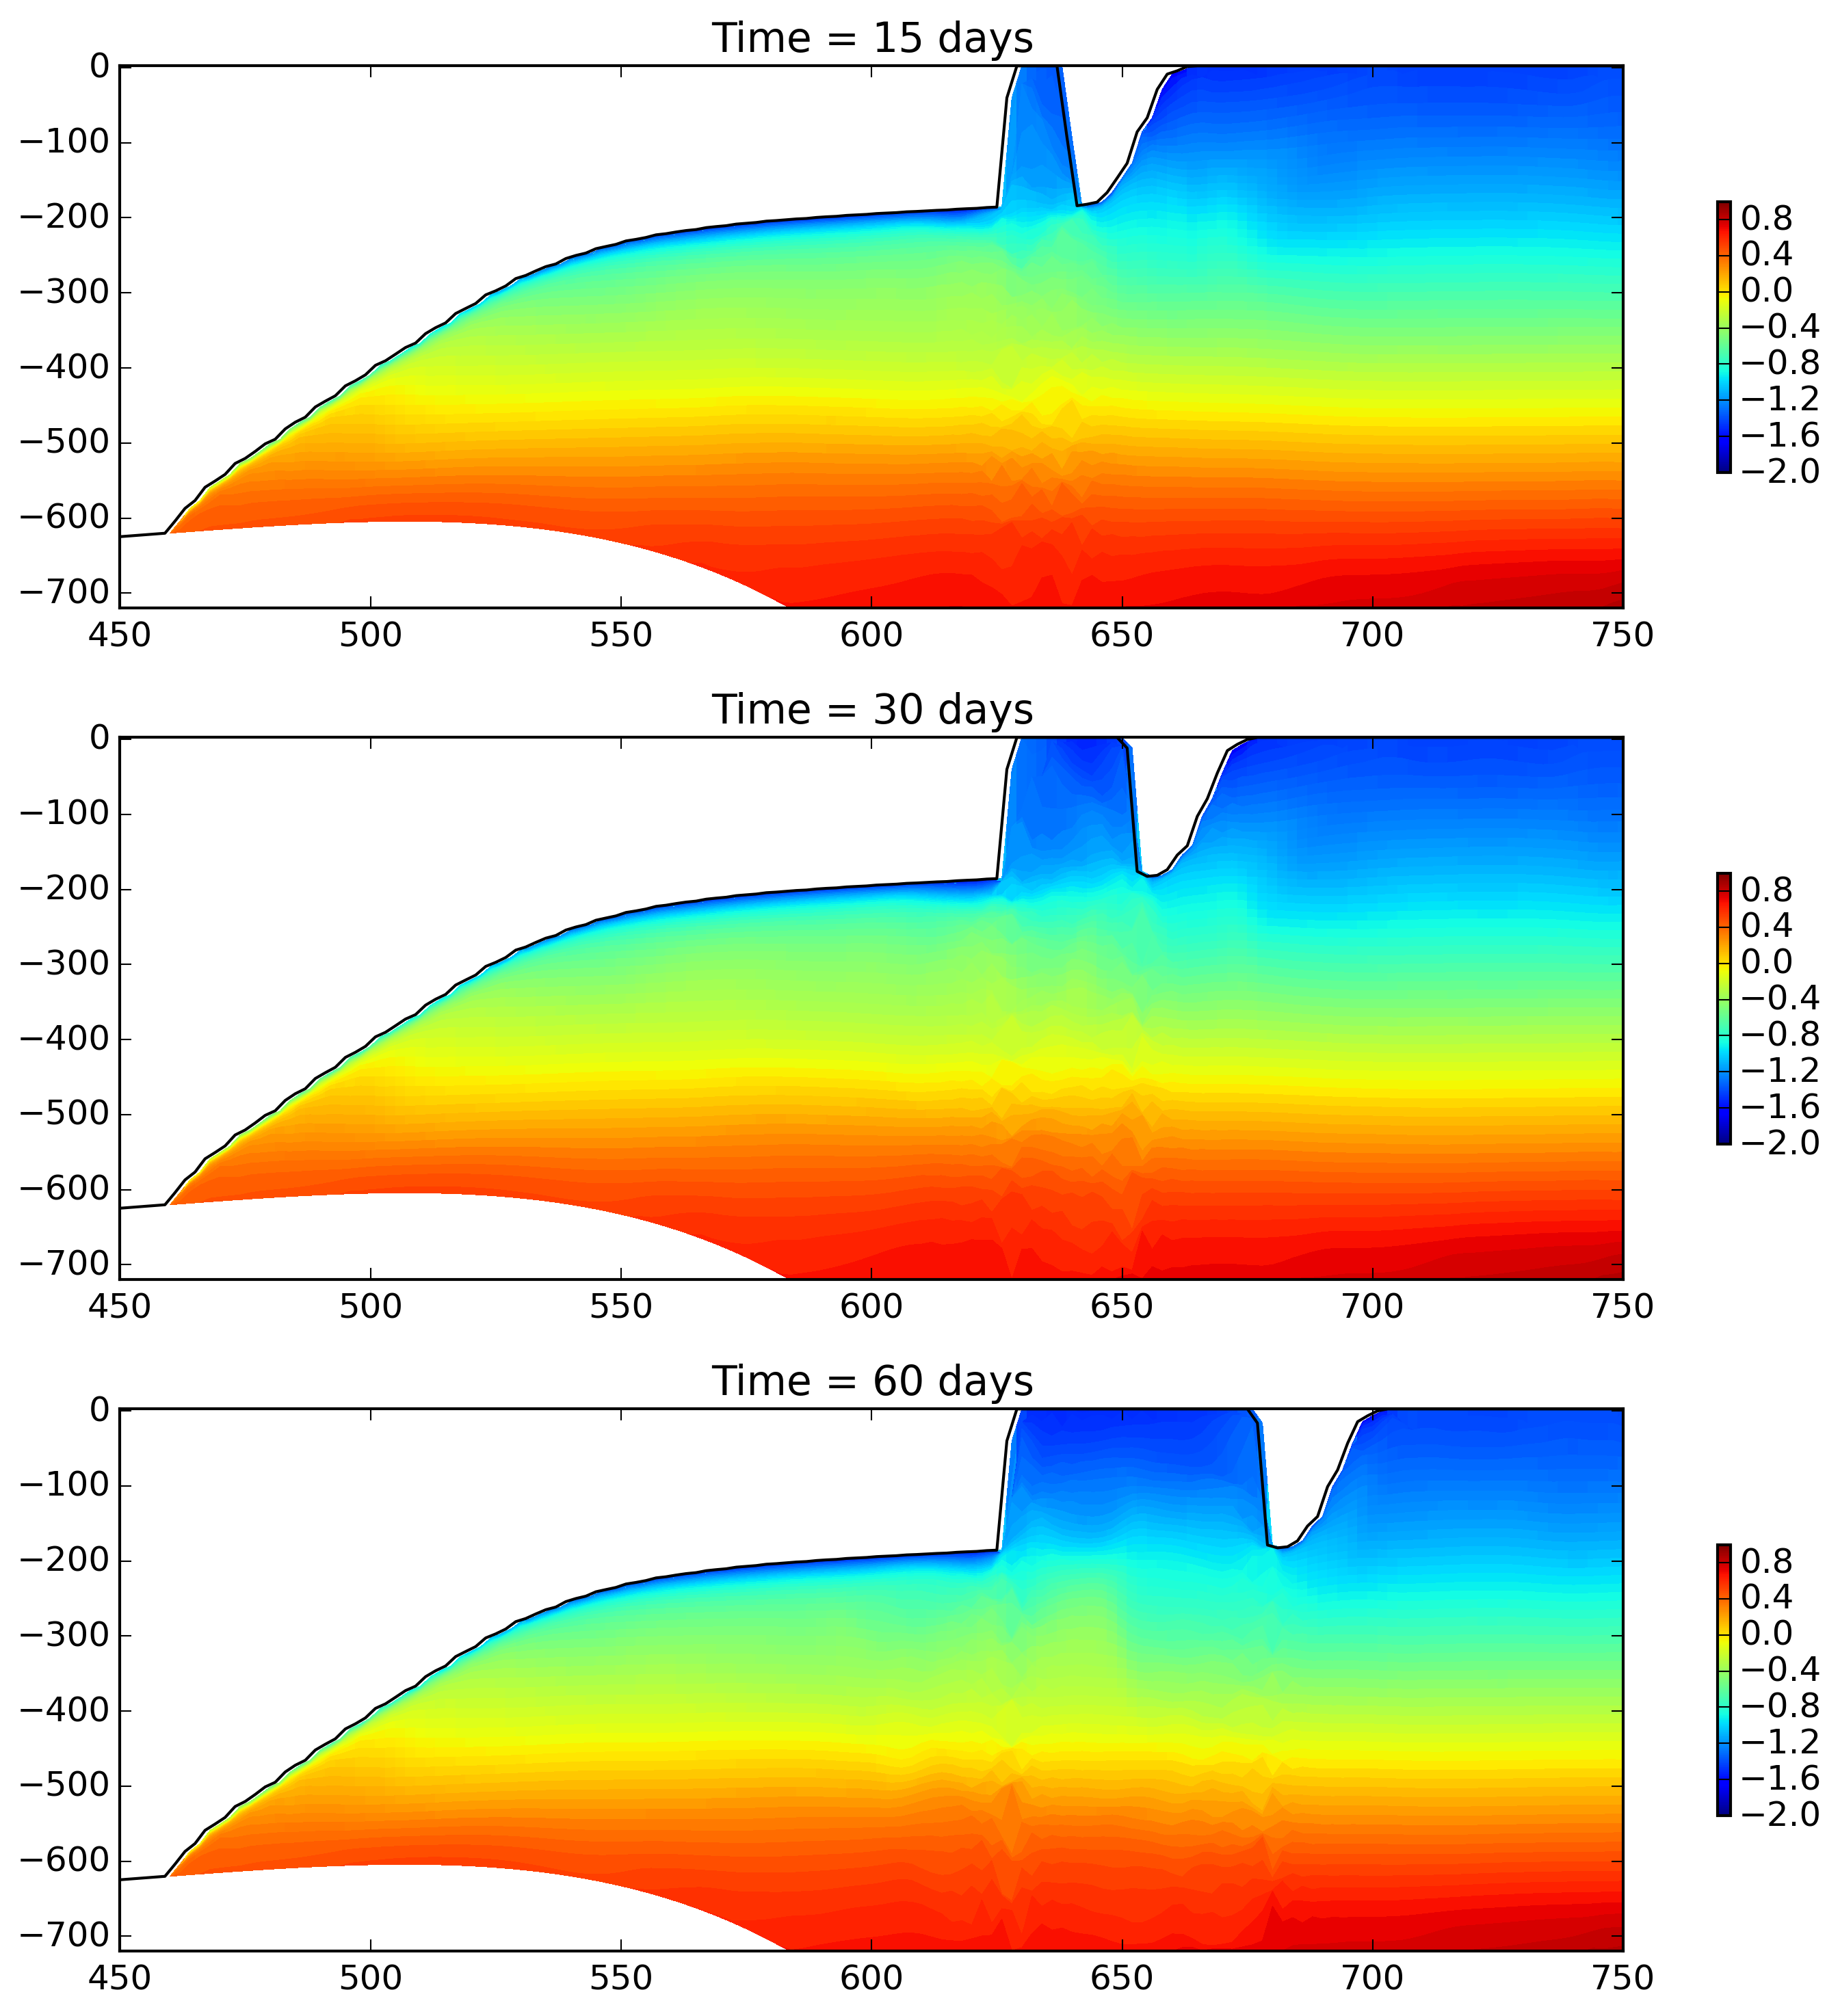
\includegraphics[width=0.99\textwidth]{/Users/alon/Desktop/files/Icebergs_clusters/Towards_Publication/Tech_paper/Github_stuff/Tech-paper/Figures/snapshots_after_melt_fixed_01_temp_layers}
\caption{ {Temperature section at $y=\frac{L_{y}}{2}$ for the tabular iceberg calving with fixed velocity simulation (using the LIISM ice shelf) at time (a) t=15, (b) t=30, and (c) t=60 days.}}
%FIgure created by \end{center}
\end{center}
\label{fig:Calving_fixed_side}
\end{figure}
  \clearpage



\begin{figure}
\begin{center}
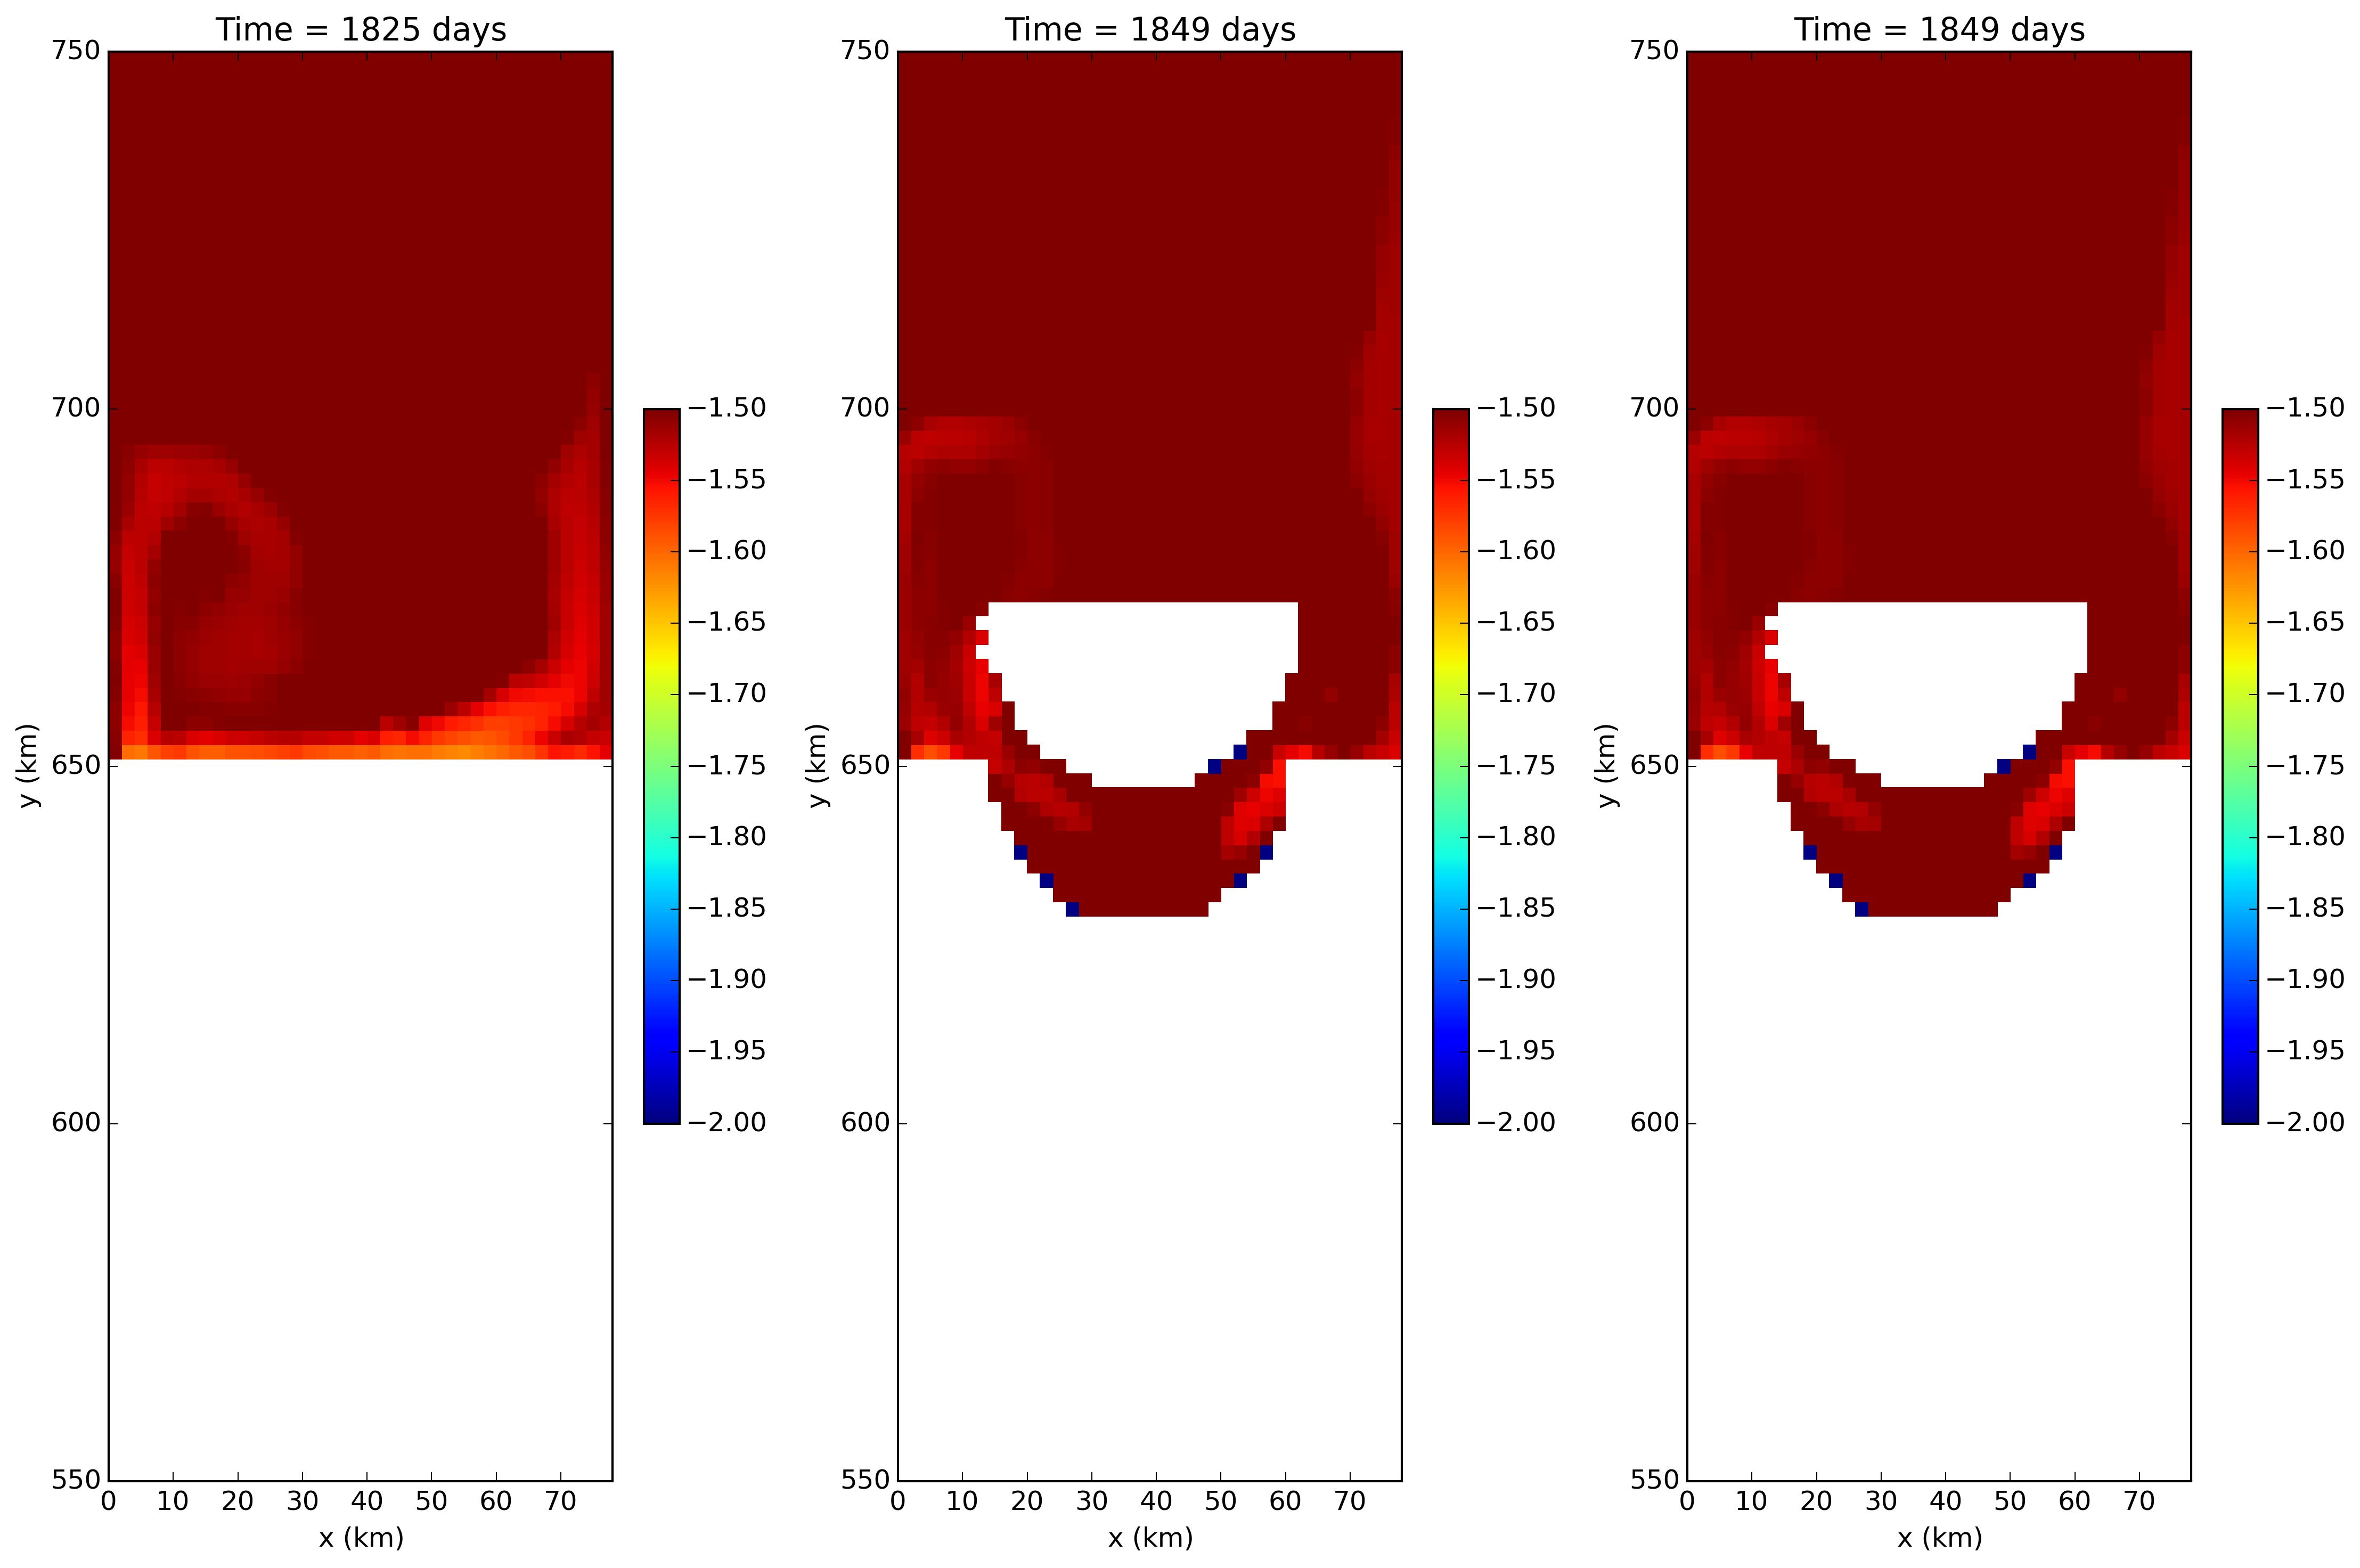
\includegraphics[width=0.99\textwidth]{/Users/alon/Desktop/files/Icebergs_clusters/Towards_Publication/Tech_paper/Github_stuff/Tech-paper/Figures/snapshots_after_melt_fixed_01_temp}
\caption{ {Sea surface temperature for the tabular iceberg calving with fixed velocity simulation at time (a) t=15, (b) t=30, and (c) t=60 days.}}
\end{center}
%FIgure created by \end{center}
\label{fig:Calving_fixed_top}
\end{figure}
 \clearpage



%\begin{figure}
%\begin{center}
%\includegraphics[width=0.99\textwidth]{/Users/alon/Desktop/files/Icebergs_clusters/Towards_Publication/Tech_paper/Github_stuff/Tech-paper/Diagrams/Interactive forces.pdf}
%\caption{ {Schematic of interactive forces}}
%\end{center}
%FIgure created by \end{center}
%\label{fig:Interactive_forces}
%\end{figure}
 %\clearpage



\begin{figure}
\begin{center}
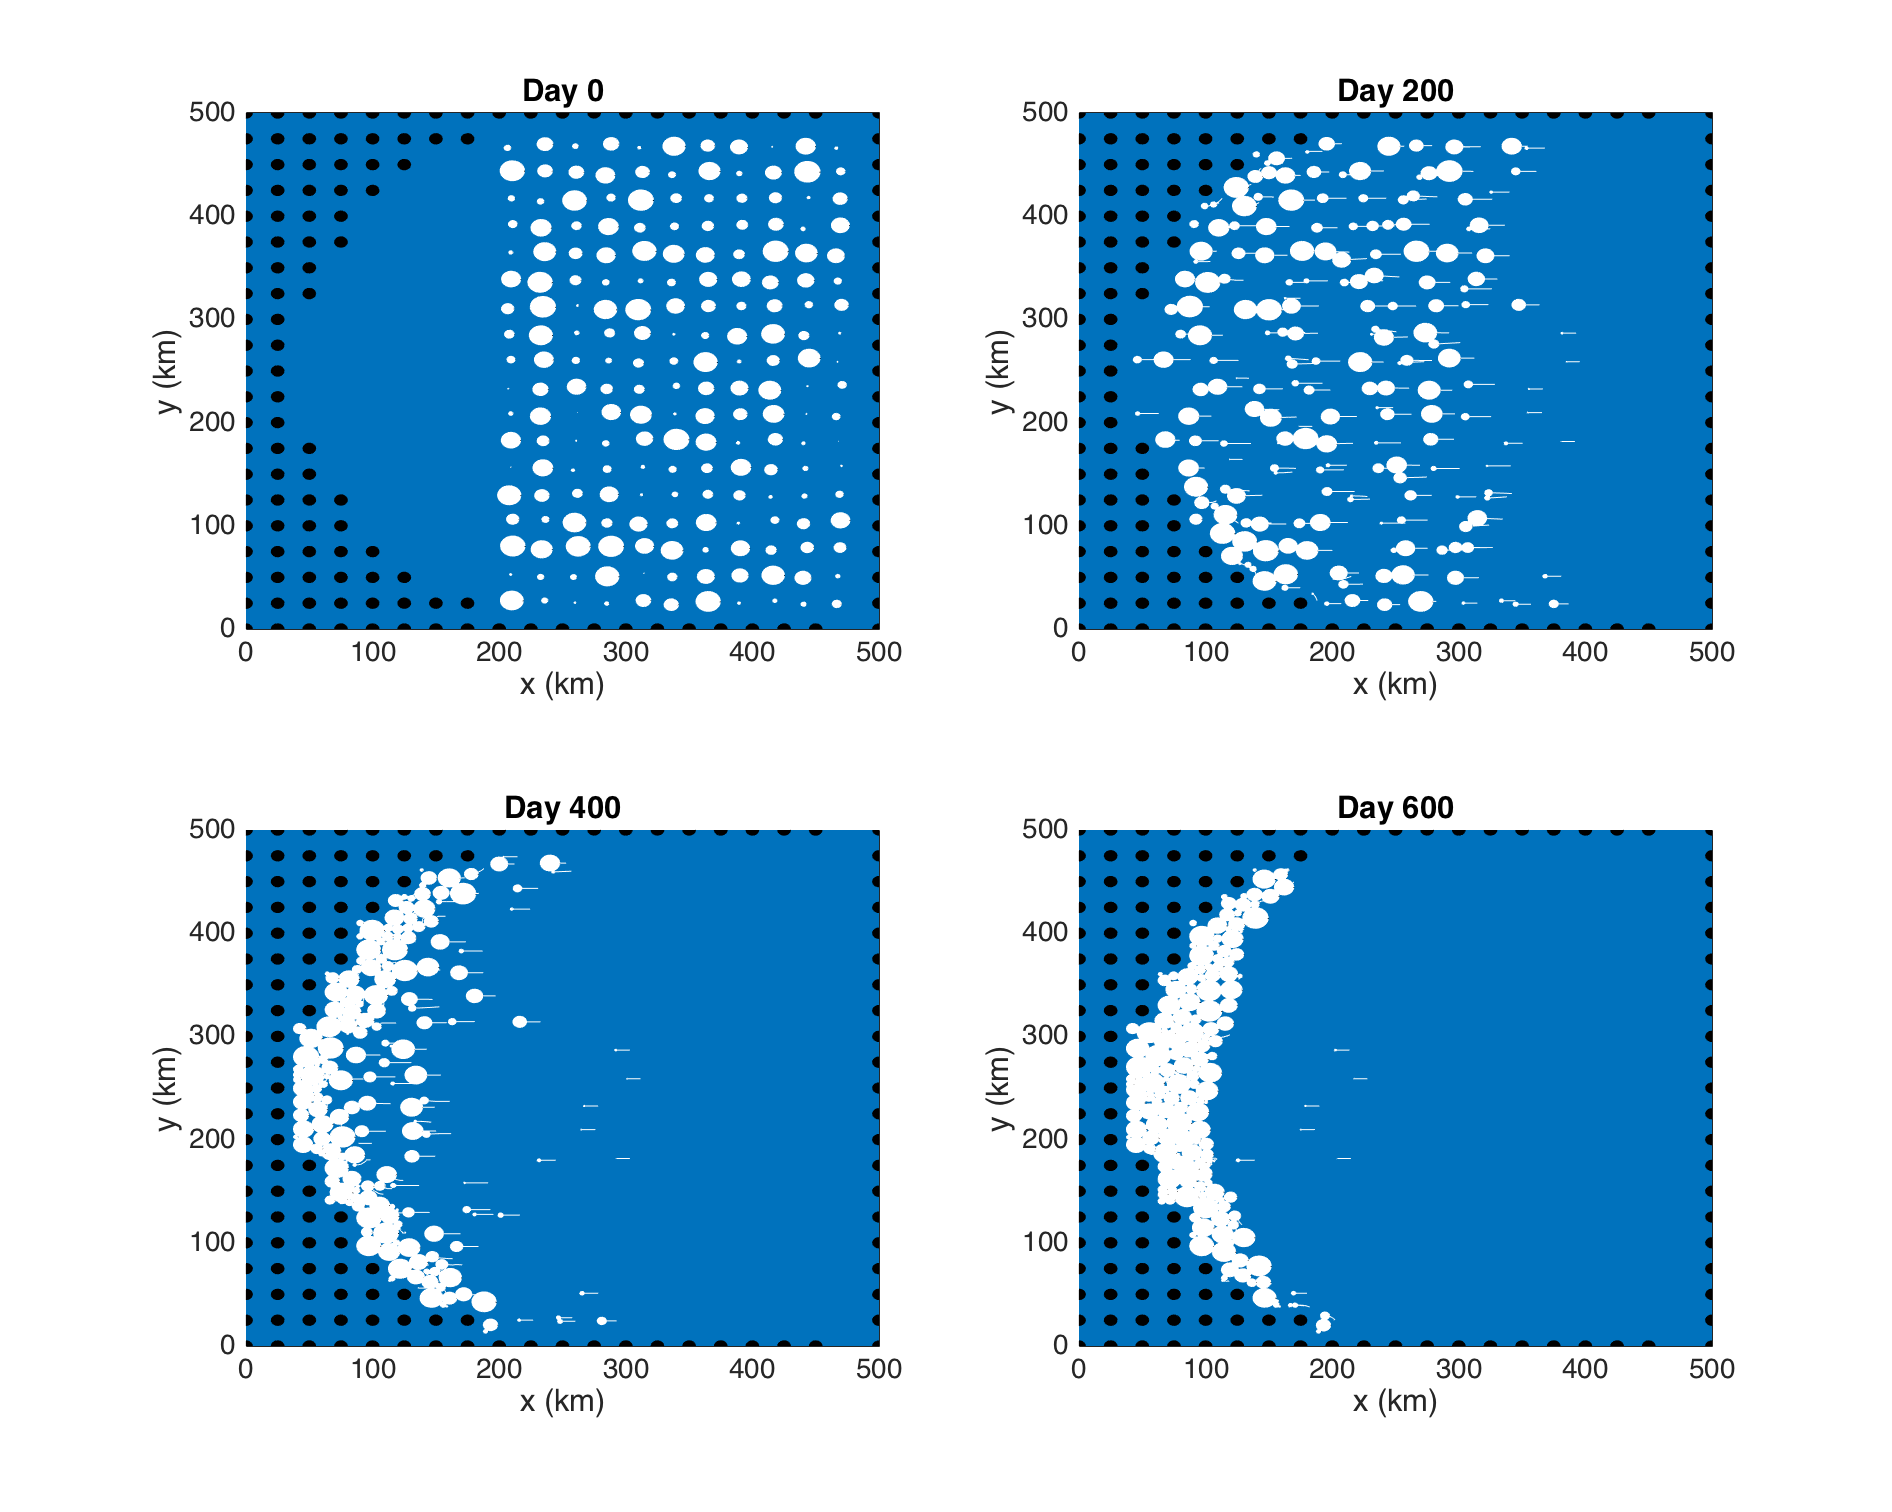
\includegraphics[width=0.99\textwidth]{/Users/alon/Desktop/files/Icebergs_clusters/Towards_Publication/Tech_paper/Github_stuff/Tech-paper/Figures/Regular_towards_coast}
\caption{ {Positions of ice elements at time t=0, 200, 400, 600 days for the simulation. The size of the dots shows the surface area (and interaction diameter) of each ice element. Land points are shown by black circles. }}
\end{center}
%FIgure created by \end{center}
\label{fig:Regular_Uncoupled_sim}
\end{figure}
 \clearpage




\begin{figure}
\begin{center}
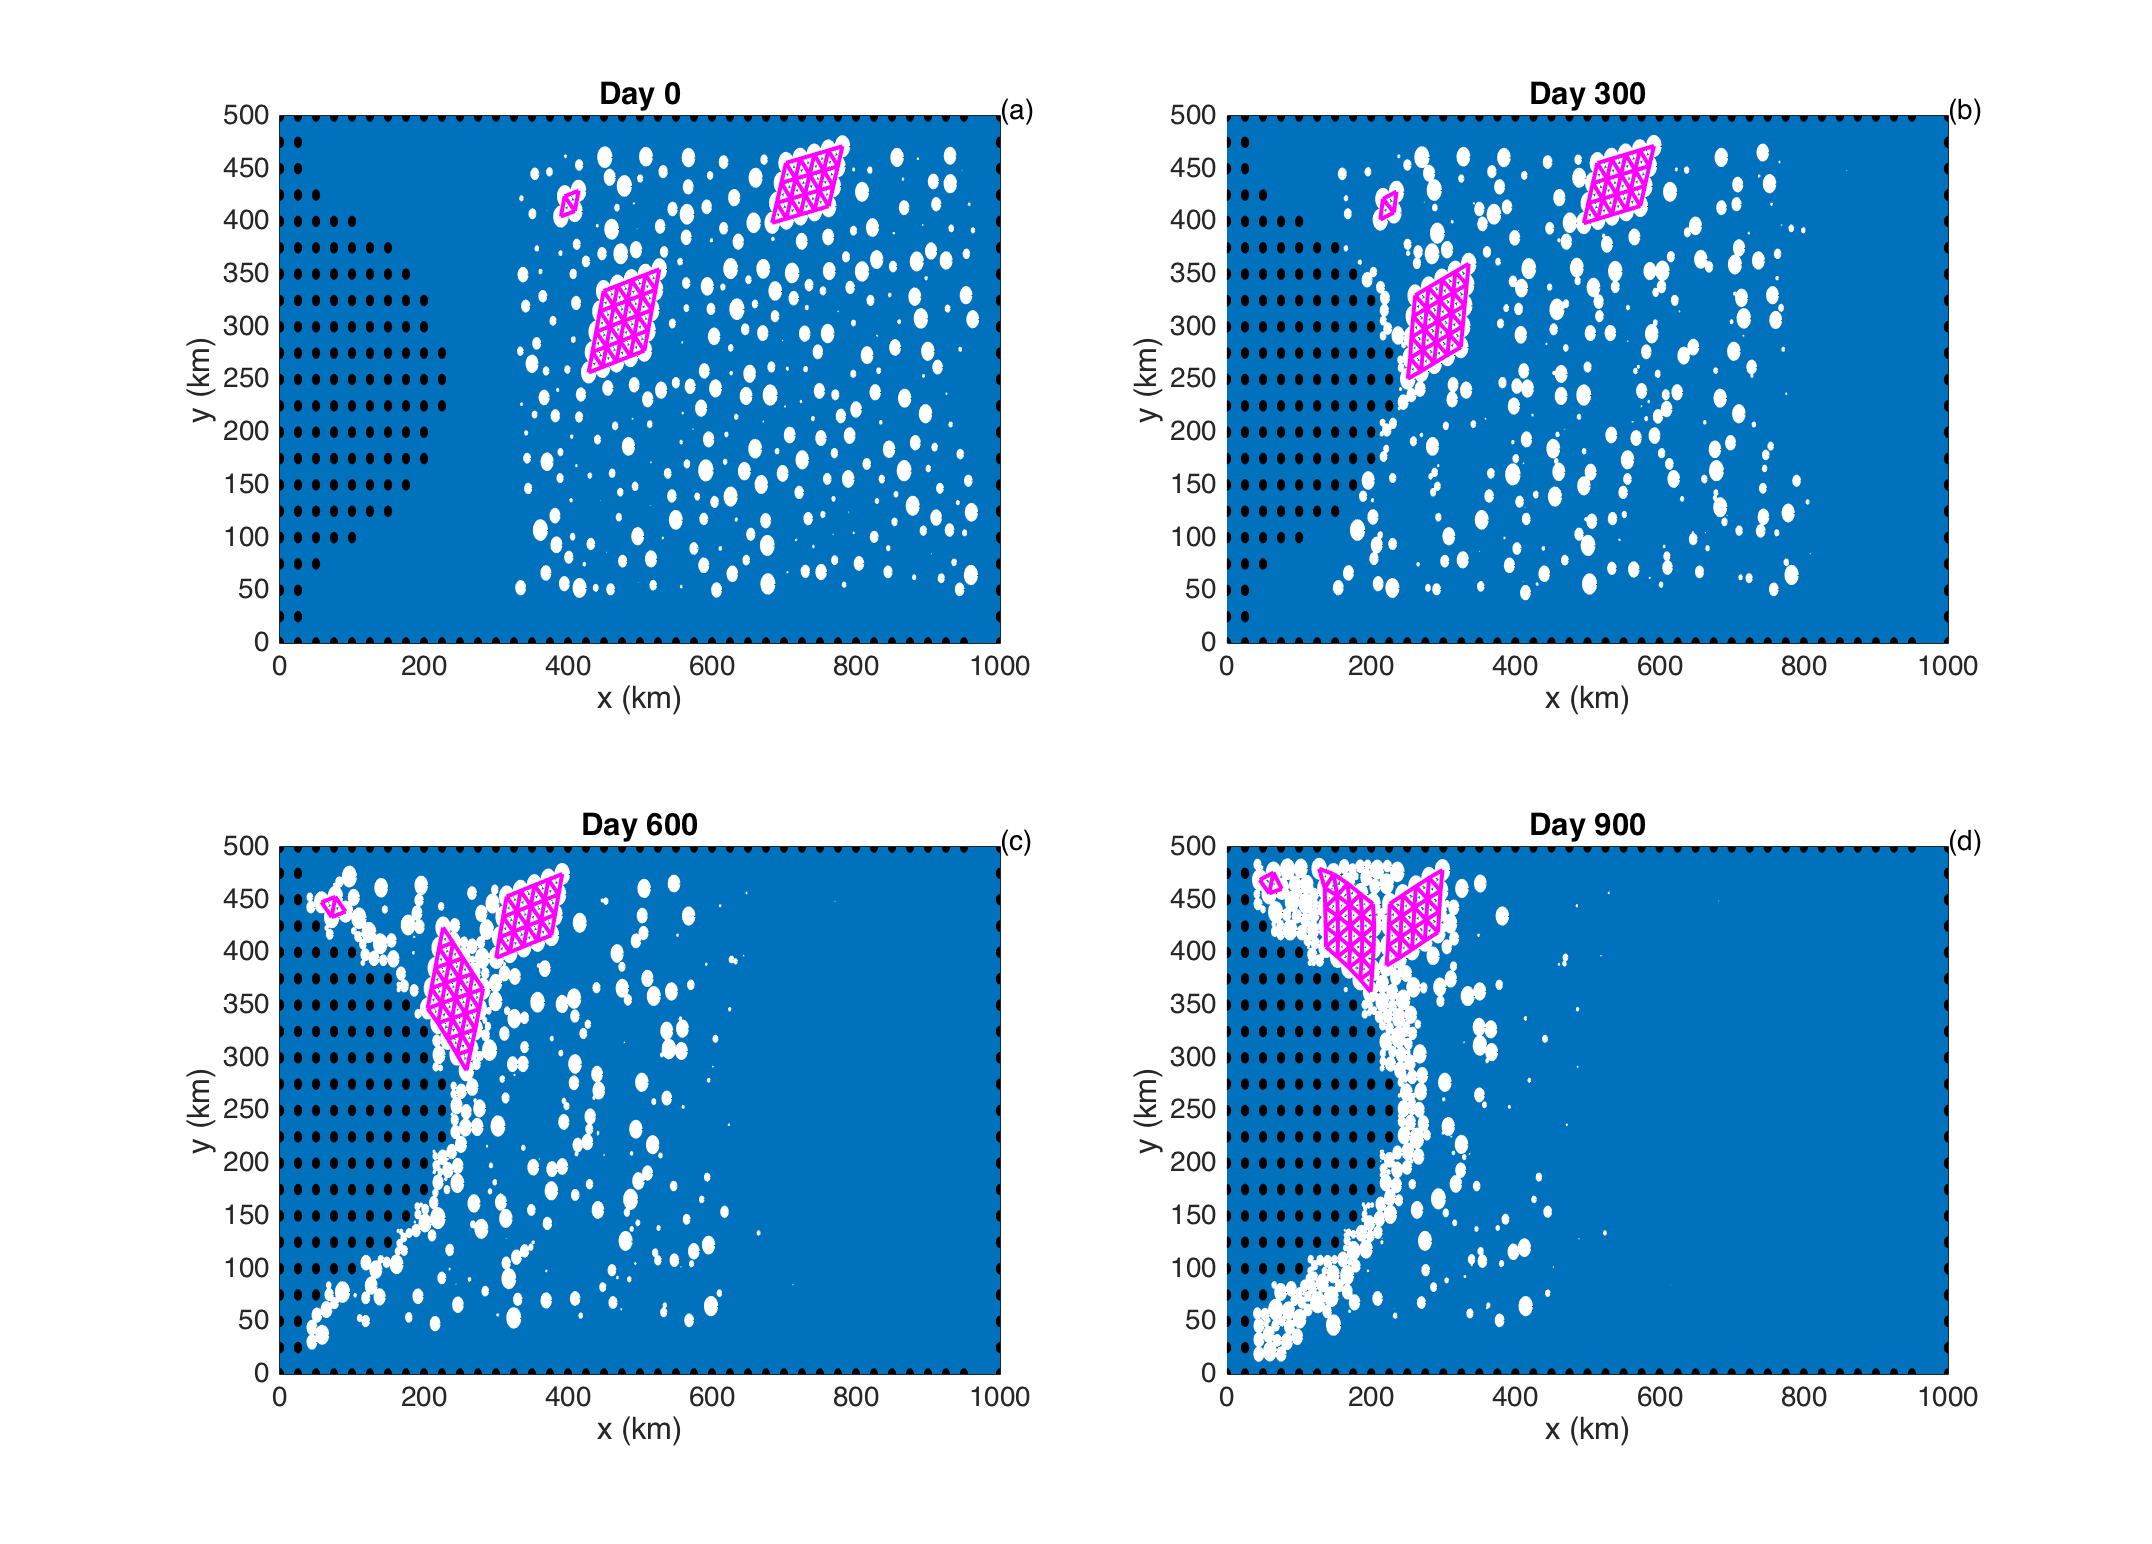
\includegraphics[width=0.99\textwidth]{/Users/alon/Desktop/files/Icebergs_clusters/Towards_Publication/Tech_paper/Github_stuff/Tech-paper/Figures/Tabular_and_regular_towards_coast_manual}
\caption{ {Positions of ice elements at time t=0, 300, 600, 900 days for the simulation. The size of the dots shows the surface area (and interaction diameter) of each ice element. Bonds between ice elements are plotted in magenta. Three tabular icebergs are shown, with 25, 16 and 4 elements respectively. Land points are shown by black circles. }}
\end{center}
%FIgure created by \end{center}
\label{fig:Uncoupled_sim}
\end{figure}
 \clearpage




\begin{figure}
\begin{center}
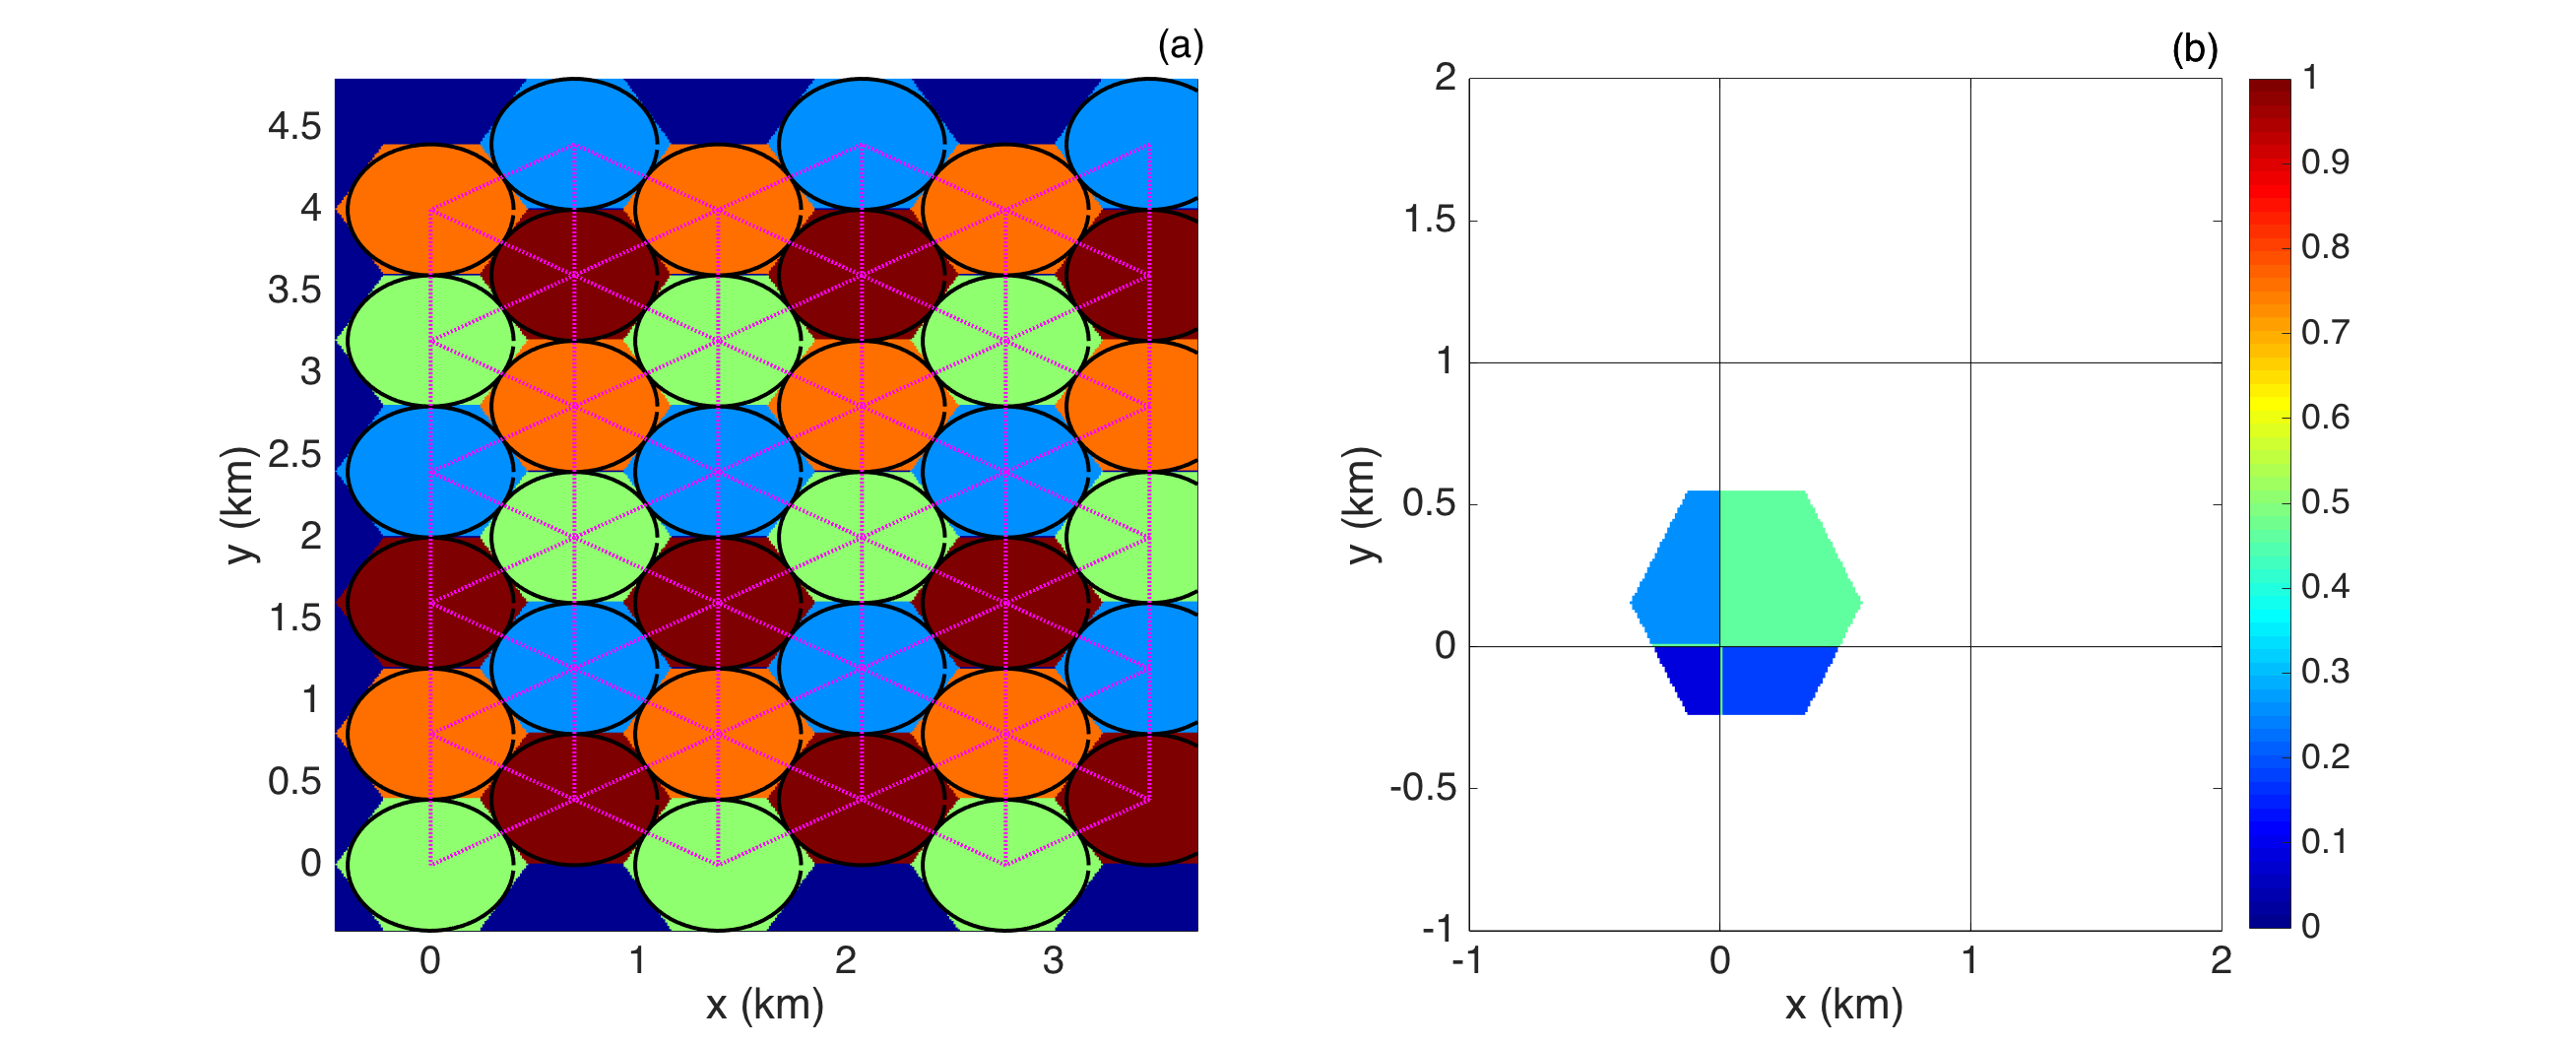
\includegraphics[width=0.99\textwidth]{/Users/alon/Desktop/files/Icebergs_clusters/Towards_Publication/Tech_paper/Github_stuff/Tech-paper/Figures/hex_intersecting_rectangles}
\caption{ {(a) Intersection of hexagonal element and ocean grid is used to find weights to spread LIISM properties to the ocean grid. (b) Hexagonal elements are initialized in a staggered lattice as shown. Adjacent elements are bonded together. The centers of bonded elements are plotted in pink. The element bonds form equilateral triangles which give the larger structure rigidity. The black circles shows to the interactive length scales used in element interactions.}}
\end{center}
%FIgure created by \end{center}
\label{fig:Hex_intersections}
\end{figure}
 \clearpage




\begin{figure}
\begin{center}
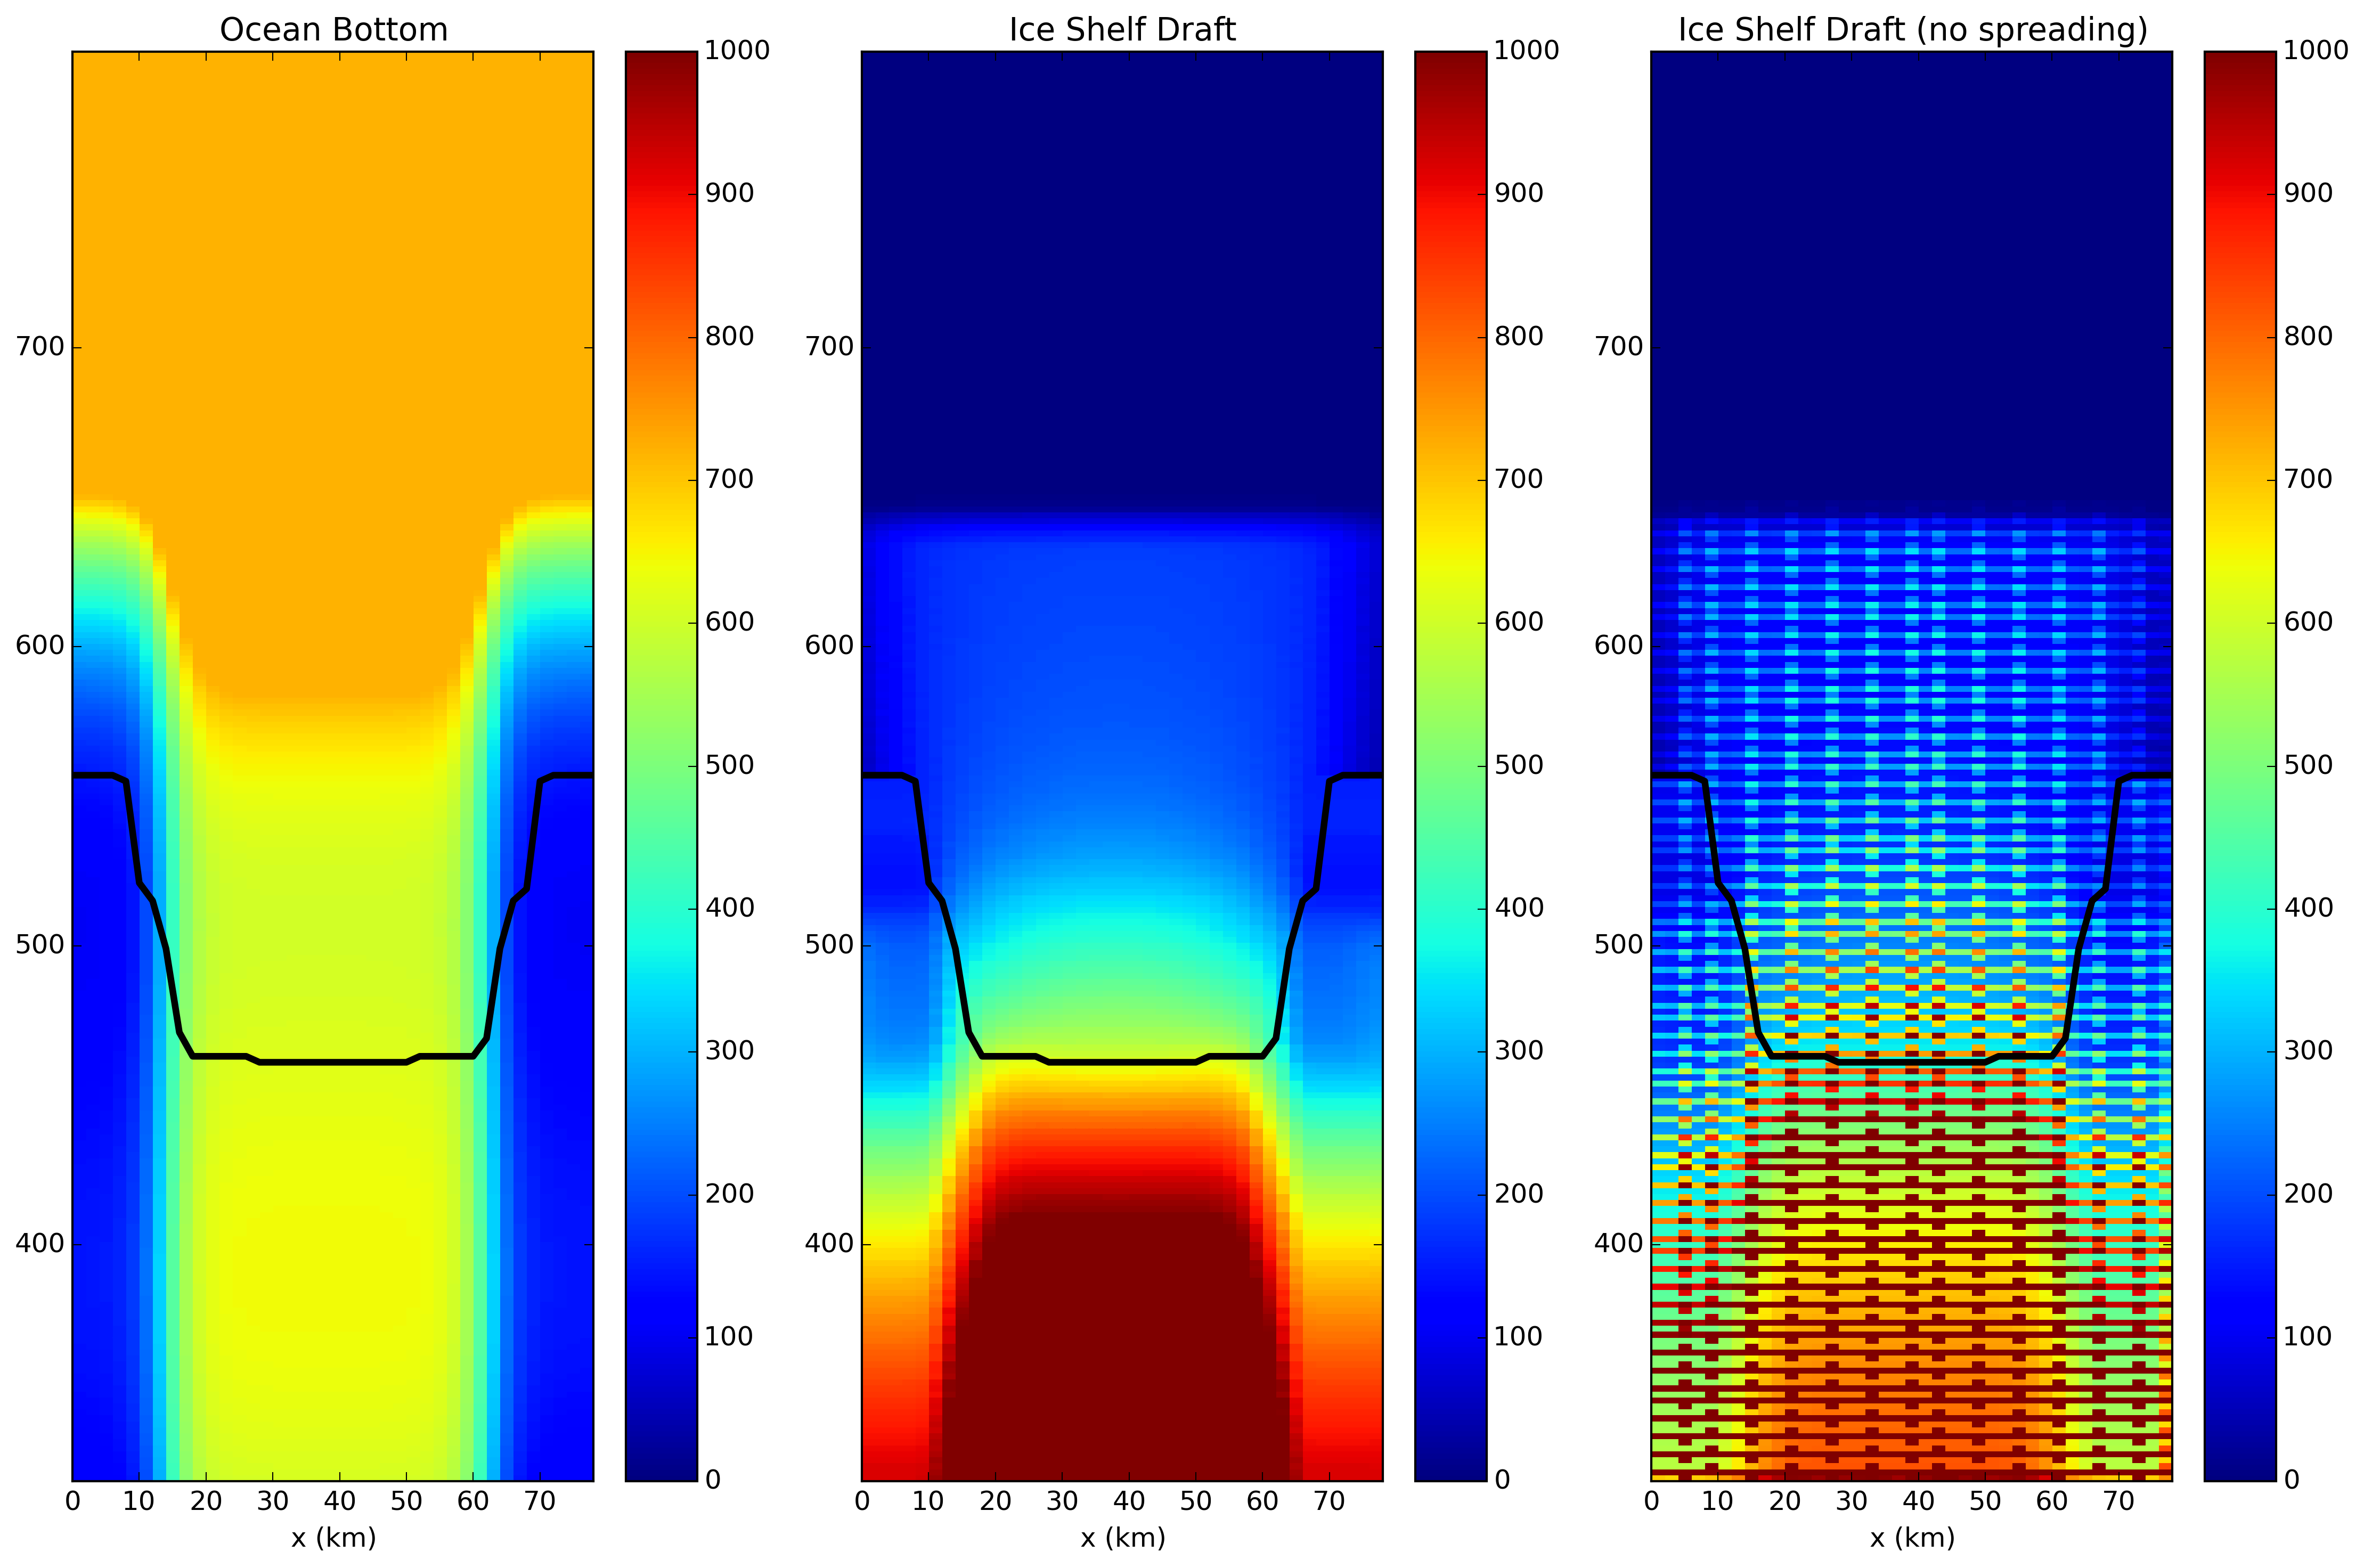
\includegraphics[width=0.99\textwidth]{/Users/alon/Desktop/files/Icebergs_clusters/Towards_Publication/Tech_paper/Github_stuff/Tech-paper/Figures/static_shelf_solo_D_spread_mass_mass.png}
\caption{ {(a) Ocean bottom topography in ISOMIP configuration. (b) Ice shelf draft used in static shelf experiment. The ice draft is calculated from the ice mass in an ocean grid cell, which is found by spreading ice mass across ocean cells accounting for the size of each element (as explained in Section ?). (c) Same as in panel (b), except that the interpolation does not account for iceberg size, and instead treats elements as point masses.}}
\end{center}
%FIgure created by \end{center}
\label{fig:ISOMIP_exp}
\end{figure}
 \clearpage
 
 
 
\begin{figure}
\begin{center}
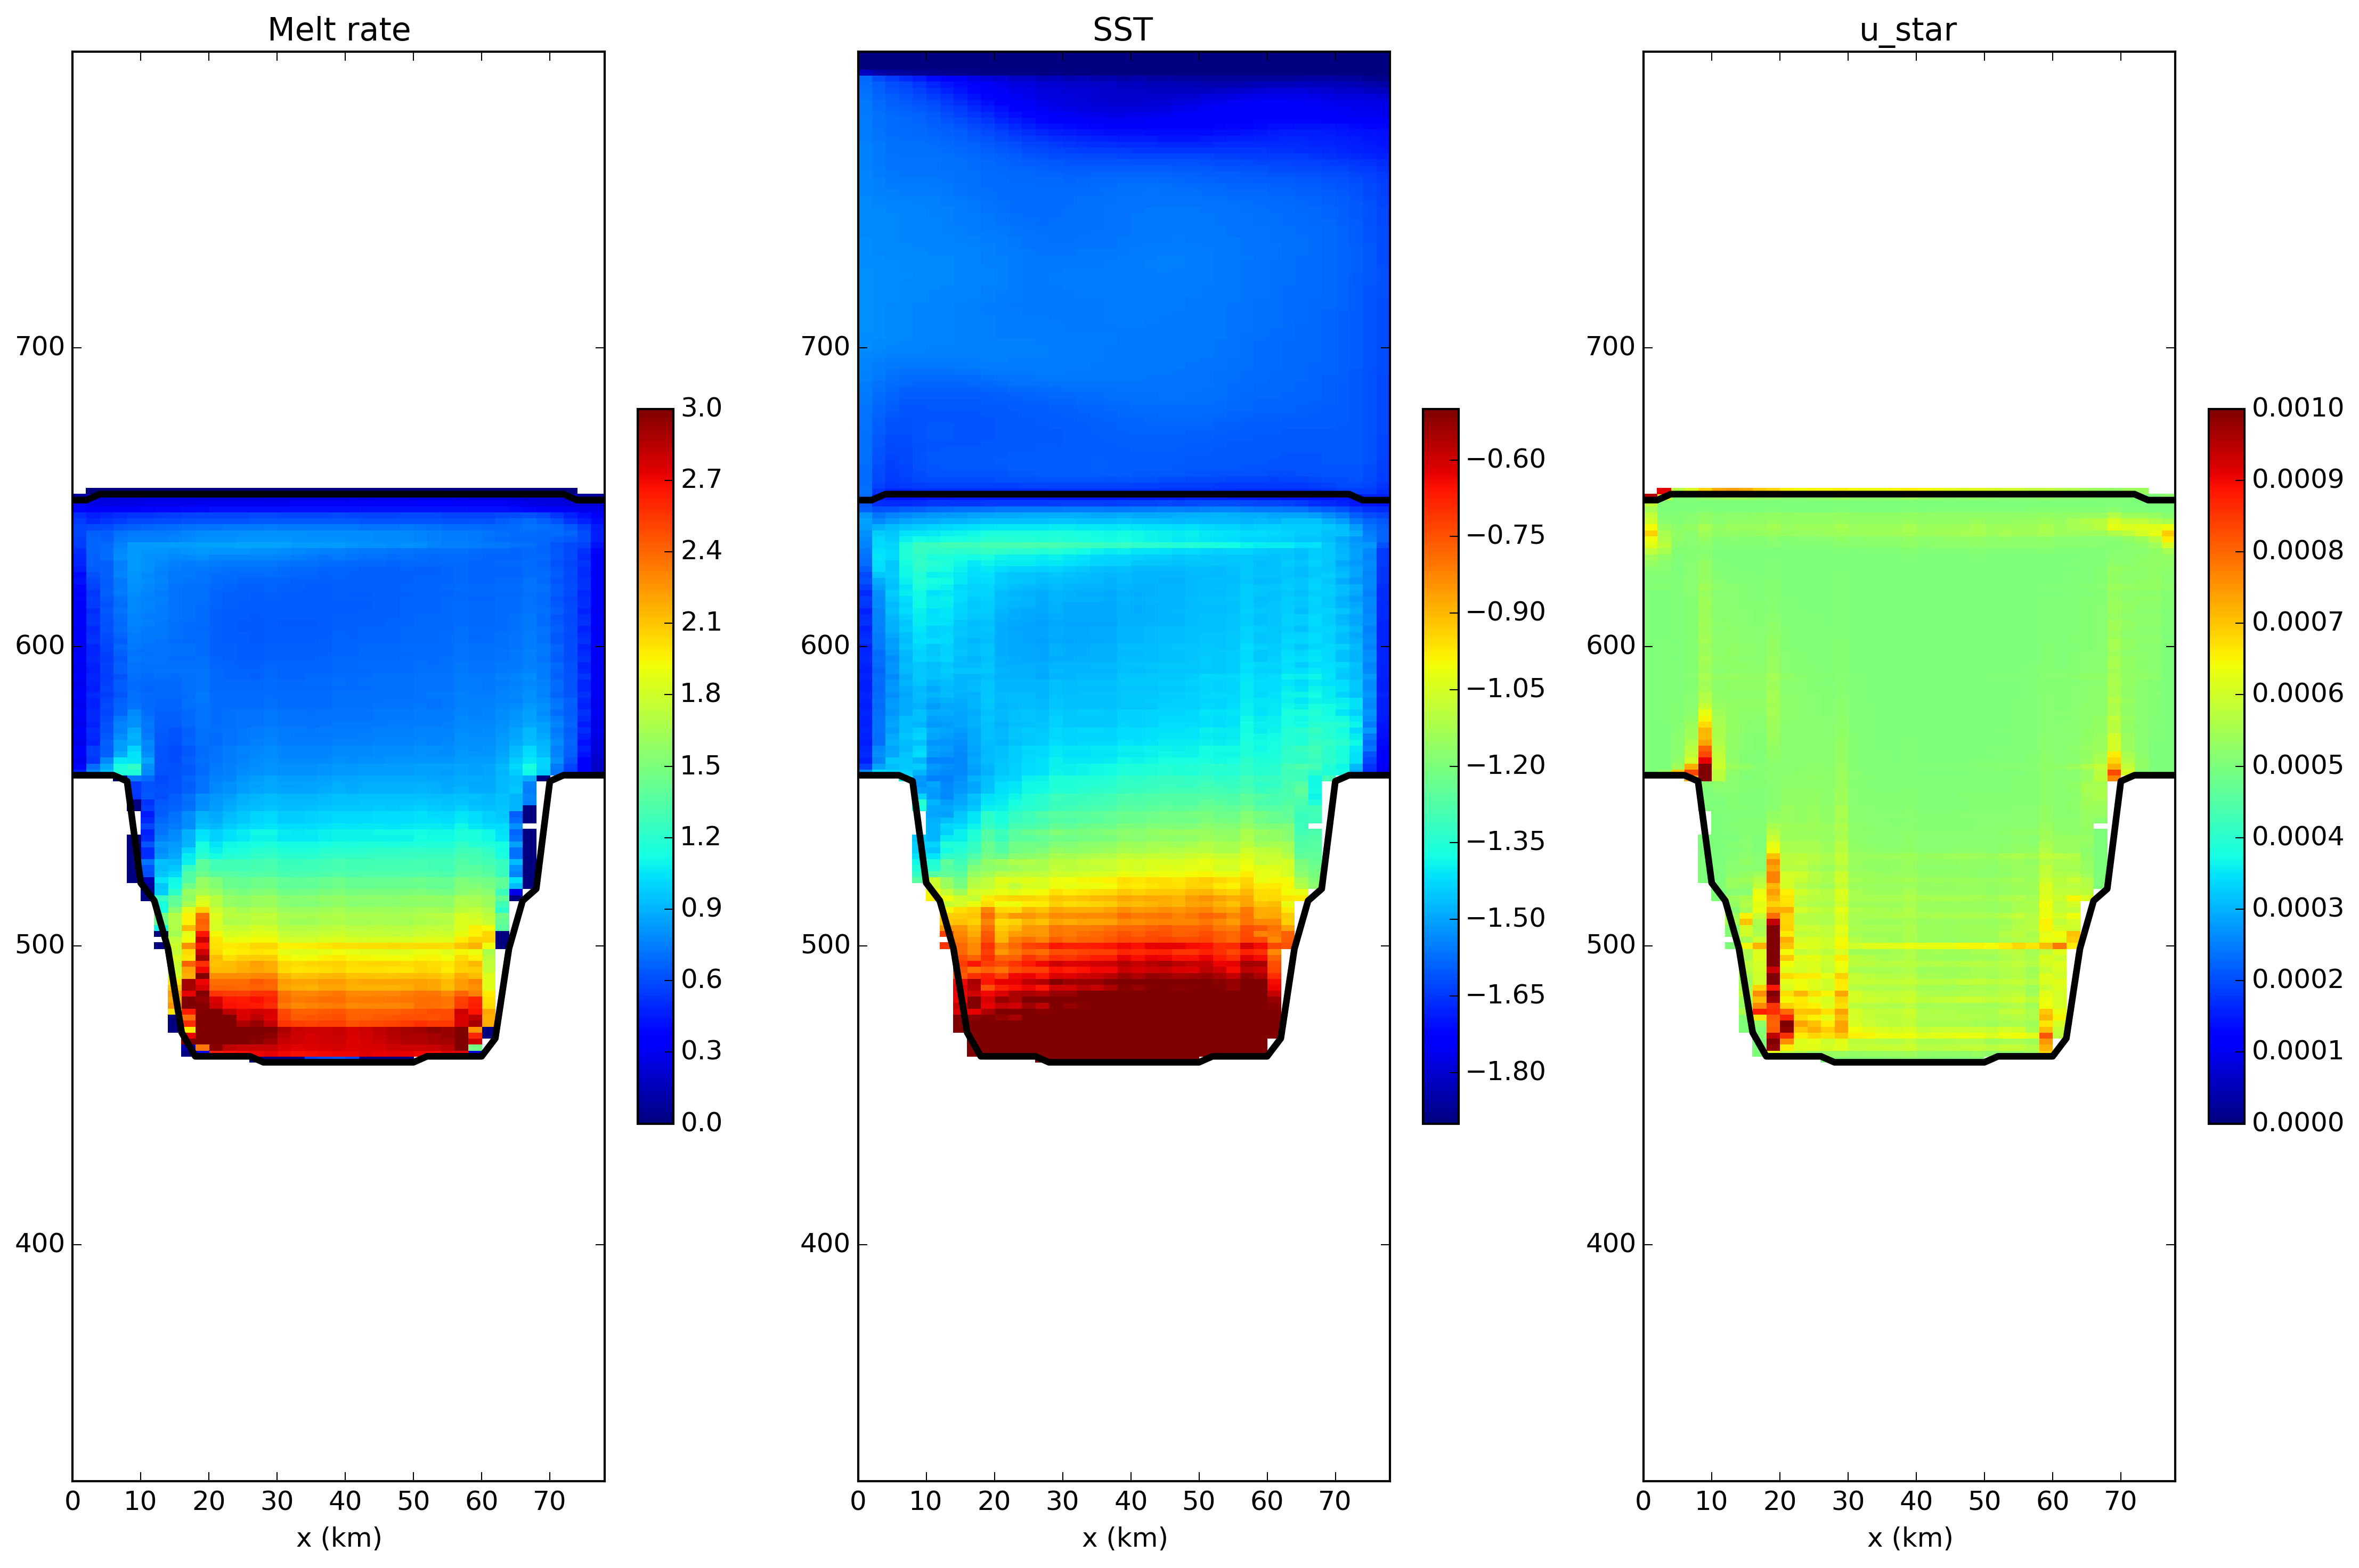
\includegraphics[width=0.99\textwidth]{/Users/alon/Desktop/files/Icebergs_clusters/Towards_Publication/Tech_paper/Github_stuff/Tech-paper/Figures/static_shelf_solo_melt_m_per_year_sst_ustar_iceberg.png}
\caption{ {Results of the static ice shelf experiment using the LIISM model. The three panels show 5 year time average of the (a) melt rate, (b) ocean surface temperature and (c) $u^{*}$  in the top layer of the simulation (at the surface or directly below the ice shelf).}}
\end{center}
%FIgure created by \end{center}
\label{fig:static_solo_melt}
\end{figure} 
 \clearpage
 




\begin{figure}
\begin{center}
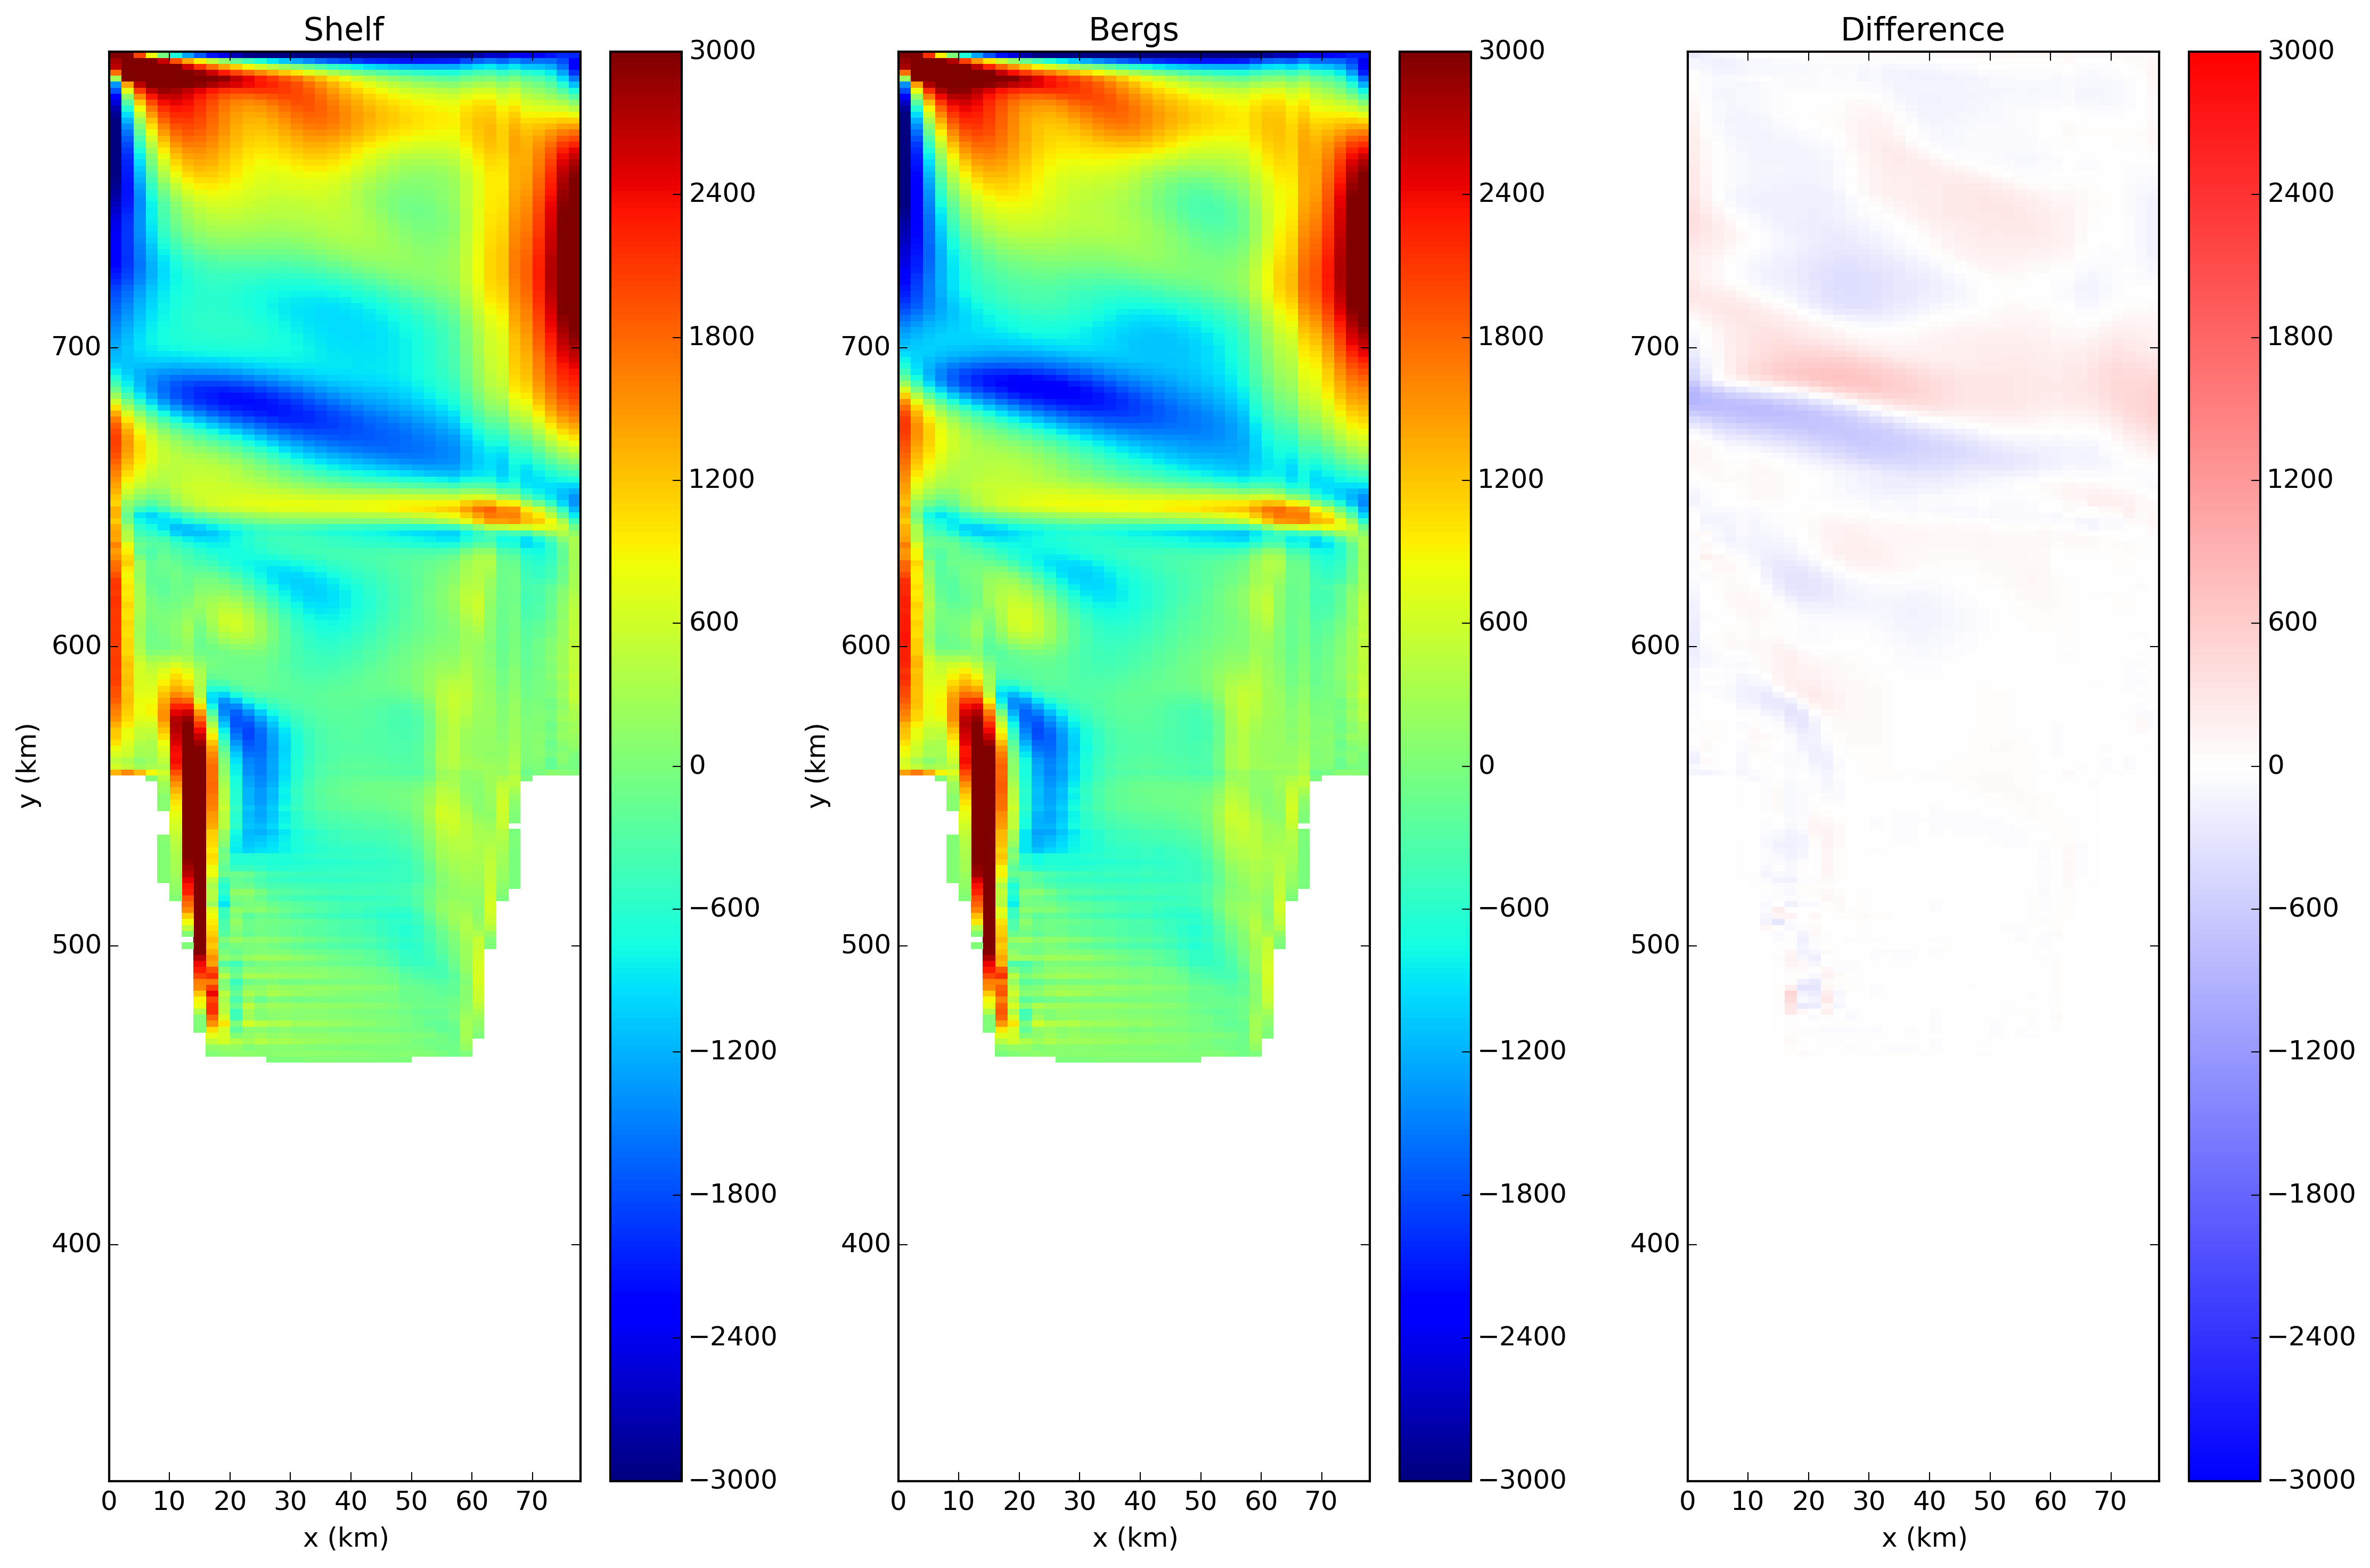
\includegraphics[width=0.99\textwidth]{/Users/alon/Desktop/files/Icebergs_clusters/Towards_Publication/Tech_paper/Github_stuff/Tech-paper/Figures/static_shelf_comparison_barotropic_sf.png}
\caption{ {Comparison of Eulerian ice shelf model and Lagrangian Ice shelf model barotropic stream function}}
\end{center}
%FIgure created by \end{center}
\label{fig:Bt_comparison}
\end{figure}
 \clearpage


 


%\begin{figure}
%\begin{center}
%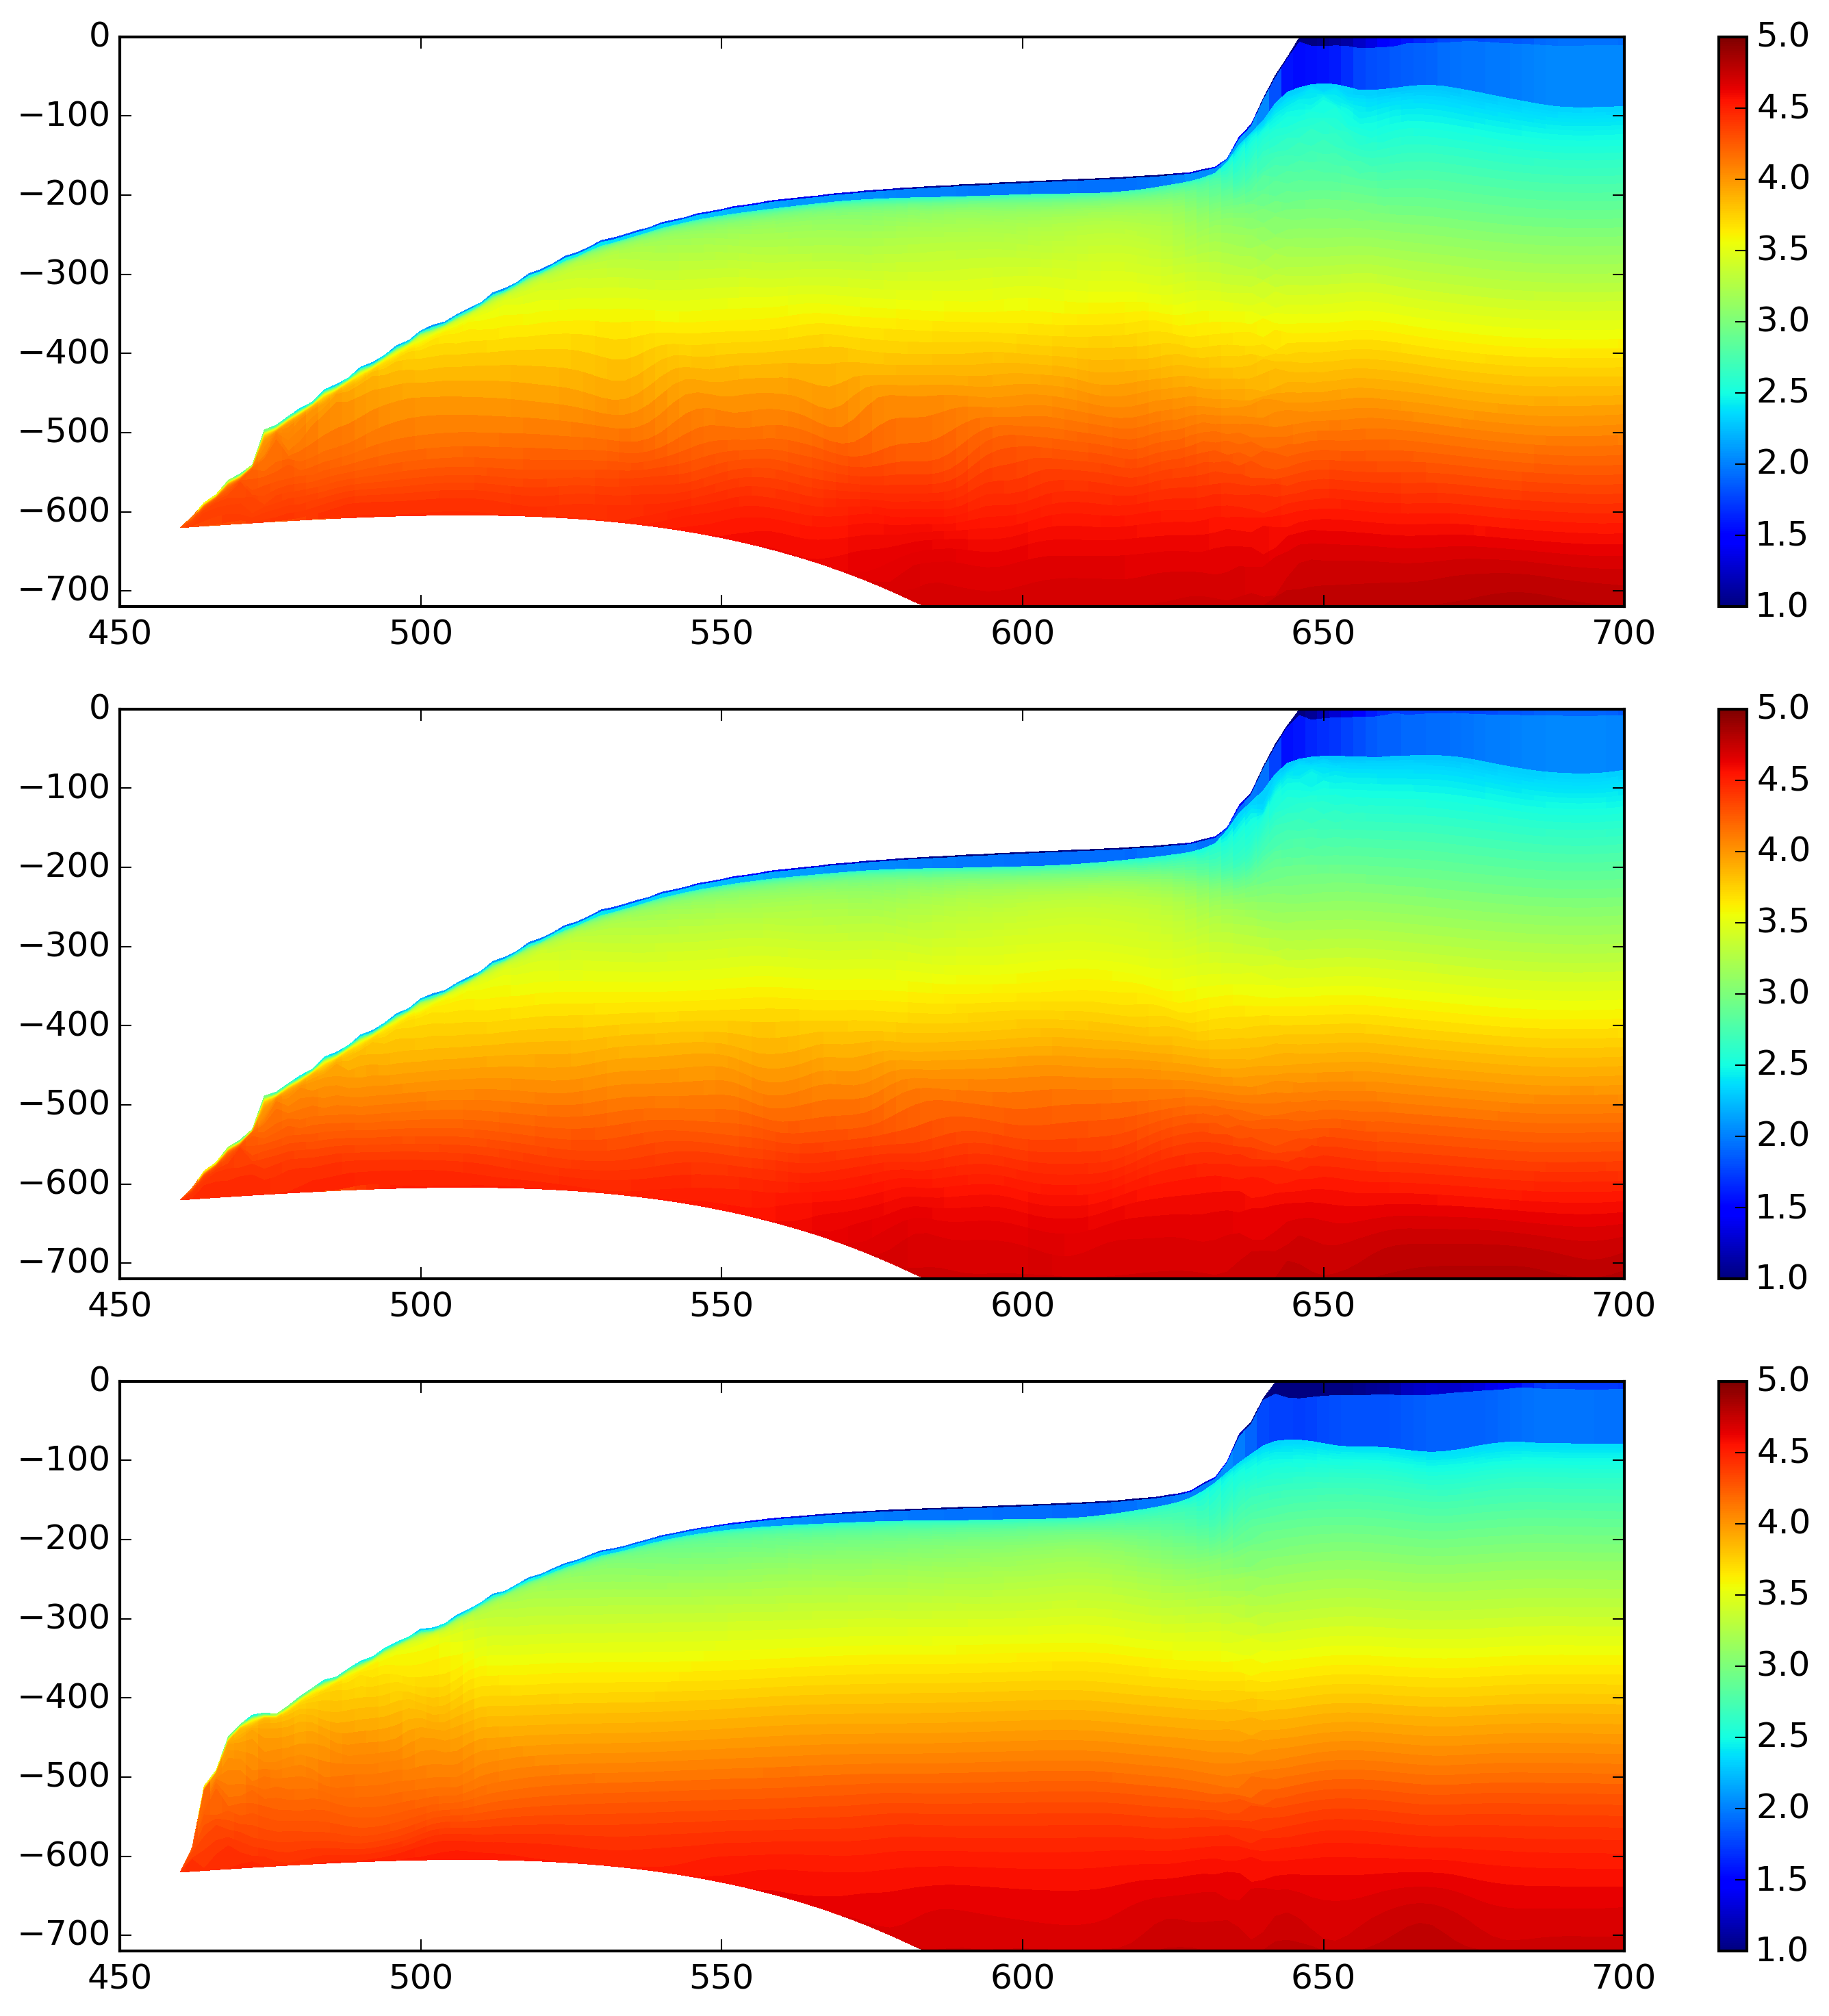
\includegraphics[width=0.99\textwidth]{/Users/alon/Desktop/files/Icebergs_clusters/Towards_Publication/Tech_paper/Github_stuff/Tech-paper/Figures/melting_shelf_temp_layers.png}
%\caption{ {Temperature section at $y=\frac{L_{y}}{2}$ for the decaying ice shelf simulation (using the LIISM ice shelf) at time (a) t=0, (b) t=100(?), (c) t=200 days. As the ice shelf melts, it decays and the pressure at the ocean surface decreases. }}
%\end{center}
%FIgure created by \end{center}
%\label{fig:Decaying_shelf}
%\end{figure}

%\clearpage


\begin{figure}
\begin{center}
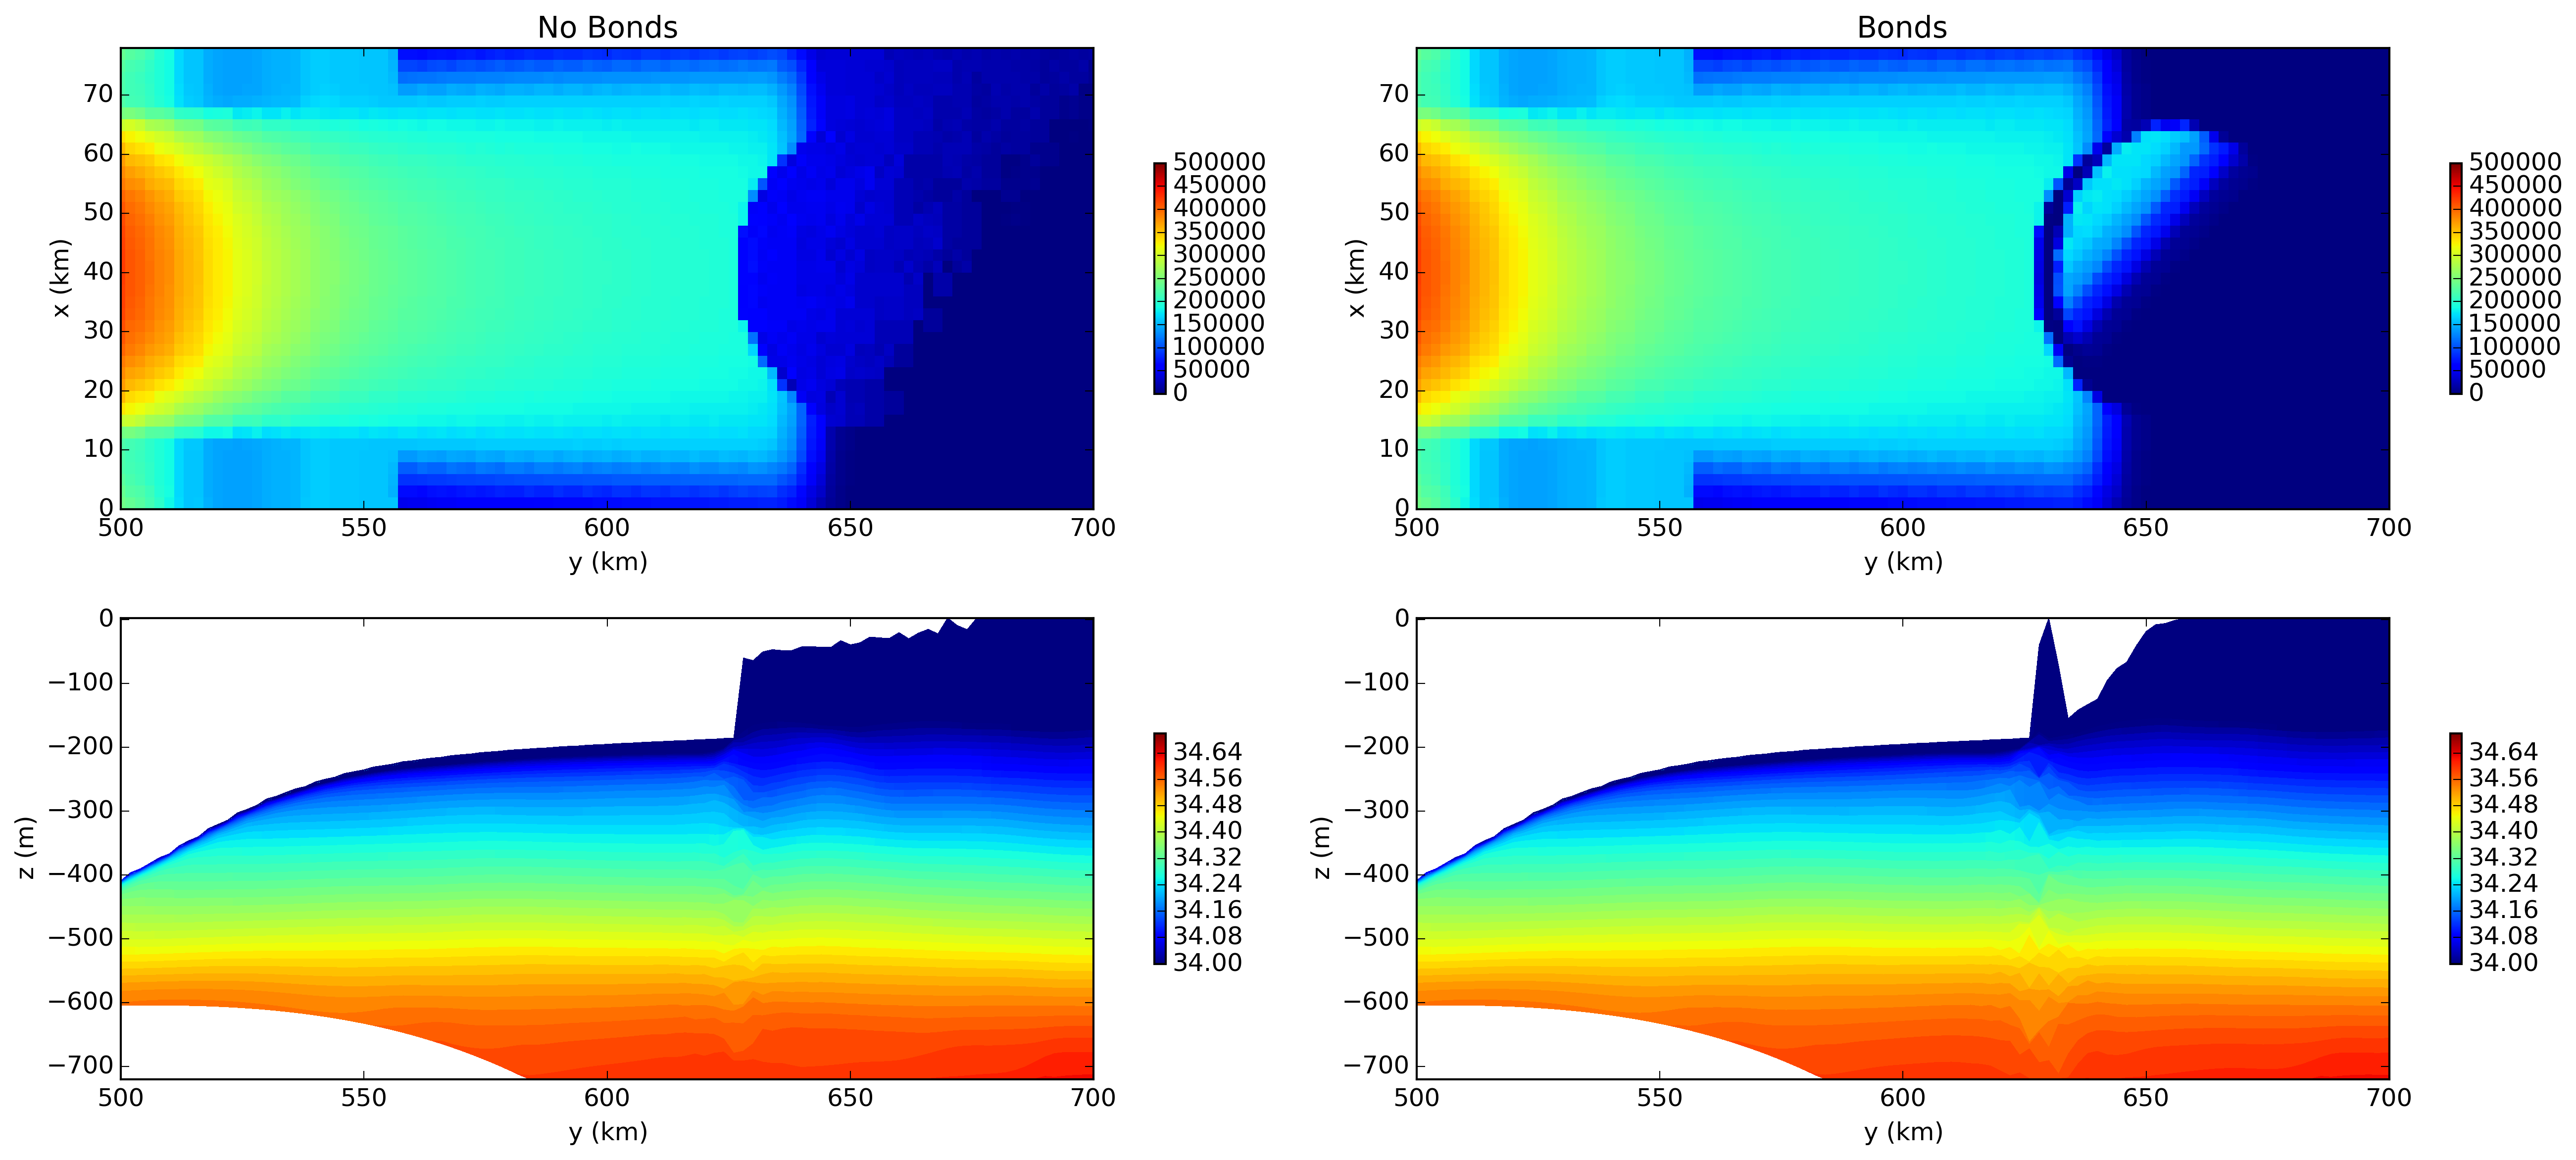
\includegraphics[width=0.99\textwidth]{/Users/alon/Desktop/files/Icebergs_clusters/Towards_Publication/Tech_paper/Github_stuff/Tech-paper/Figures/drift_bond_salt_layers.png}
\caption{ {Calving of tabular iceberg with the LIISM model fully coupled to the ocean for simulations with and without bonds between ice elements. The top row show the aveage draft of ice above the ocean in each grid cell for the simulation (a) with and (b) without bonds. The bottom row shows the corresponding temperature section at $y=\frac{L_{y}}{2}$ for the simulation (a) with and (b) without bonds.  All snapshots are taken at time t= 30 days.}}
\end{center}
%FIgure created by \end{center}
\label{fig:Bond_vs_No_bond}
\end{figure}


 
  \clearpage



%\begin{figure}
%\begin{center}
%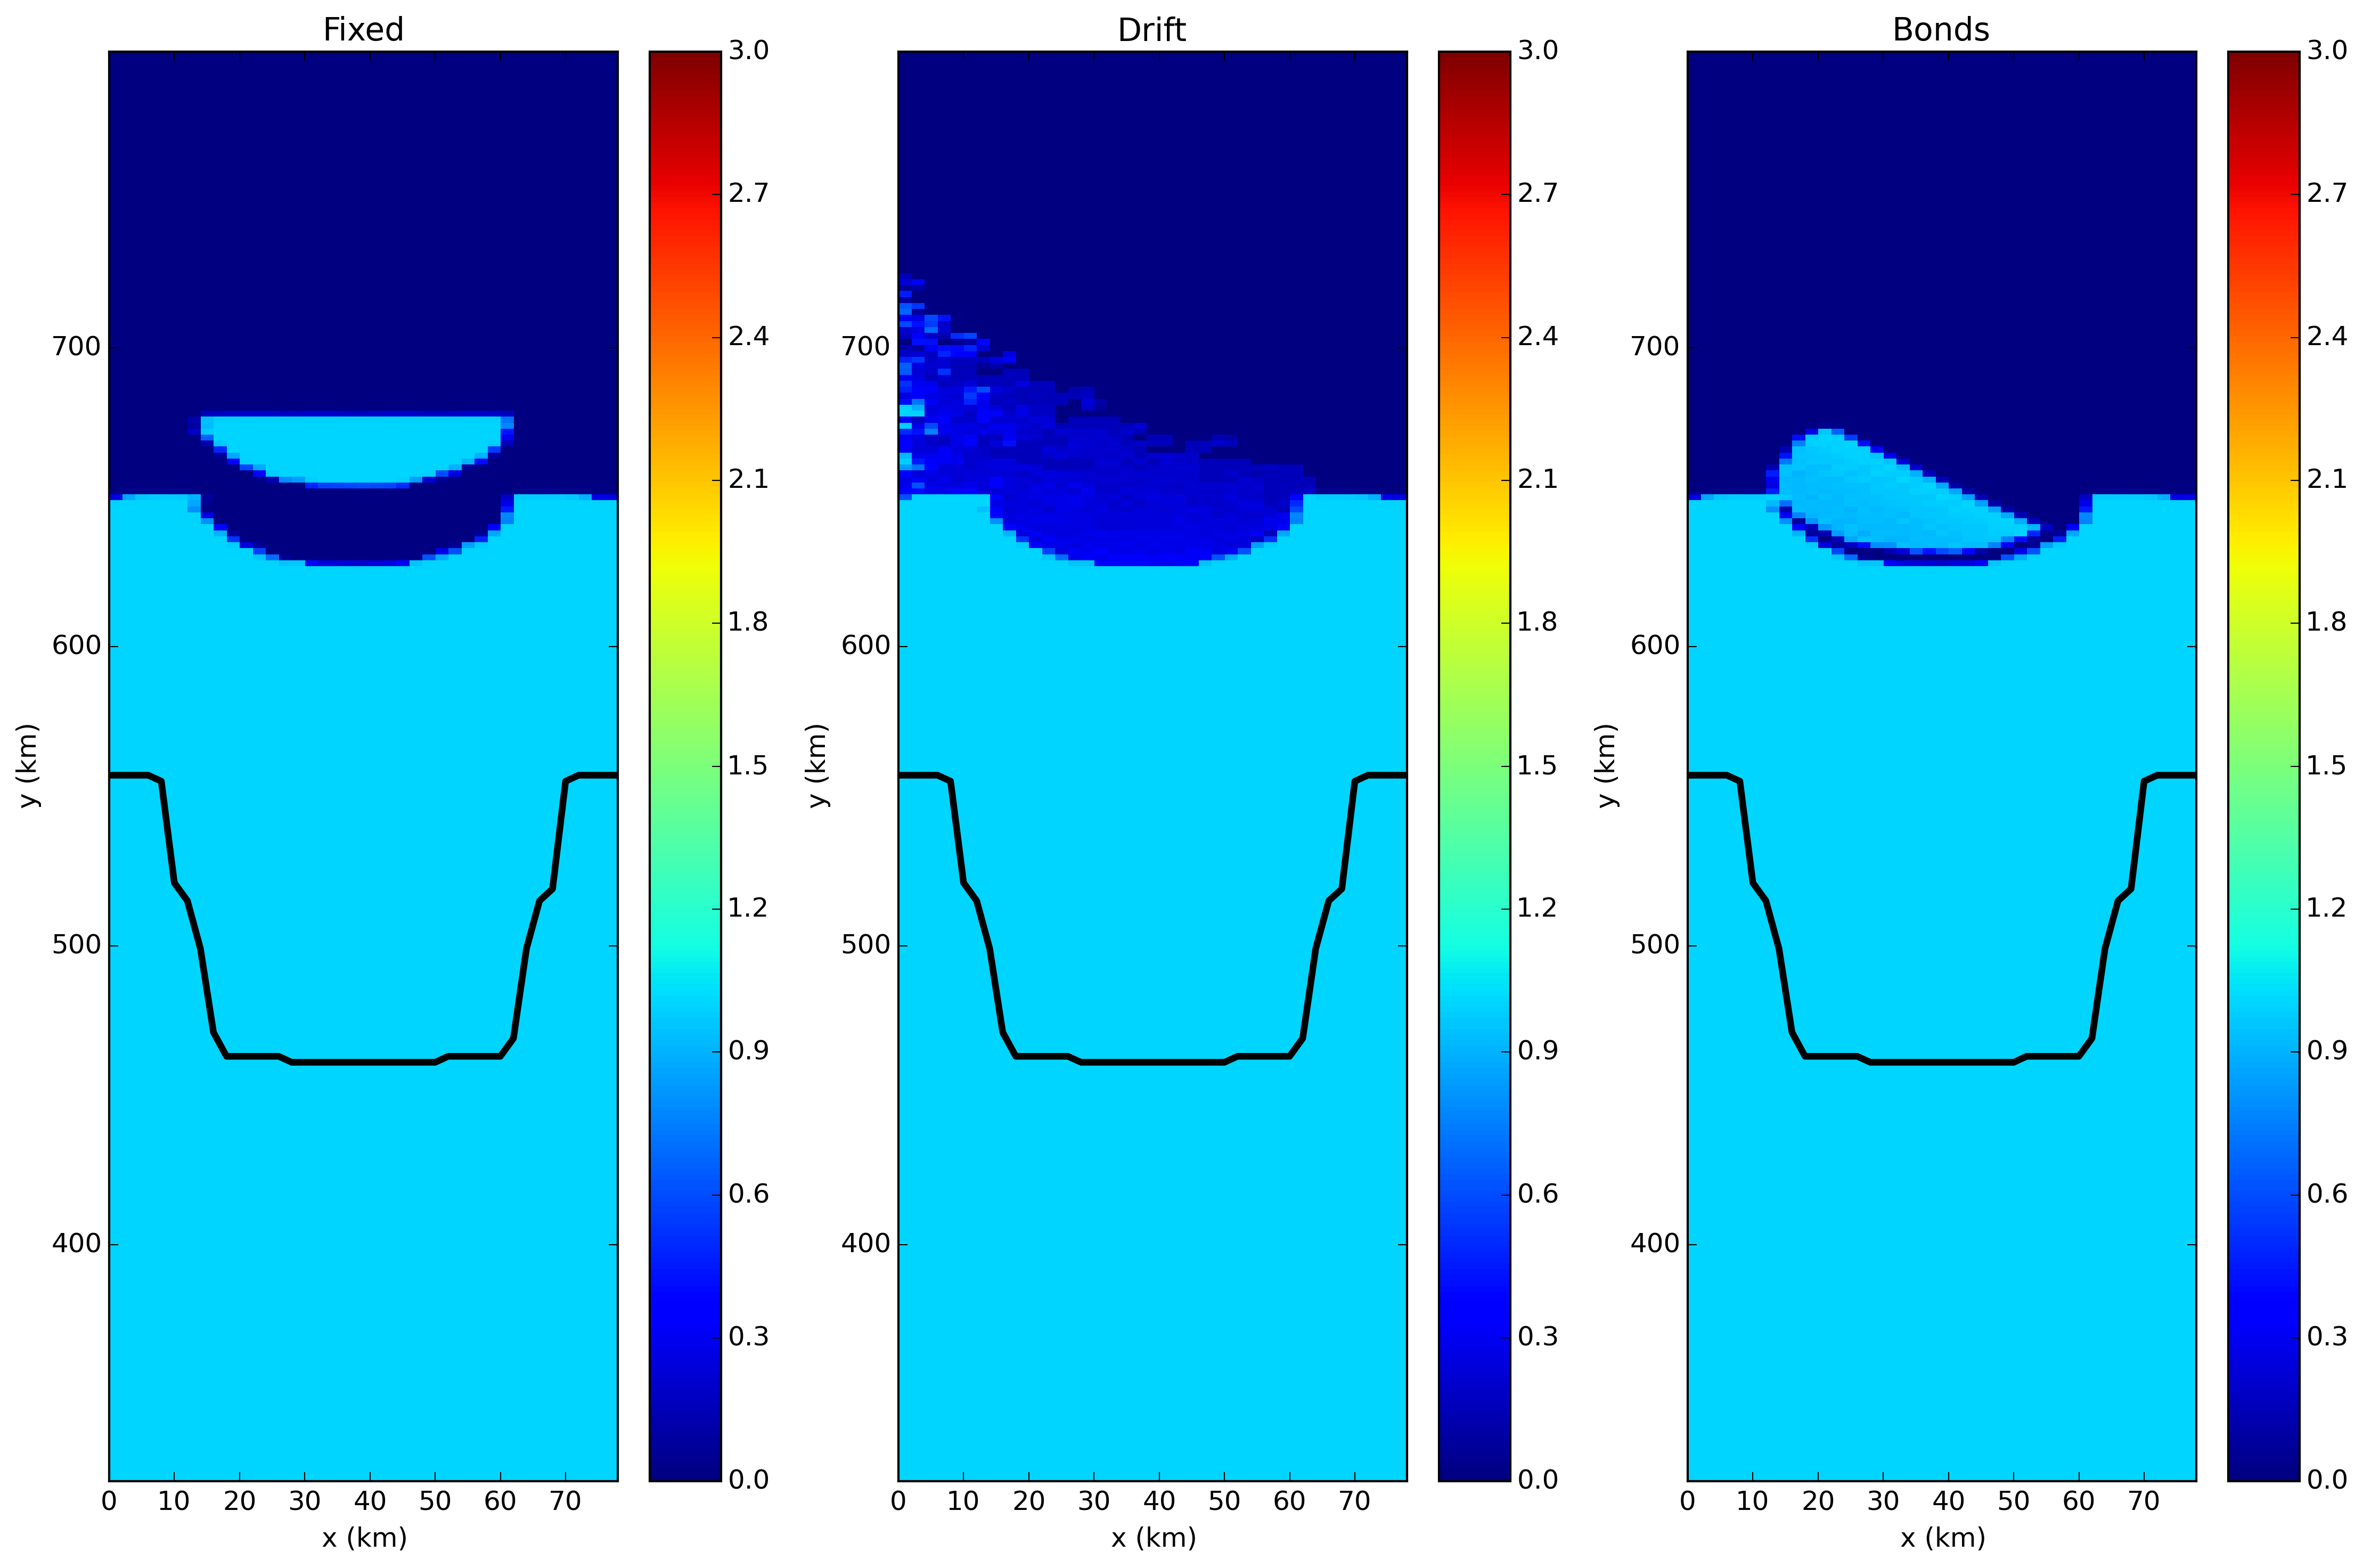
\includegraphics[width=0.99\textwidth]{/Users/alon/Desktop/files/Icebergs_clusters/Towards_Publication/Tech_paper/Github_stuff/Tech-paper/Figures/fixed_drift_bond_spread_area.png}
%\caption{ {Need to update this Figure. Also, I should try using orientation with the Bonds.}}
%\end{center}
%FIgure created by \end{center}
%\label{fig:}
%\end{figure}


% \clearpage

%\begin{figure}
%\begin{center}
%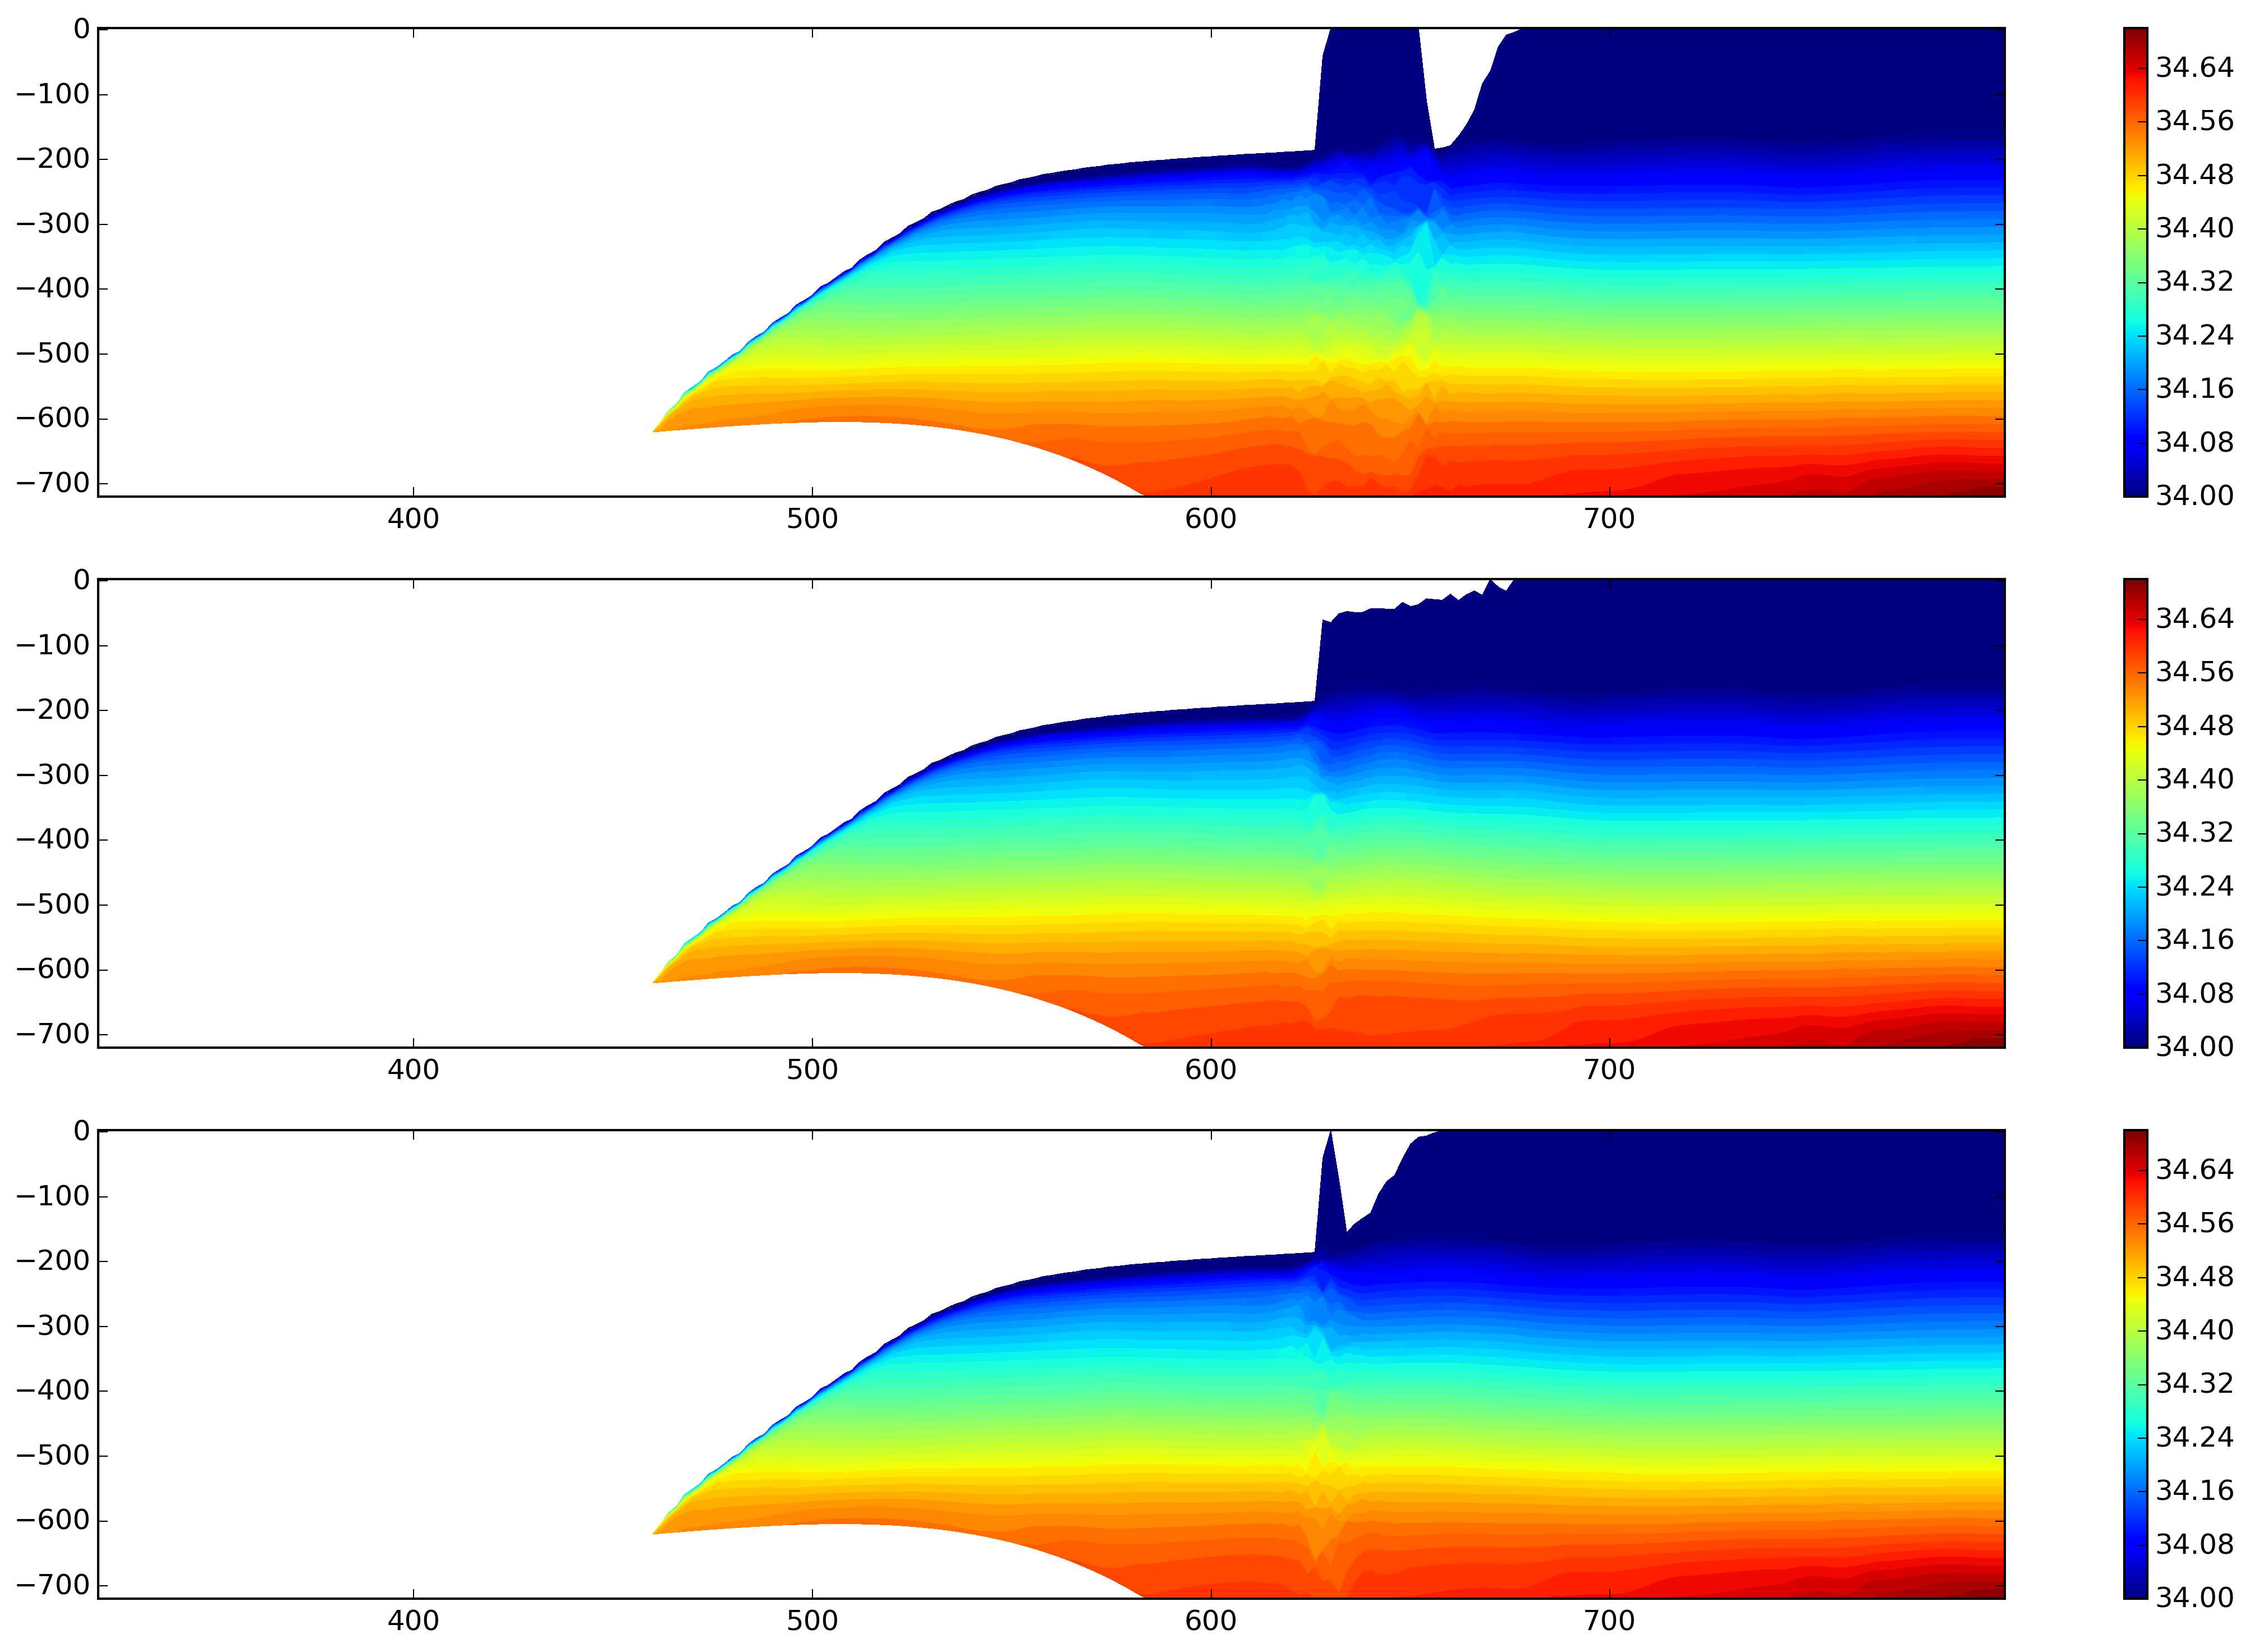
\includegraphics[width=0.99\textwidth]{/Users/alon/Desktop/files/Icebergs_clusters/Towards_Publication/Tech_paper/Github_stuff/Tech-paper/Figures/fixed_drift_bond_salt_layers.png}
%\caption{ {}}
%\end{center}
%FIgure created by \end{center}
%\label{fig:}
%\end{figure}

%\clearpage

%\begin{figure}
%\begin{center}
%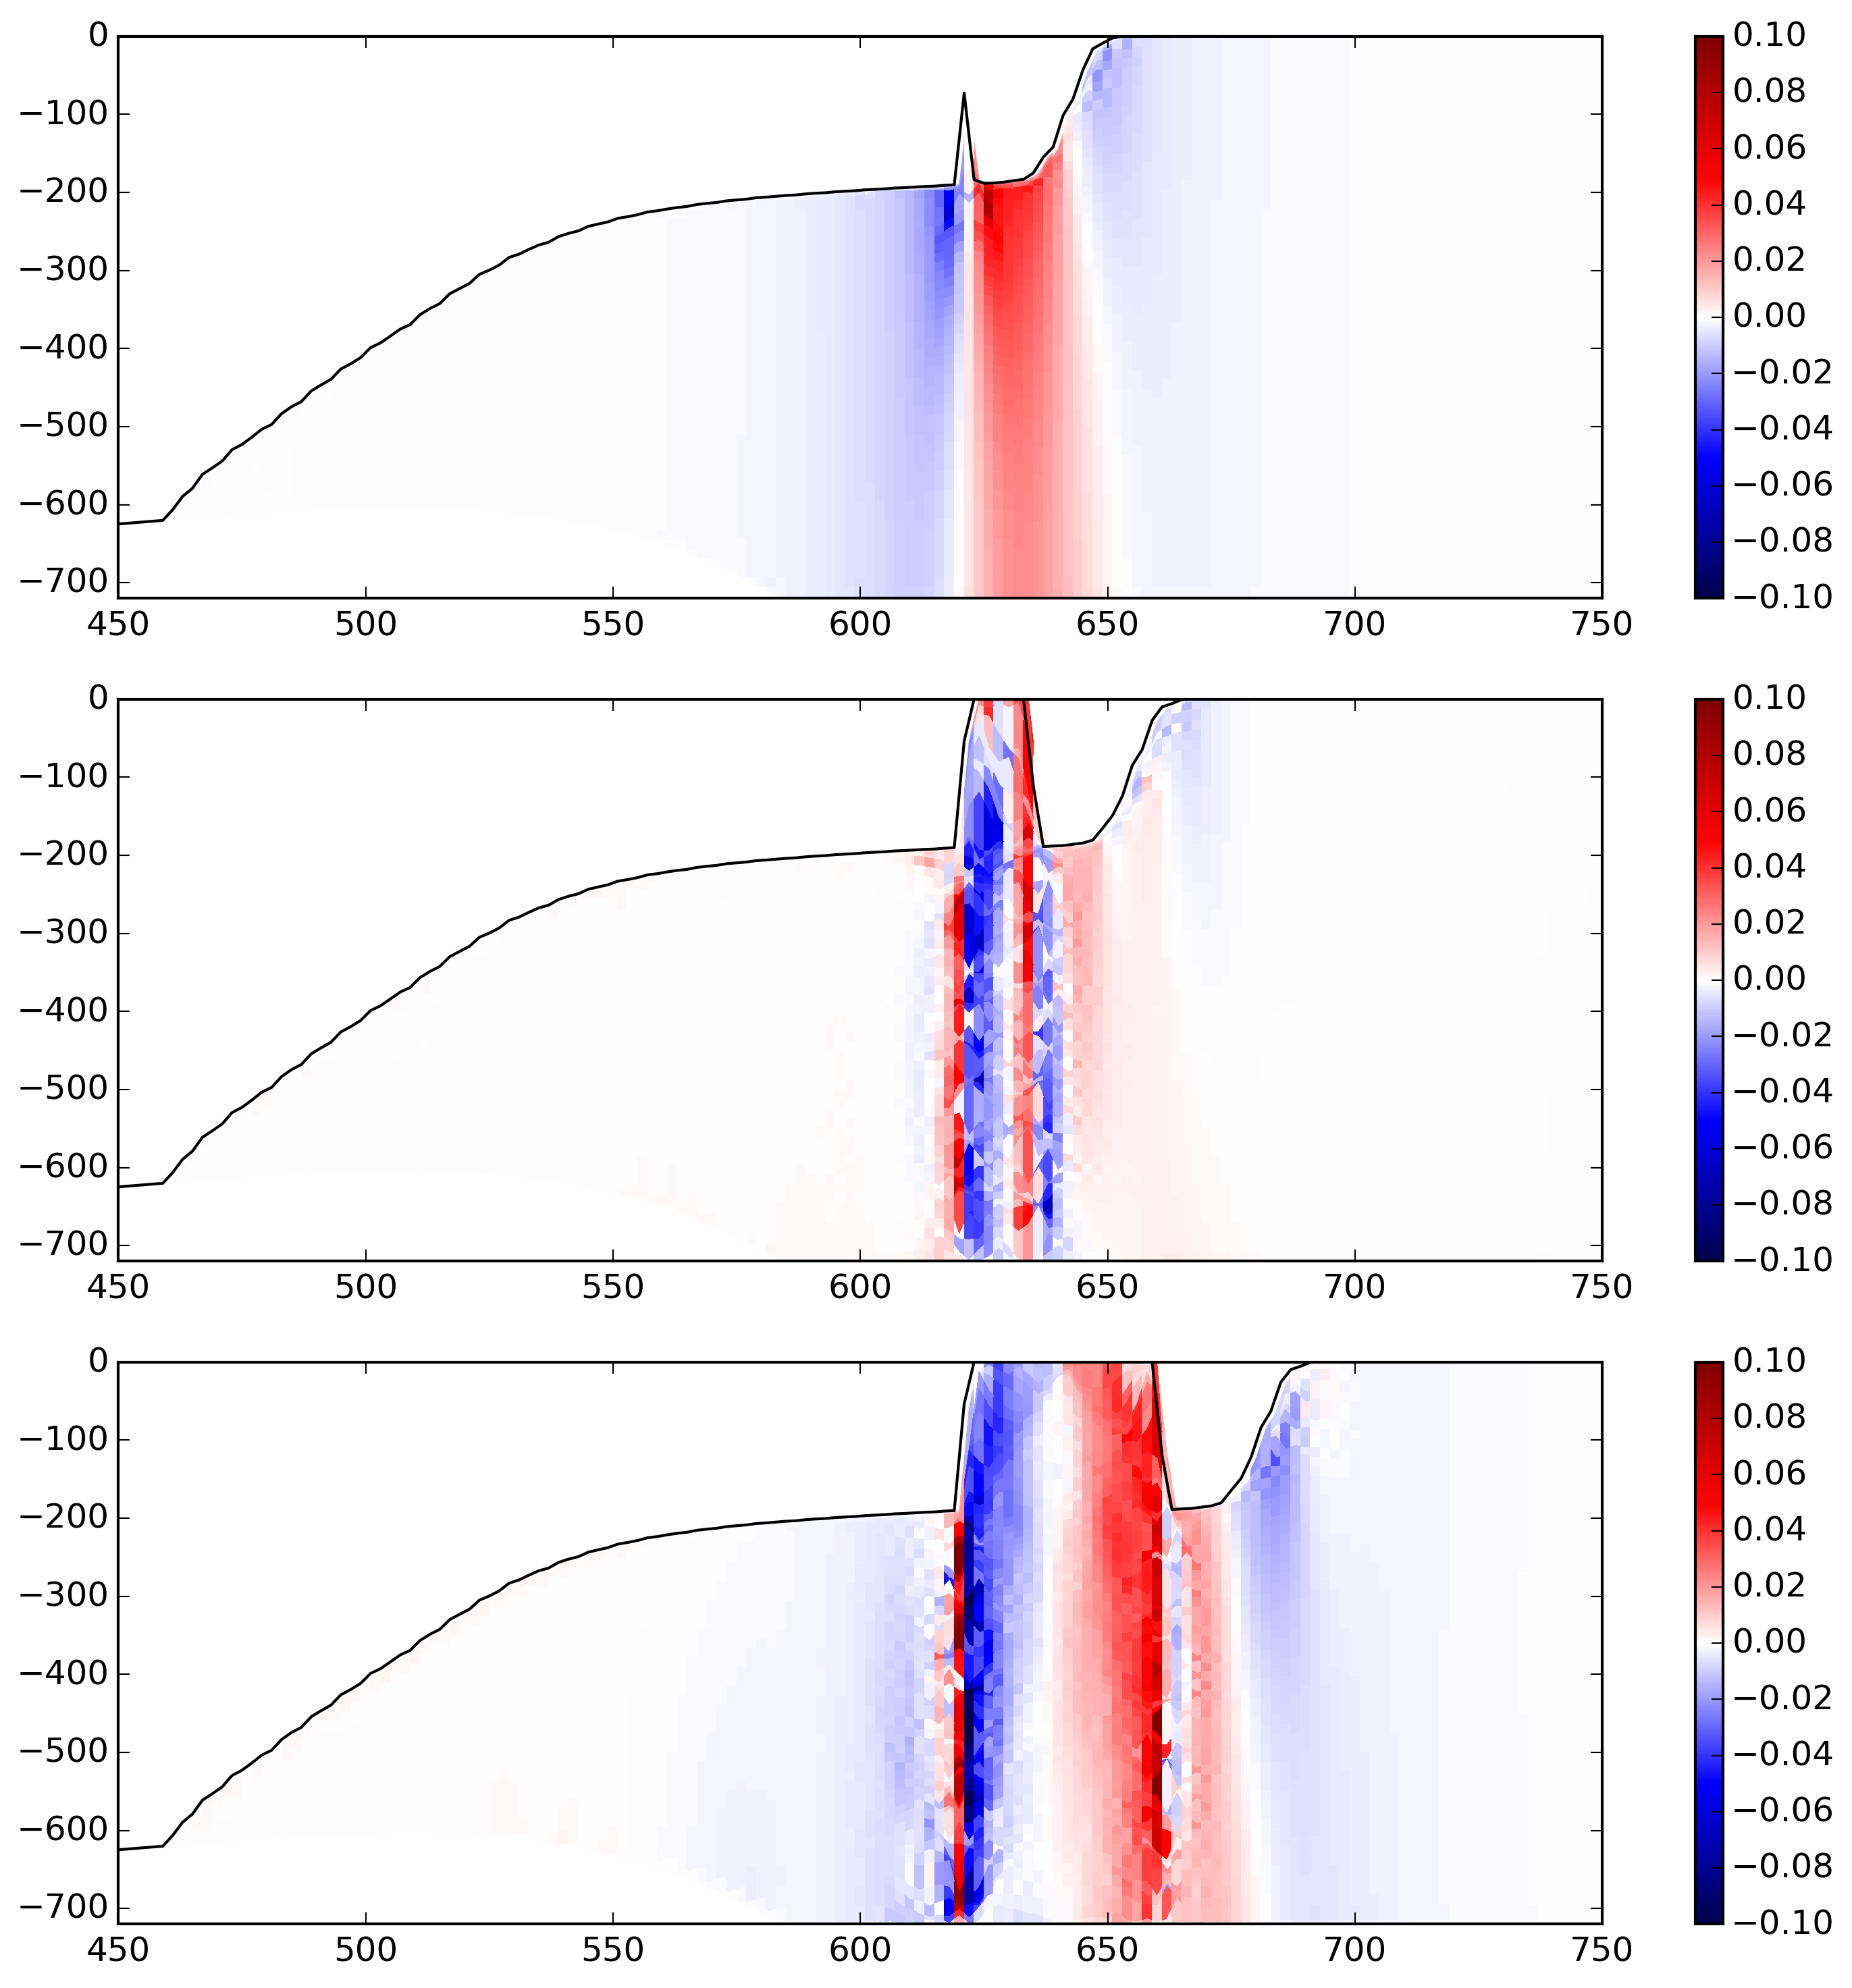
\includegraphics[width=0.99\textwidth]{/Users/alon/Desktop/files/Icebergs_clusters/Towards_Publication/Tech_paper/Github_stuff/Tech-paper/Figures/snapshots_fixed_01_u_layers.png}
%\caption{ {Need to update this Figure. }}
%\end{center}
%FIgure created by \end{center}
%\label{fig:}
%\end{figure}


%\clearpage

%\begin{figure}
%\begin{center}
%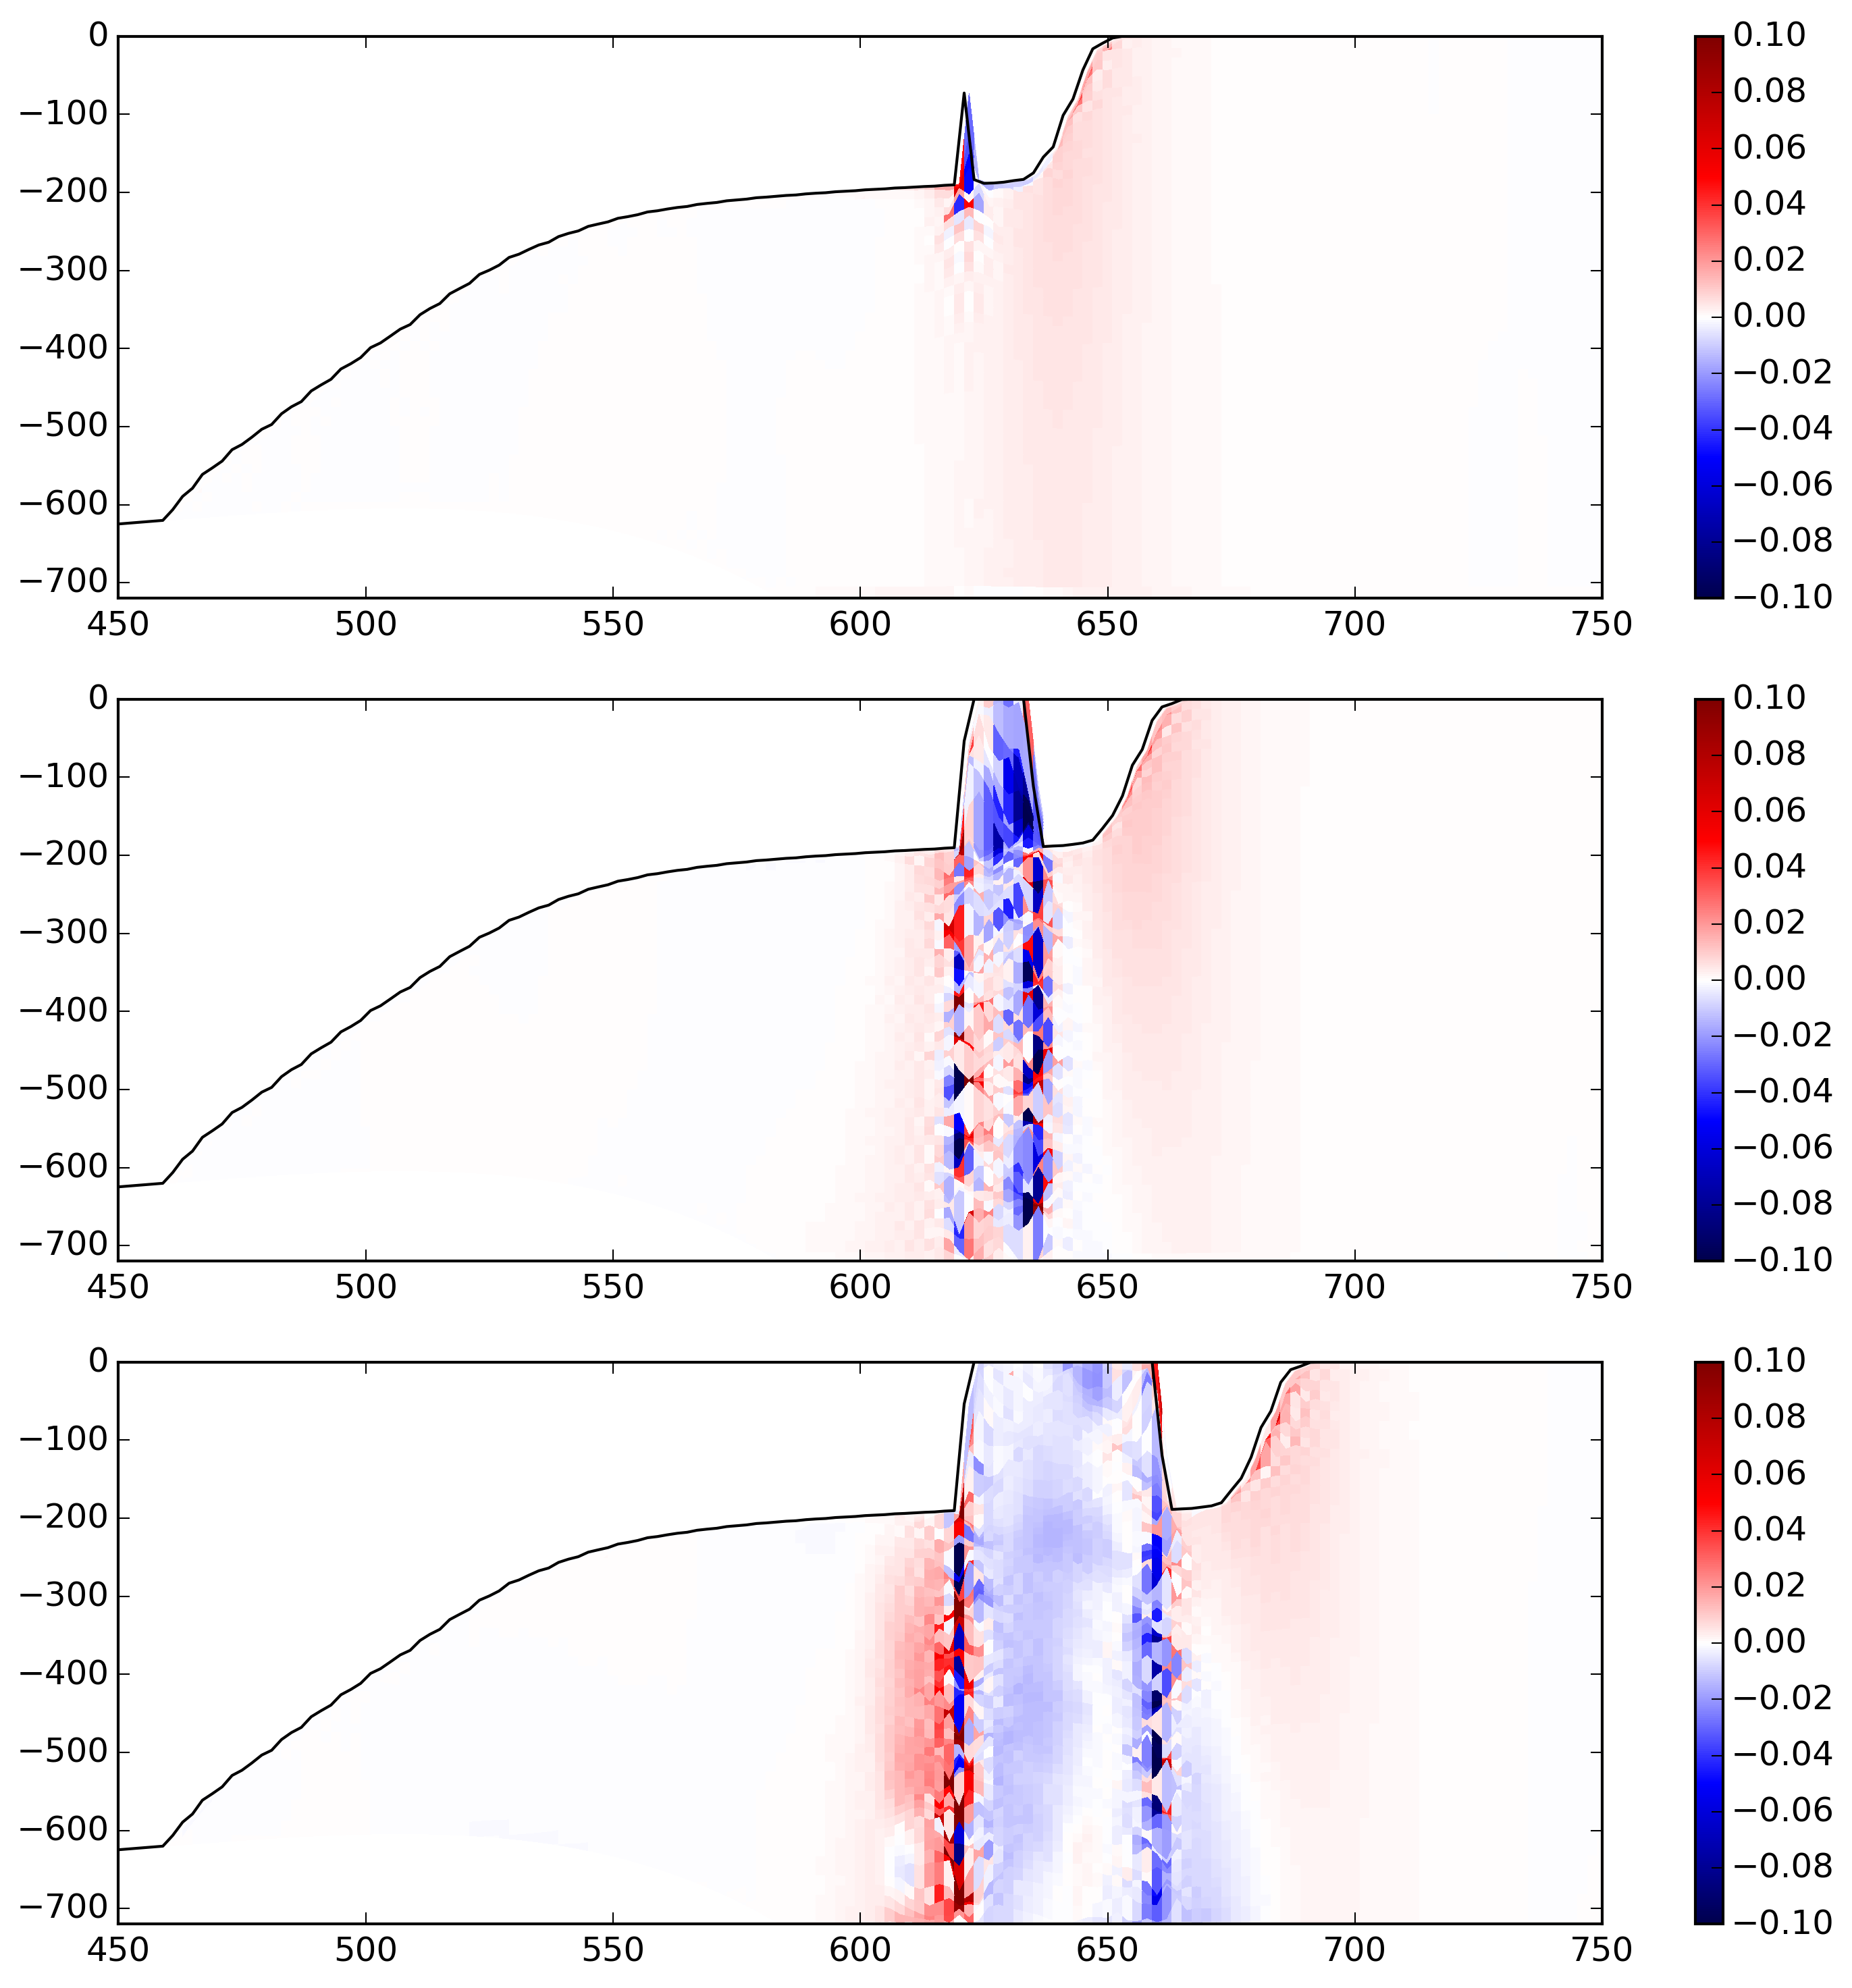
\includegraphics[width=0.99\textwidth]{/Users/alon/Desktop/files/Icebergs_clusters/Towards_Publication/Tech_paper/Github_stuff/Tech-paper/Figures/snapshots_fixed_01_v_layers.png}
%\caption{ {Need to update this Figure. }}
%\end{center}
%FIgure created by \end{center}
%\label{fig:}
%\end{figure}
\clearpage
\section{Supplementary Figures}
\clearpage

\setcounter{figure}{0}
\renewcommand{\thefigure}{S\arabic{figure}}





\begin{figure}
\begin{center}
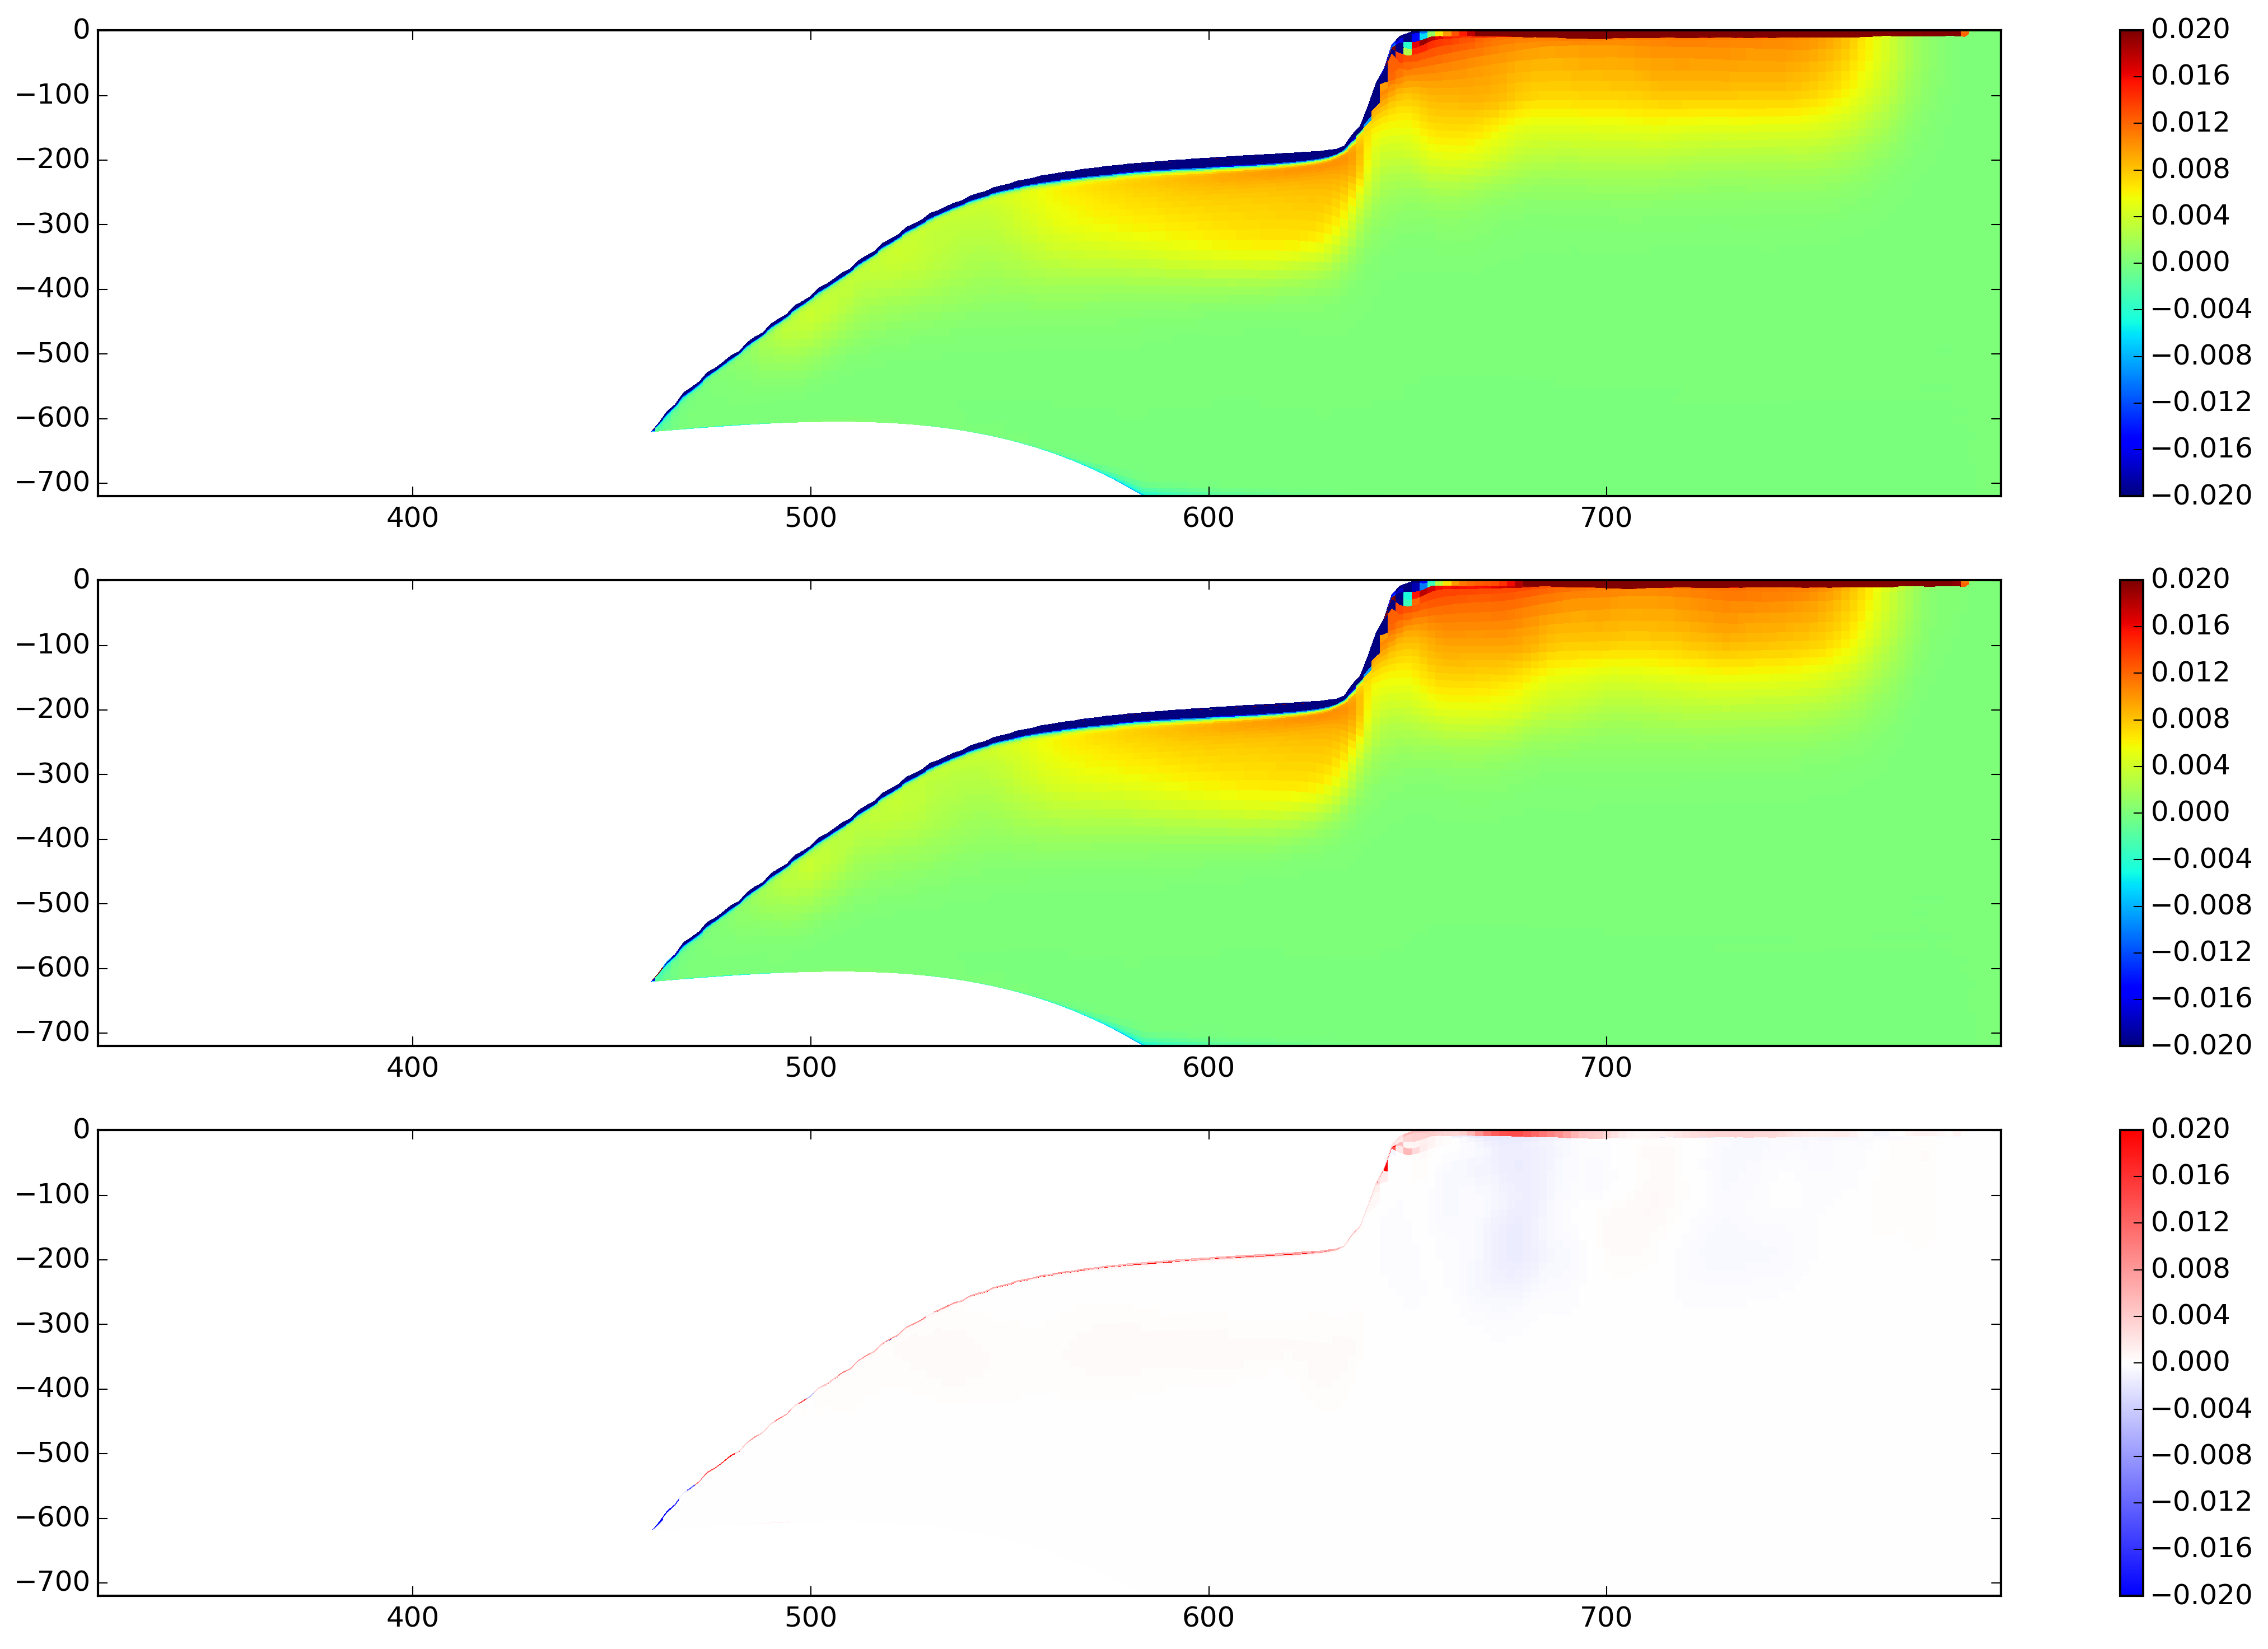
\includegraphics[width=0.99\textwidth]{/Users/alon/Desktop/files/Icebergs_clusters/Towards_Publication/Tech_paper/Github_stuff/Tech-paper/Figures/static_shelf_comparison_salt_layers.png}
\caption{ {Comparison of Eulerian ice shelf model and Lagrangian Ice shelf model salinity fields.}}
\end{center}
%FIgure created by \end{center}
\label{fig:Salt_comparison}
\end{figure}
 \clearpage

 
 
\begin{figure}
\begin{center}
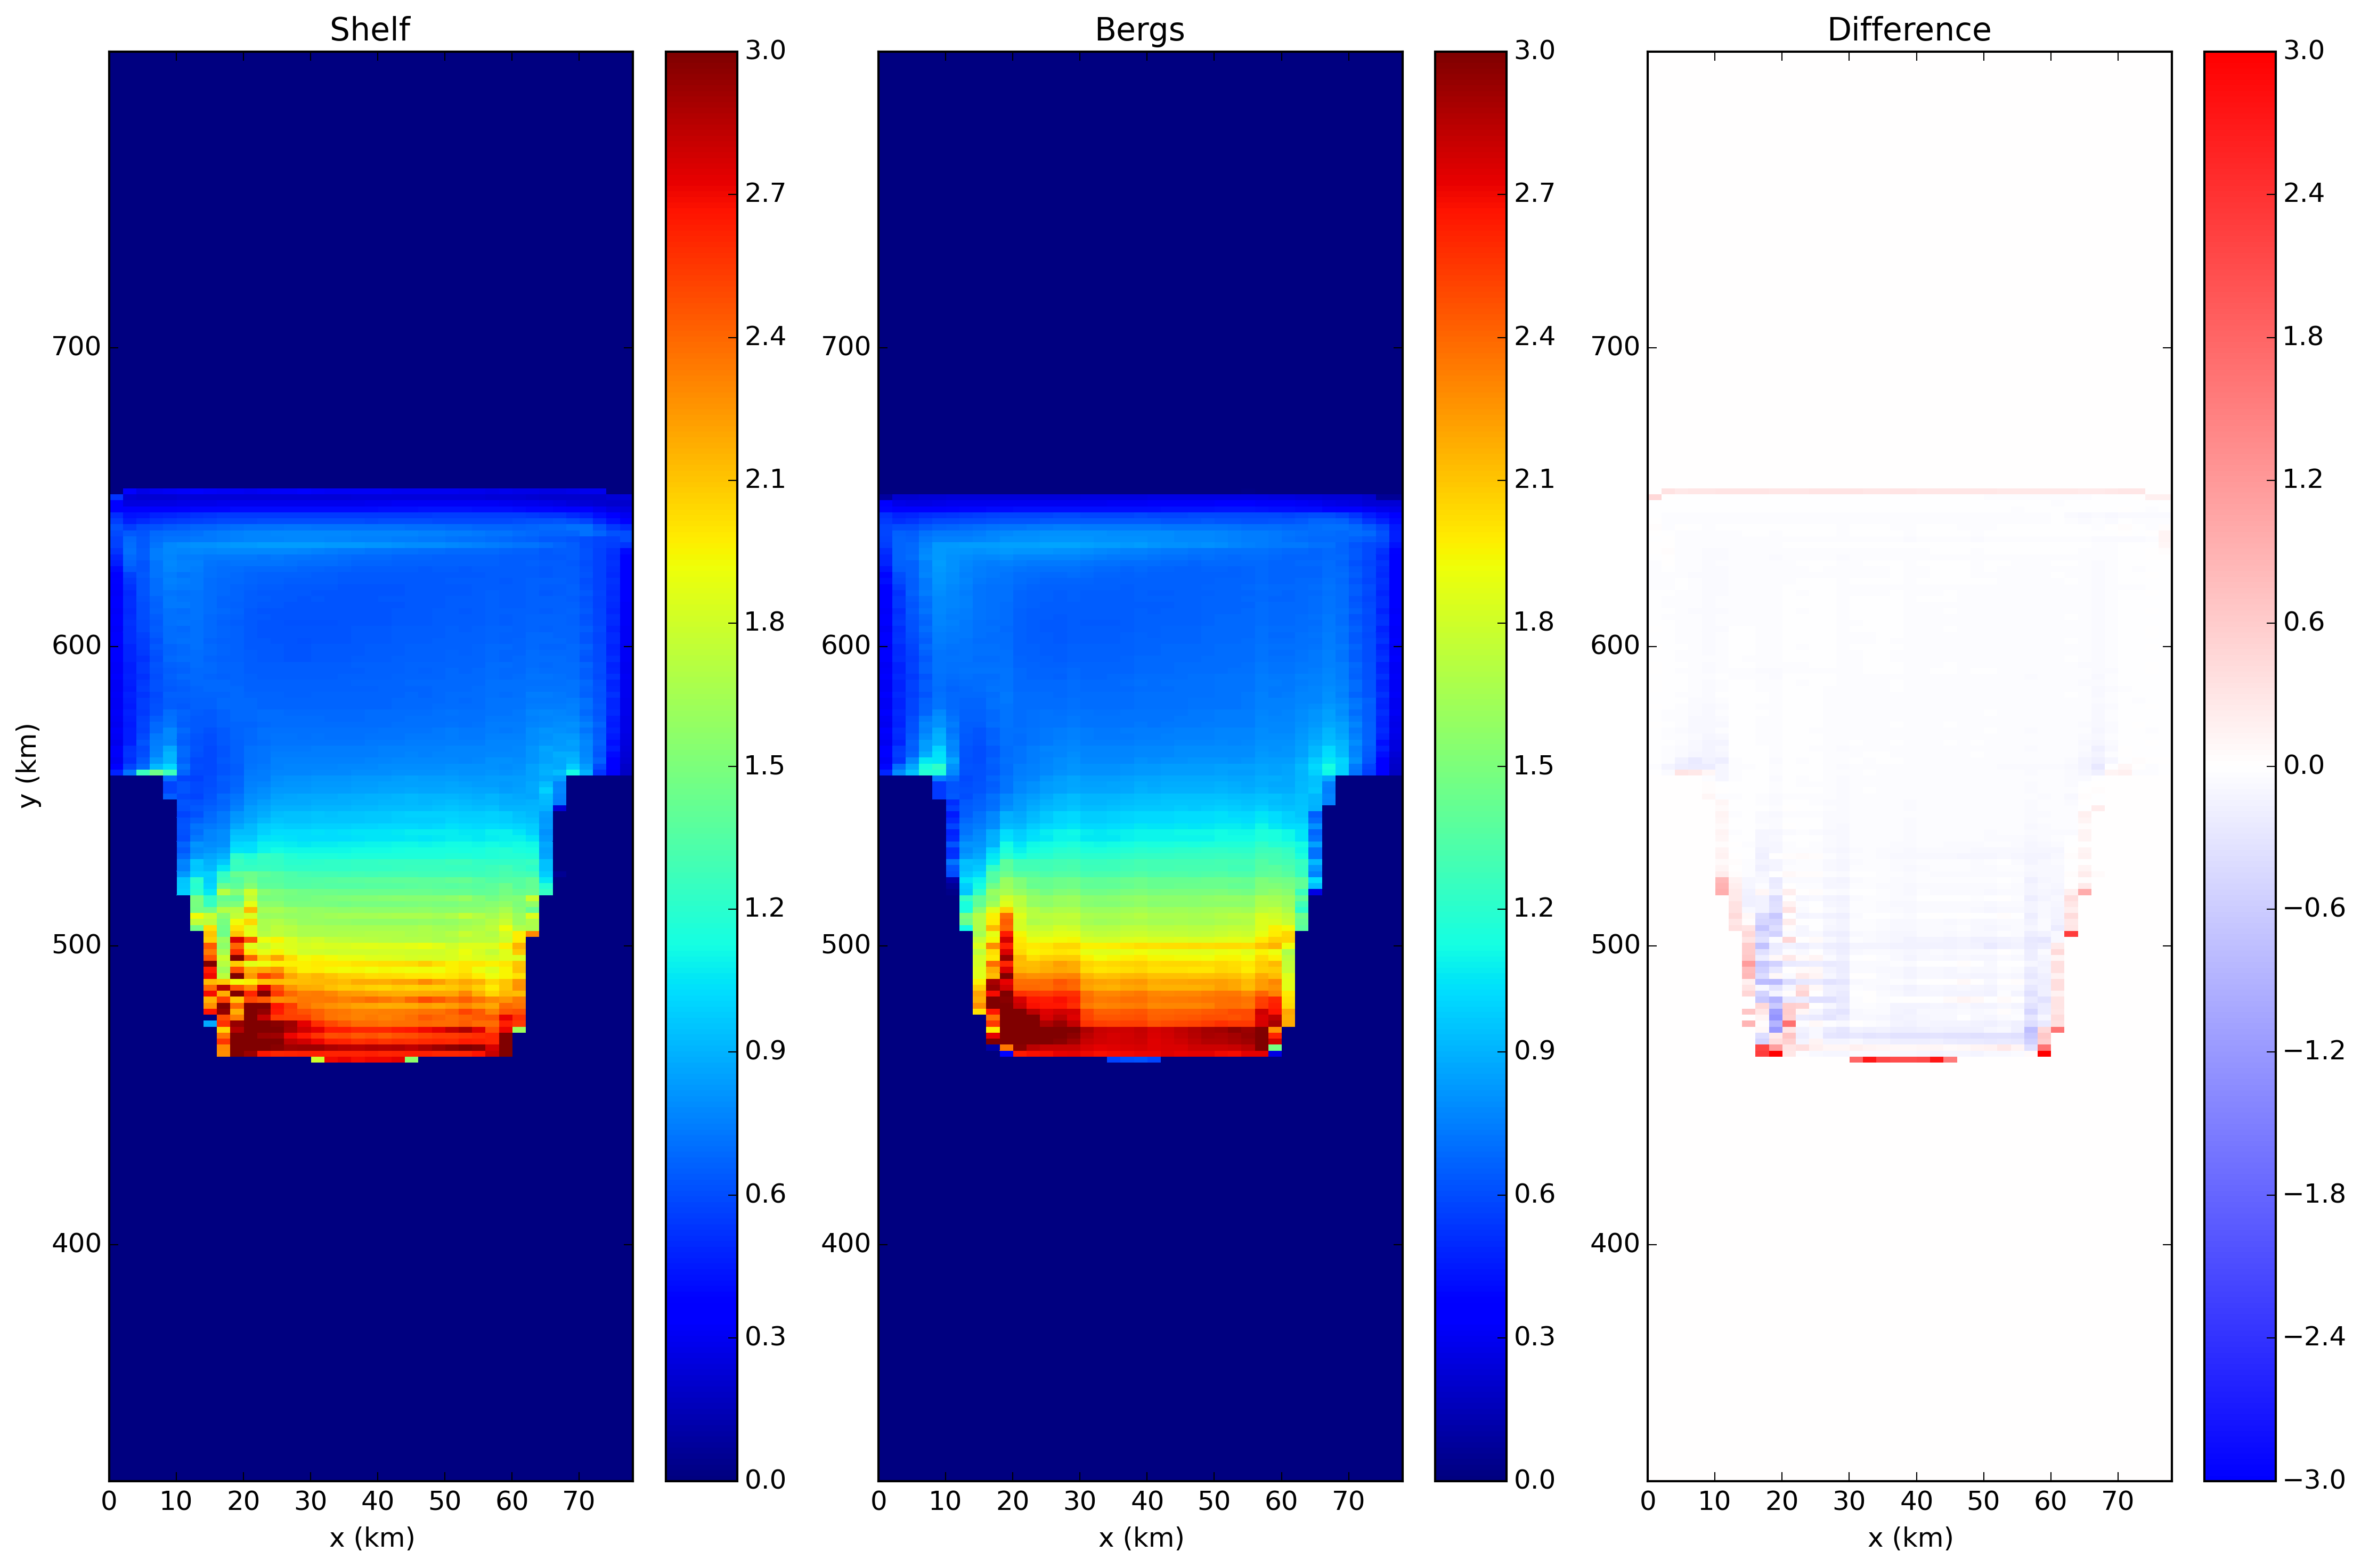
\includegraphics[width=0.99\textwidth]{/Users/alon/Desktop/files/Icebergs_clusters/Towards_Publication/Tech_paper/Github_stuff/Tech-paper/Figures/static_shelf_comparison_melt.png}
\caption{ {Comparison of Eulerian ice shelf model and Lagrangian Ice shelf model melt fields.}}
\end{center}
%FIgure created by \end{center}
\label{fig:Melt_comparison}
\end{figure}
 \clearpage


\begin{figure}
\begin{center}
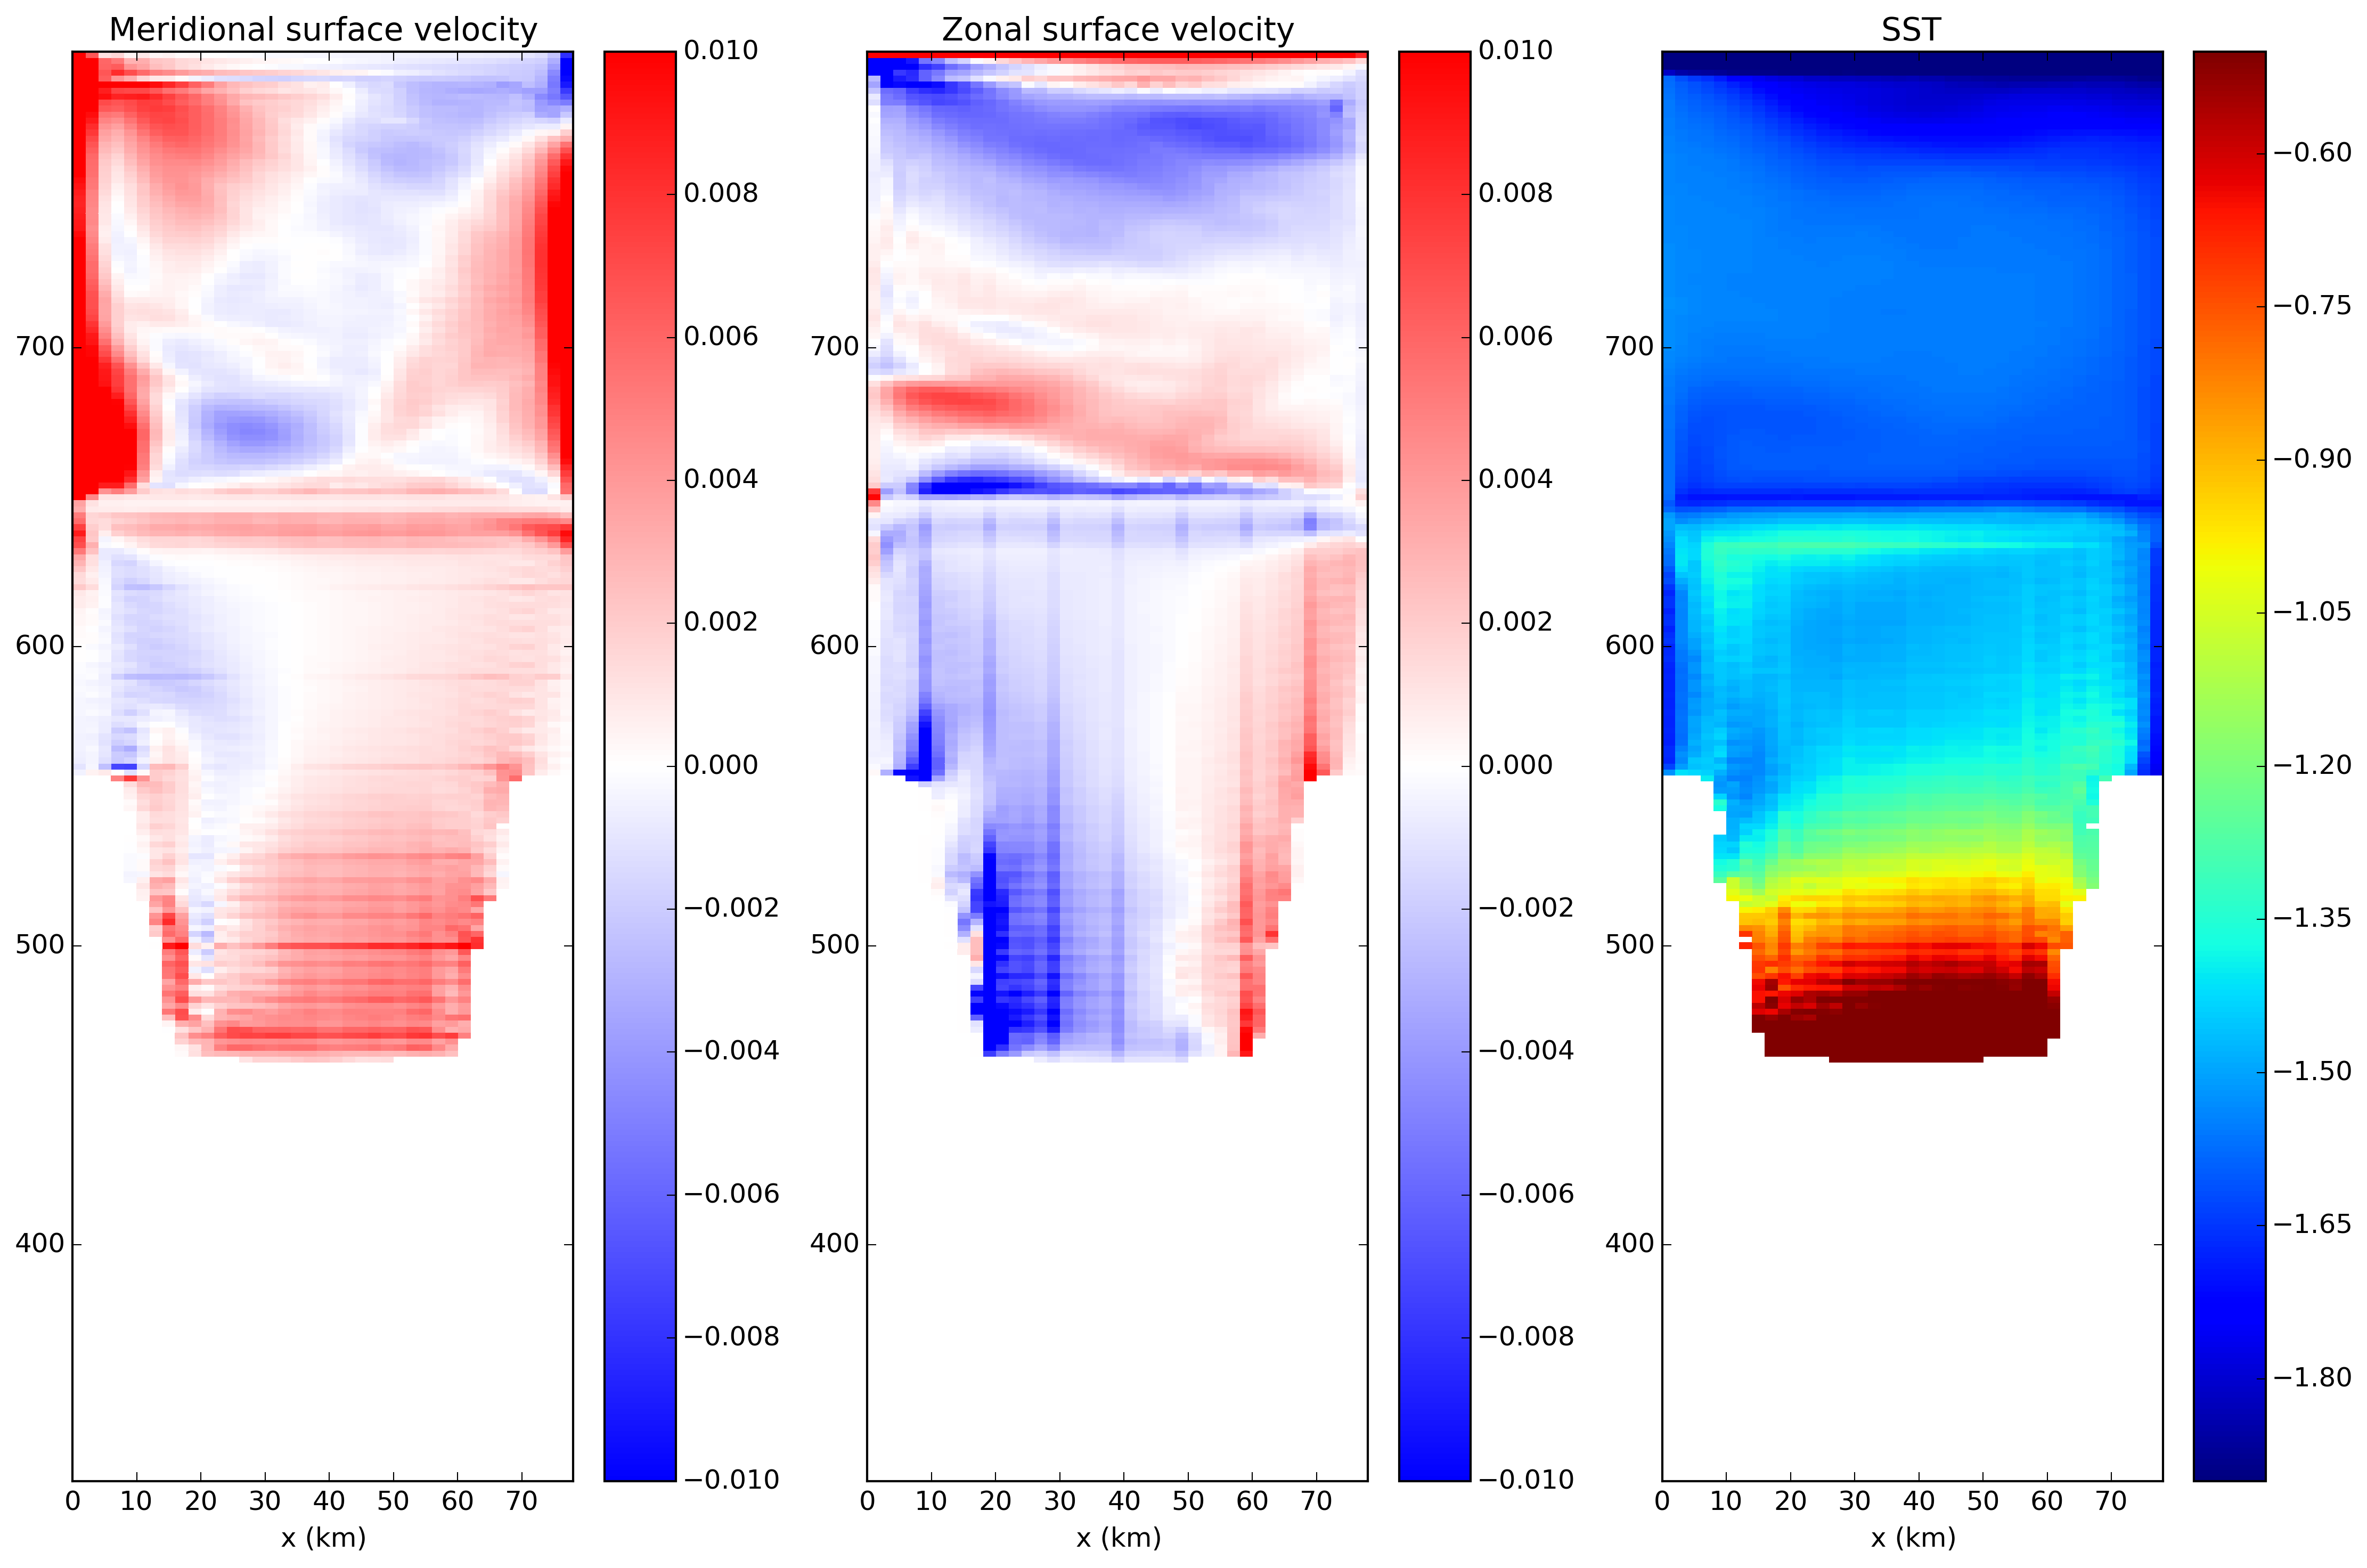
\includegraphics[width=0.99\textwidth]{/Users/alon/Desktop/files/Icebergs_clusters/Towards_Publication/Tech_paper/Github_stuff/Tech-paper/Figures/static_shelf_solo_vo_uo_sst.png}
\caption{ {Results of the static ice shelf experiment using the LIISM model. The three panels show 5 year time average of the (a) meridional velocity, (b) zonal velocity and (c) ocean temperature in the top layer of the simulation (at the surface or directly below the ice shelf).}}
\end{center}
%FIgure created by \end{center}
\label{fig:static_solo}
\end{figure} 
 \clearpage
 

 \end{document}

%%%%%%%%%%%%%%%%%%%%%%%%%%%%%%%%%%%%%%%%%%%%%%%%%%%%%%%%%%%%%%%

